\documentclass[14pt,a4paper]{extarticle}
\usepackage[utf8]{inputenc}
\usepackage[ukrainian]{babel}
\usepackage{geometry}
\geometry{left=3cm,right=1cm,top=2cm,bottom=2cm}
\usepackage{indentfirst}
\usepackage{setspace}
\onehalfspacing
\usepackage{tikz}
\usepackage{pgf-umlcd}
\usepackage{pgf-umlsd}
\usetikzlibrary{shapes,arrows,positioning,calc,fit}
\usepackage{graphicx}
\usepackage{listings}
\usepackage{xcolor}
\usepackage{hyperref}
\usepackage{tocloft}
\usepackage{titlesec}

% Налаштування відступів для розділів
\titleformat{\section}
  {\normalfont\fontsize{14}{16}\bfseries}{\thesection}{1em}{}
\titleformat{\subsection}
  {\normalfont\fontsize{14}{16}\bfseries}{\thesubsection}{1em}{}

% Налаштування змісту
\renewcommand{\cftsecleader}{\cftdotfill{\cftdotsep}}

\begin{document}

% Титульна сторінка
\begin{titlepage}
\centering
\textbf{МІНІСТЕРСТВО ОСВІТИ І НАУКИ УКРАЇНИ}\\
\textbf{[НАЗВА УНІВЕРСИТЕТУ]}\\[0.5cm]
\textbf{Факультет [назва факультету]}\\
\textbf{Кафедра [назва кафедри]}\\[3cm]

{\Large\textbf{КУРСОВА РОБОТА}}\\[0.5cm]
з дисципліни «[Назва дисципліни]»\\[0.5cm]
на тему:\\[0.5cm]
{\Large\textbf{«ІНФОРМАЦІЙНА СИСТЕМА УПРАВЛІННЯ\\АТЕЛЬЄ»}}\\[3cm]

\begin{flushright}
Виконав:\\
студент групи [номер групи]\\
[ПІБ студента]\\[1cm]
Перевірив:\\
[ПІБ викладача]\\
[посада, науковий ступінь]
\end{flushright}

\vfill

Місто, 2025
\end{titlepage}

\newpage
\tableofcontents
\newpage

\section{ВСТУП}

\subsection{Актуальність теми}

Сучасний розвиток інформаційних технологій створює нові можливості для автоматизації бізнес-процесів у різних галузях економіки. Ательє як підприємство, що надає послуги з пошиття та ремонту одягу, потребує ефективної системи управління для підвищення якості обслуговування клієнтів та оптимізації виробничих процесів.

Актуальність розробки інформаційної системи для ательє обумовлена наступними факторами:
\begin{itemize}
    \item необхідність автоматизації обліку замовлень та клієнтів;
    \item потреба у контролі виконання замовлень та завантаженості працівників;
    \item важливість ведення складського обліку матеріалів;
    \item необхідність формування звітності для аналізу діяльності підприємства;
    \item підвищення конкурентоспроможності за рахунок покращення якості обслуговування.
\end{itemize}

\subsection{Мета та завдання курсової роботи}

\textbf{Мета роботи:} розробка інформаційної системи управління ательє для автоматизації основних бізнес-процесів підприємства.

\textbf{Завдання роботи:}
\begin{enumerate}
    \item Проаналізувати предметну область та виявити основні бізнес-процеси ательє;
    \item Визначити функціональні вимоги до інформаційної системи;
    \item Розробити діаграми прецедентів для визначення взаємодії користувачів з системою;
    \item Створити діаграму класів для опису структури системи;
    \item Розробити модель бази даних;
    \item Описати архітектуру системи;
    \item Розробити діаграми діяльності для ключових бізнес-процесів.
\end{enumerate}

\subsection{Об'єкт та предмет дослідження}

\textbf{Об'єкт дослідження:} бізнес-процеси ательє з пошиття та ремонту одягу.

\textbf{Предмет дослідження:} методи та засоби автоматизації управління діяльністю ательє.

\newpage
\section{АНАЛІЗ ПРЕДМЕТНОЇ ОБЛАСТІ}

\subsection{Опис предметної області}

Ательє --- це підприємство, що надає послуги з пошиття одягу на замовлення, ремонту та підгонки одягу за розміром клієнта. Основними процесами ательє є:

\begin{itemize}
    \item \textbf{Прийом замовлень} --- консультація клієнта, зняття мірок, вибір тканини та фасону, визначення вартості та термінів виконання;
    \item \textbf{Виробництво} --- розкрій тканини, пошиття виробу, примірка та коригування;
    \item \textbf{Видача замовлень} --- перевірка якості, розрахунок з клієнтом, видача готового виробу;
    \item \textbf{Складський облік} --- облік тканин, фурнітури та інших матеріалів;
    \item \textbf{Управління персоналом} --- розподіл замовлень між кравцями, облік робочого часу.
\end{itemize}

\subsection{Основні сутності предметної області}

\begin{enumerate}
    \item \textbf{Клієнт} --- особа, яка замовляє послуги ательє;
    \item \textbf{Замовлення} --- конкретне замовлення клієнта на виготовлення або ремонт виробу;
    \item \textbf{Працівник} --- співробітник ательє (кравець, закрійник, адміністратор);
    \item \textbf{Послуга} --- вид роботи (пошиття сукні, ремонт брюк, підгонка піджака тощо);
    \item \textbf{Матеріал} --- тканина, фурнітура та інші матеріали;
    \item \textbf{Мірки} --- індивідуальні параметри клієнта.
\end{enumerate}

\subsection{Функціональні вимоги до системи}

Інформаційна система управління ательє повинна забезпечувати:

\begin{enumerate}
    \item \textbf{Управління клієнтами:}
    \begin{itemize}
        \item реєстрація нових клієнтів;
        \item зберігання контактної інформації;
        \item зберігання мірок клієнтів;
        \item історія замовлень клієнта.
    \end{itemize}
    
    \item \textbf{Управління замовленнями:}
    \begin{itemize}
        \item створення нових замовлень;
        \item відстеження статусу виконання;
        \item призначення виконавців;
        \item розрахунок вартості;
        \item контроль термінів виконання.
    \end{itemize}
    
    \item \textbf{Управління матеріалами:}
    \begin{itemize}
        \item облік наявності матеріалів на складі;
        \item облік витрачання матеріалів на замовлення;
        \item контроль залишків та формування замовлень постачальникам.
    \end{itemize}
    
    \item \textbf{Управління персоналом:}
    \begin{itemize}
        \item облік працівників;
        \item розподіл замовлень між виконавцями;
        \item контроль завантаженості.
    \end{itemize}
    
    \item \textbf{Звітність:}
    \begin{itemize}
        \item звіт по виконаних замовленнях;
        \item фінансовий звіт;
        \item звіт по завантаженості працівників;
        \item звіт по залишках матеріалів.
    \end{itemize}
\end{enumerate}

\newpage
\section{ПРОЕКТУВАННЯ ІНФОРМАЦІЙНОЇ СИСТЕМИ}

\subsection{Діаграма прецедентів}

Діаграма прецедентів (use case diagram) відображає взаємодію користувачів з системою та основні функції, які вона надає.

\begin{figure}[h!]
\centering
\begin{tikzpicture}[scale=0.9, every node/.style={scale=0.85}]
    % Стиль для акторів
    \tikzstyle{actor}=[stick figure, minimum size=1.2cm, thick]
    
    % Актори зліва
    \node at (-4,6) {\textbf{Клієнт}};
    \draw[thick] (-4,5.5) circle (0.3cm);
    \draw[thick] (-4,5.2) -- (-4,4.2);
    \draw[thick] (-4.5,4.7) -- (-4,5) -- (-3.5,4.7);
    \draw[thick] (-4.5,3.7) -- (-4,4.2) -- (-3.5,3.7);
    
    \node at (-4,2) {\textbf{Адміністратор}};
    \draw[thick] (-4,1.5) circle (0.3cm);
    \draw[thick] (-4,1.2) -- (-4,0.2);
    \draw[thick] (-4.5,0.7) -- (-4,1) -- (-3.5,0.7);
    \draw[thick] (-4.5,-0.3) -- (-4,0.2) -- (-3.5,-0.3);
    
    \node at (-4,-3) {\textbf{Кравець}};
    \draw[thick] (-4,-3.5) circle (0.3cm);
    \draw[thick] (-4,-3.8) -- (-4,-4.8);
    \draw[thick] (-4.5,-4.3) -- (-4,-4) -- (-3.5,-4.3);
    \draw[thick] (-4.5,-5.3) -- (-4,-4.8) -- (-3.5,-5.3);
    
    % Межа системи
    \draw[thick] (-0.5,-6.5) rectangle (11,7);
    \node at (5.2,6.6) {\textbf{Система управління ательє}};
    
    % Прецеденти для клієнта
    \node[ellipse, draw, thick, text width=2.2cm, align=center, minimum height=1.2cm] (uc1) at (2,5.5) {\small Переглянути\\каталог послуг};
    \node[ellipse, draw, thick, text width=2.2cm, align=center, minimum height=1.2cm] (uc2) at (6,5.5) {\small Оформити\\замовлення};
    \node[ellipse, draw, thick, text width=2.2cm, align=center, minimum height=1.2cm] (uc3) at (9,5.5) {\small Переглянути\\статус};
    
    % Прецеденти для адміністратора
    \node[ellipse, draw, thick, text width=2.2cm, align=center, minimum height=1.2cm] (uc4) at (1,2.5) {\small Керування\\клієнтами};
    \node[ellipse, draw, thick, text width=2.2cm, align=center, minimum height=1.2cm] (uc5) at (4,2.5) {\small Керування\\замовленнями};
    \node[ellipse, draw, thick, text width=2.2cm, align=center, minimum height=1.2cm] (uc6) at (7,2.5) {\small Керування\\послугами};
    \node[ellipse, draw, thick, text width=2.2cm, align=center, minimum height=1.2cm] (uc7) at (1,-0.5) {\small Керування\\матеріалами};
    \node[ellipse, draw, thick, text width=2.2cm, align=center, minimum height=1.2cm] (uc8) at (4,-0.5) {\small Керування\\персоналом};
    \node[ellipse, draw, thick, text width=2.2cm, align=center, minimum height=1.2cm] (uc9) at (7,-0.5) {\small Формування\\звітів};
    
    % Прецеденти для кравця
    \node[ellipse, draw, thick, text width=2.2cm, align=center, minimum height=1.2cm] (uc10) at (2.5,-4) {\small Переглянути\\свої замовлення};
    \node[ellipse, draw, thick, text width=2.2cm, align=center, minimum height=1.2cm] (uc11) at (7,-4) {\small Оновити\\статус};
    
    % Зв'язки
    \draw[thick] (-3.5,5) -- (uc1);
    \draw[thick] (-3.5,5) -- (uc2);
    \draw[thick] (-3.5,5) -- (uc3);
    
    \draw[thick] (-3.5,0.5) -- (uc4);
    \draw[thick] (-3.5,0.5) -- (uc5);
    \draw[thick] (-3.5,0.5) -- (uc6);
    \draw[thick] (-3.5,0.5) -- (uc7);
    \draw[thick] (-3.5,0.5) -- (uc8);
    \draw[thick] (-3.5,0.5) -- (uc9);
    
    \draw[thick] (-3.5,-4.3) -- (uc10);
    \draw[thick] (-3.5,-4.3) -- (uc11);
\end{tikzpicture}
\caption{Діаграма прецедентів інформаційної системи ательє}
\end{figure}

\textbf{Опис основних прецедентів:}

\begin{itemize}
    \item \textbf{Оформити замовлення} --- клієнт або адміністратор створює нове замовлення, вказуючи необхідні послуги, матеріали та терміни виконання;
    \item \textbf{Керування замовленнями} --- адміністратор може створювати, редагувати та видаляти замовлення, призначати виконавців;
    \item \textbf{Оновити статус} --- кравець змінює статус замовлення по мірі виконання роботи;
    \item \textbf{Формування звітів} --- адміністратор формує різні види звітів для аналізу діяльності.
\end{itemize}

\newpage
\subsection{Діаграма класів}

Діаграма класів відображає структуру системи, основні класи та зв'язки між ними.

\begin{figure}[h!]
\centering
\begin{tikzpicture}[scale=0.75, every node/.style={scale=0.75}]
    % Клас Client
    \draw[thick] (0,10) rectangle (3.5,13);
    \node at (1.75,12.7) {\textbf{Client}};
    \draw[thick] (0,12.5) -- (3.5,12.5);
    \node[text width=3.2cm, align=left] at (1.75,11.9) {\small
        - clientId: int\\
        - firstName: String\\
        - lastName: String\\
        - phone: String\\
        - email: String
    };
    \draw[thick] (0,11.2) -- (3.5,11.2);
    \node[text width=3.2cm, align=left] at (1.75,10.5) {\small
        + getFullName()\\
        + getMeasurements()
    };
    
    % Клас Measurement
    \draw[thick] (0,6) rectangle (3.5,9);
    \node at (1.75,8.7) {\textbf{Measurement}};
    \draw[thick] (0,8.5) -- (3.5,8.5);
    \node[text width=3.2cm, align=left] at (1.75,7.9) {\small
        - measurementId: int\\
        - clientId: int\\
        - chest: float\\
        - waist: float\\
        - height: float
    };
    \draw[thick] (0,7.2) -- (3.5,7.2);
    \node[text width=3.2cm, align=left] at (1.75,6.5) {\small
        + validate()
    };
    
    % Клас Order
    \draw[thick] (6,10) rectangle (10,13.5);
    \node at (8,13.2) {\textbf{Order}};
    \draw[thick] (6,13) -- (10,13);
    \node[text width=3.7cm, align=left] at (8,12.1) {\small
        - orderId: int\\
        - clientId: int\\
        - workerId: int\\
        - orderDate: Date\\
        - dueDate: Date\\
        - status: String\\
        - totalPrice: decimal
    };
    \draw[thick] (6,11.2) -- (10,11.2);
    \node[text width=3.7cm, align=left] at (8,10.5) {\small
        + calculatePrice()\\
        + assignWorker()\\
        + updateStatus()
    };
    
    % Клас Service
    \draw[thick] (12,10) rectangle (15.5,13);
    \node at (13.75,12.7) {\textbf{Service}};
    \draw[thick] (12,12.5) -- (15.5,12.5);
    \node[text width=3.2cm, align=left] at (13.75,11.9) {\small
        - serviceId: int\\
        - name: String\\
        - description: String\\
        - basePrice: decimal\\
        - duration: int
    };
    \draw[thick] (12,11.2) -- (15.5,11.2);
    \node[text width=3.2cm, align=left] at (13.75,10.5) {\small
        + getPrice()
    };
    
    % Клас OrderItem
    \draw[thick] (6,6) rectangle (10,9);
    \node at (8,8.7) {\textbf{OrderItem}};
    \draw[thick] (6,8.5) -- (10,8.5);
    \node[text width=3.7cm, align=left] at (8,7.7) {\small
        - orderItemId: int\\
        - orderId: int\\
        - serviceId: int\\
        - quantity: int\\
        - price: decimal
    };
    \draw[thick] (6,7) -- (10,7);
    \node[text width=3.7cm, align=left] at (8,6.4) {\small
        + calculateTotal()
    };
    
    % Клас Worker
    \draw[thick] (12,6) rectangle (15.5,9);
    \node at (13.75,8.7) {\textbf{Worker}};
    \draw[thick] (12,8.5) -- (15.5,8.5);
    \node[text width=3.2cm, align=left] at (13.75,7.7) {\small
        - workerId: int\\
        - firstName: String\\
        - lastName: String\\
        - position: String\\
        - phone: String
    };
    \draw[thick] (12,7) -- (15.5,7);
    \node[text width=3.2cm, align=left] at (13.75,6.4) {\small
        + getActiveOrders()
    };
    
    % Клас Material
    \draw[thick] (0,2) rectangle (3.5,5);
    \node at (1.75,4.7) {\textbf{Material}};
    \draw[thick] (0,4.5) -- (3.5,4.5);
    \node[text width=3.2cm, align=left] at (1.75,3.7) {\small
        - materialId: int\\
        - name: String\\
        - unit: String\\
        - pricePerUnit: decimal\\
        - stockQuantity: float
    };
    \draw[thick] (0,3) -- (3.5,3);
    \node[text width=3.2cm, align=left] at (1.75,2.4) {\small
        + checkAvailability()
    };
    
    % Клас MaterialUsage
    \draw[thick] (6,2) rectangle (10,5);
    \node at (8,4.7) {\textbf{MaterialUsage}};
    \draw[thick] (6,4.5) -- (10,4.5);
    \node[text width=3.7cm, align=left] at (8,3.7) {\small
        - usageId: int\\
        - orderId: int\\
        - materialId: int\\
        - quantity: float\\
        - cost: decimal
    };
    \draw[thick] (6,3) -- (10,3);
    \node[text width=3.7cm, align=left] at (8,2.4) {\small
        + calculateCost()
    };
    
    % Зв'язки
    \draw[thick, ->] (1.75,10) -- (1.75,9) node[midway, right] {\small 1..N};
    \draw[thick, ->] (3.5,11.5) -- (6,11.5) node[midway, above] {\small 1..N};
    \draw[thick, ->] (8,10) -- (8,9) node[midway, right] {\small 1..N};
    \draw[thick, ->] (10,7.5) -- (12,7.5) node[midway, above] {\small N..1};
    \draw[thick, ->] (10,11.5) -- (12,11.5) node[midway, above] {\small N..M};
    \draw[thick, ->] (13.75,6) -- (13.75,4.5) -- (10,4.5) -- (10,9) node[near start, right] {\small 1..N};
    \draw[thick, ->] (8,6) -- (8,5) node[midway, right] {\small 1..N};
    \draw[thick, ->] (6,3.5) -- (3.5,3.5) node[midway, above] {\small N..1};
\end{tikzpicture}
\caption{Діаграма класів інформаційної системи}
\end{figure}

\newpage
\subsection{Модель бази даних}

Концептуальна модель бази даних представлена у вигляді ER-діаграми, яка відображає основні сутності та зв'язки між ними.

\begin{figure}[h!]
\centering
\begin{tikzpicture}[node distance=1cm, auto, scale=0.85, every node/.style={scale=0.85}]
    % Стилі без кольорів
    \tikzstyle{entity} = [rectangle, draw, thick, text width=2.8cm, text centered, minimum height=1.2cm]
    \tikzstyle{relationship} = [diamond, draw, thick, text width=2cm, text centered, minimum height=1cm, aspect=2]
    
    % Сутності
    \node[entity] (client) at (0,8) {КЛІЄНТ\\(CLIENT)};
    \node[entity] (order) at (6,8) {ЗАМОВЛЕННЯ\\(ORDER)};
    \node[entity] (worker) at (6,4) {ПРАЦІВНИК\\(WORKER)};
    \node[entity] (service) at (12,8) {ПОСЛУГА\\(SERVICE)};
    \node[entity] (material) at (0,4) {МАТЕРІАЛ\\(MATERIAL)};
    \node[entity] (measurement) at (0,0) {МІРКИ\\(MEASUREMENT)};
    
    % Зв'язки
    \node[relationship] (makes) at (3,8) {оформляє};
    \node[relationship] (executes) at (6,6) {виконує};
    \node[relationship] (includes) at (9,8) {включає};
    \node[relationship] (uses) at (3,4) {використовує};
    \node[relationship] (has) at (0,2) {має};
    
    % Лінії зв'язків
    \draw[thick] (client) -- (makes) node[near start, above] {\small 1};
    \draw[thick] (makes) -- (order) node[near end, above] {\small N};
    
    \draw[thick] (worker) -- (executes) node[near start, right] {\small 1};
    \draw[thick] (executes) -- (order) node[near end, right] {\small N};
    
    \draw[thick] (order) -- (includes) node[near start, above] {\small N};
    \draw[thick] (includes) -- (service) node[near end, above] {\small M};
    
    \draw[thick] (order.south) -- (6,4.8) -- (3,4.8) -- (uses) node[near end, above] {\small N};
    \draw[thick] (uses) -- (material) node[near end, above] {\small M};
    
    \draw[thick] (client.south) -- (0,6.5) -- (0,2.5) -- (has) node[near start, right] {\small 1};
    \draw[thick] (has) -- (measurement) node[near end, right] {\small N};
\end{tikzpicture}
\caption{ER-діаграма бази даних}
\end{figure}

\subsubsection{Опис таблиць бази даних}

\textbf{Таблиця CLIENT (Клієнти):}
\begin{itemize}
    \item client\_id (PK) --- унікальний ідентифікатор клієнта
    \item first\_name --- ім'я
    \item last\_name --- прізвище
    \item phone --- номер телефону
    \item email --- електронна пошта
    \item registration\_date --- дата реєстрації
    \item notes --- додаткові примітки
\end{itemize}

\textbf{Таблиця MEASUREMENT (Мірки):}
\begin{itemize}
    \item measurement\_id (PK) --- унікальний ідентифікатор
    \item client\_id (FK) --- посилання на клієнта
    \item chest --- обхват грудей
    \item waist --- обхват талії
    \item hips --- обхват стегон
    \item height --- зріст
    \item measurement\_date --- дата зняття мірок
\end{itemize}

\textbf{Таблиця WORKER (Працівники):}
\begin{itemize}
    \item worker\_id (PK) --- унікальний ідентифікатор
    \item first\_name --- ім'я
    \item last\_name --- прізвище
    \item position --- посада
    \item phone --- номер телефону
    \item hire\_date --- дата прийняття на роботу
    \item salary --- заробітна плата
\end{itemize}

\textbf{Таблиця SERVICE (Послуги):}
\begin{itemize}
    \item service\_id (PK) --- унікальний ідентифікатор
    \item name --- назва послуги
    \item description --- опис
    \item base\_price --- базова ціна
    \item duration\_hours --- тривалість виконання
    \item category --- категорія послуги
\end{itemize}

\textbf{Таблиця ORDER (Замовлення):}
\begin{itemize}
    \item order\_id (PK) --- унікальний ідентифікатор
    \item client\_id (FK) --- посилання на клієнта
    \item worker\_id (FK) --- посилання на виконавця
    \item order\_date --- дата оформлення
    \item due\_date --- термін виконання
    \item completion\_date --- дата завершення
    \item status --- статус (новий, в роботі, готовий, виданий)
    \item total\_price --- загальна вартість
    \item notes --- примітки
\end{itemize}

\textbf{Таблиця ORDER\_ITEM (Позиції замовлення):}
\begin{itemize}
    \item order\_item\_id (PK) --- унікальний ідентифікатор
    \item order\_id (FK) --- посилання на замовлення
    \item service\_id (FK) --- посилання на послугу
    \item quantity --- кількість
    \item price --- ціна
    \item description --- опис
\end{itemize}

\textbf{Таблиця MATERIAL (Матеріали):}
\begin{itemize}
    \item material\_id (PK) --- унікальний ідентифікатор
    \item name --- назва матеріалу
    \item unit --- одиниця виміру
    \item price\_per\_unit --- ціна за одиницю
    \item stock\_quantity --- кількість на складі
    \item min\_stock\_level --- мінімальний рівень запасів
    \item supplier --- постачальник
\end{itemize}

\textbf{Таблиця MATERIAL\_USAGE (Використання матеріалів):}
\begin{itemize}
    \item usage\_id (PK) --- унікальний ідентифікатор
    \item order\_id (FK) --- посилання на замовлення
    \item material\_id (FK) --- посилання на матеріал
    \item quantity --- кількість використаного матеріалу
    \item cost --- вартість
    \item usage\_date --- дата використання
\end{itemize}

\newpage
\subsection{Діаграма діяльності}

Діаграма діяльності для процесу оформлення та виконання замовлення.

\begin{figure}[h!]
\centering
\begin{tikzpicture}[node distance=1.3cm, scale=0.85, every node/.style={scale=0.85}]
    \tikzstyle{startstop} = [ellipse, draw, thick, minimum width=2cm, minimum height=0.8cm]
    \tikzstyle{process} = [rectangle, draw, thick, text width=3.5cm, text centered, minimum height=1cm]
    \tikzstyle{decision} = [diamond, draw, thick, text width=2cm, text centered, aspect=2, inner sep=0pt]
    \tikzstyle{arrow} = [thick, ->, >=stealth]
    
    % Вузли
    \node[startstop] (start) {Початок};
    \node[process, below of=start] (p1) {Прийом клієнта та консультація};
    \node[process, below of=p1] (p2) {Зняття мірок клієнта};
    \node[process, below of=p2] (p3) {Вибір послуги та матеріалів};
    \node[process, below of=p3] (p4) {Розрахунок вартості};
    \node[decision, below of=p4, yshift=-0.3cm] (d1) {Клієнт\\згоден?};
    \node[process, below of=d1, yshift=-0.7cm] (p5) {Оформлення замовлення};
    \node[process, below of=p5] (p6) {Призначення виконавця};
    \node[process, below of=p6] (p7) {Виконання замовлення};
    \node[process, below of=p7] (p8) {Примірка};
    \node[decision, below of=p8, yshift=-0.3cm] (d2) {Потрібні\\зміни?};
    \node[process, below of=d2, yshift=-0.7cm] (p9) {Видача замовлення};
    \node[process, below of=p9] (p10) {Розрахунок з клієнтом};
    \node[startstop, below of=p10] (end) {Кінець};
    
    \node[process, right of=d1, xshift=3.5cm] (p11) {Коригування умов};
    \node[process, right of=d2, xshift=3.5cm] (p12) {Внесення змін};
    
    % Стрілки
    \draw[arrow] (start) -- (p1);
    \draw[arrow] (p1) -- (p2);
    \draw[arrow] (p2) -- (p3);
    \draw[arrow] (p3) -- (p4);
    \draw[arrow] (p4) -- (d1);
    \draw[arrow] (d1) -- node[right] {\small так} (p5);
    \draw[arrow] (d1) -- node[above] {\small ні} (p11);
    \draw[arrow] (p11.north) |- (p3.east);
    \draw[arrow] (p5) -- (p6);
    \draw[arrow] (p6) -- (p7);
    \draw[arrow] (p7) -- (p8);
    \draw[arrow] (p8) -- (d2);
    \draw[arrow] (d2) -- node[right] {\small ні} (p9);
    \draw[arrow] (d2) -- node[above] {\small так} (p12);
    \draw[arrow] (p12.north) |- (p7.east);
    \draw[arrow] (p9) -- (p10);
    \draw[arrow] (p10) -- (end);
\end{tikzpicture}
\caption{Діаграма діяльності: процес оформлення та виконання замовлення}
\end{figure}

\newpage
\subsection{Архітектура системи}

Інформаційна система управління ательє побудована за трирівневою архітектурою:

\begin{figure}[h!]
\centering
\begin{tikzpicture}[node distance=2.5cm, scale=0.9, every node/.style={scale=0.9}]
    \tikzstyle{layer} = [rectangle, draw, thick, text width=10cm, text centered, minimum height=1.8cm]
    
    \node[layer] (presentation) {
        \textbf{Рівень представлення (Presentation Layer)}\\
        \vspace{0.2cm}
        Веб-інтерфейс / Десктоп додаток
    };
    
    \node[layer, below of=presentation] (business) {
        \textbf{Рівень бізнес-логіки (Business Logic Layer)}\\
        \vspace{0.2cm}
        Обробка замовлень, управління клієнтами, розрахунки, звіти
    };
    
    \node[layer, below of=business] (data) {
        \textbf{Рівень даних (Data Access Layer)}\\
        \vspace{0.2cm}
        База даних (MySQL / PostgreSQL)
    };
    
    \draw[thick, <->, >=stealth] (presentation) -- (business);
    \draw[thick, <->, >=stealth] (business) -- (data);
\end{tikzpicture}
\caption{Трирівнева архітектура системи}
\end{figure}

\textbf{Опис рівнів:}

\begin{enumerate}
    \item \textbf{Рівень представлення:} забезпечує взаємодію користувача з системою через графічний інтерфейс. Може бути реалізований як веб-додаток або десктоп-програма.
    
    \item \textbf{Рівень бізнес-логіки:} містить основну логіку роботи системи, обробляє запити користувачів, виконує валідацію даних, здійснює розрахунки та формує звіти.
    
    \item \textbf{Рівень даних:} відповідає за зберігання та отримання даних з бази даних, забезпечує цілісність та безпеку інформації.
\end{enumerate}

\subsubsection{Діаграма компонентів}

\begin{figure}[h!]
\centering
\begin{tikzpicture}[node distance=2cm, scale=0.85, every node/.style={scale=0.85}]
    \tikzstyle{component} = [rectangle, draw, thick, text width=2.8cm, text centered, minimum height=1.2cm]
    
    % Компоненти інтерфейсу
    \node[component] (ui1) at (0,7) {Модуль\\керування\\клієнтами};
    \node[component] (ui2) at (3.5,7) {Модуль\\замовлень};
    \node[component] (ui3) at (7,7) {Модуль\\складу};
    \node[component] (ui4) at (10.5,7) {Модуль\\звітів};
    
    % Бізнес-логіка
    \node[component] (bl1) at (1.75,4) {Обробка\\замовлень};
    \node[component] (bl2) at (5.25,4) {Управління\\даними};
    \node[component] (bl3) at (8.75,4) {Формування\\звітів};
    
    % Доступ до даних
    \node[component, text width=6cm] (dal) at (5.25,1.5) {Рівень доступу до даних (DAL)};
    
    % База даних
    \node[component, text width=6cm] (db) at (5.25,-1) {База даних};
    
    % Зв'язки
    \draw[thick, ->] (ui1) -- (bl1);
    \draw[thick, ->] (ui2) -- (bl1);
    \draw[thick, ->] (ui2) -- (bl2);
    \draw[thick, ->] (ui3) -- (bl2);
    \draw[thick, ->] (ui4) -- (bl3);
    
    \draw[thick, ->] (bl1) -- (dal);
    \draw[thick, ->] (bl2) -- (dal);
    \draw[thick, ->] (bl3) -- (dal);
    
    \draw[thick, <->, >=stealth] (dal) -- (db);
\end{tikzpicture}
\caption{Діаграма компонентів системи}
\end{figure}

\newpage
\subsection{Діаграма послідовності}

Діаграма послідовності для процесу створення нового замовлення.

\begin{figure}[h!]
\centering
\begin{tikzpicture}[scale=0.9, every node/.style={scale=0.8}]
    \tikzstyle{object} = [rectangle, draw, thick, text width=2.2cm, text centered, minimum height=0.8cm]
    
    % Об'єкти
    \node[object] (admin) at (0,0) {Адміністратор};
    \node[object] (ui) at (3,0) {UI};
    \node[object] (controller) at (6,0) {Controller};
    \node[object] (service) at (9,0) {Service};
    \node[object] (db) at (12,0) {Database};
    
    % Лінії життя
    \draw[dashed, thick] (admin) -- (0,-14);
    \draw[dashed, thick] (ui) -- (3,-14);
    \draw[dashed, thick] (controller) -- (6,-14);
    \draw[dashed, thick] (service) -- (9,-14);
    \draw[dashed, thick] (db) -- (12,-14);
    
    % Повідомлення
    \draw[->, thick] (0,-1) -- node[above, sloped] {\tiny введення даних} (3,-1.8);
    
    \draw[->, thick] (3,-2.2) -- node[above, sloped] {\tiny createOrder()} (6,-3);
    
    \draw[->, thick] (6,-3.4) -- node[above, sloped] {\tiny validateData()} (9,-4.2);
    \draw[<-, thick] (6,-4.6) -- node[below, sloped] {\tiny valid} (9,-4.6);
    
    \draw[->, thick] (6,-5.2) -- node[above, sloped] {\tiny getClient(id)} (9,-6);
    \draw[->, thick] (9,-6.4) -- node[above, sloped] {\tiny SELECT} (12,-7.2);
    \draw[<-, thick] (9,-7.6) -- node[below, sloped] {\tiny clientData} (12,-7.6);
    \draw[<-, thick] (6,-8) -- node[below, sloped] {\tiny client} (9,-8);
    
    \draw[->, thick] (6,-8.6) -- node[above, sloped] {\tiny saveOrder()} (9,-9.4);
    \draw[->, thick] (9,-9.8) -- node[above, sloped] {\tiny INSERT} (12,-10.6);
    \draw[<-, thick] (9,-11) -- node[below, sloped] {\tiny orderId} (12,-11);
    \draw[<-, thick] (6,-11.4) -- node[below, sloped] {\tiny success} (9,-11.4);
    
    \draw[<-, thick] (3,-12) -- node[below, sloped] {\tiny orderCreated} (6,-12);
    \draw[<-, thick] (0,-12.8) -- node[below, sloped] {\tiny підтвердження} (3,-13.4);
\end{tikzpicture}
\caption{Діаграма послідовності: створення замовлення}
\end{figure}

\newpage
\subsection{Діаграма станів}

Діаграма станів для сутності "Замовлення" відображає можливі стани замовлення та переходи між ними.

\begin{figure}[h!]
\centering
\begin{tikzpicture}[node distance=2.8cm, auto, scale=0.85, every node/.style={scale=0.85}]
    \tikzstyle{state} = [rectangle, rounded corners, draw, thick, text width=2.8cm, text centered, minimum height=1.2cm]
    \tikzstyle{initial} = [circle, draw, thick, fill=black, minimum size=0.4cm]
    \tikzstyle{final} = [circle, draw, thick, double, minimum size=0.6cm]
    
    % Стани
    \node[initial] (init) {};
    \node[state] (new) [right of=init, xshift=-1cm] {Новий};
    \node[state] (accepted) [below of=new] {Прийнято\\в роботу};
    \node[state] (inprogress) [right of=accepted, xshift=1.5cm] {В процесі\\виконання};
    \node[state] (fitting) [below of=accepted] {Примірка};
    \node[state] (ready) [right of=fitting, xshift=1.5cm] {Готовий};
    \node[state] (completed) [below of=fitting] {Виданий};
    \node[state] (cancelled) [left of=fitting, xshift=-1.5cm] {Скасовано};
    \node[final] (end) [below of=completed] {};
    
    % Переходи
    \draw[->, thick, >=stealth] (init) -- (new);
    \draw[->, thick, >=stealth] (new) -- node[right] {\tiny призначити} (accepted);
    \draw[->, thick, >=stealth] (accepted) -- node[above] {\tiny почати} (inprogress);
    \draw[->, thick, >=stealth] (inprogress) -- node[right] {\tiny завершити} (fitting);
    \draw[->, thick, >=stealth] (fitting) -- node[above] {\tiny OK} (ready);
    \draw[->, thick, >=stealth] (fitting.east) .. controls +(right:1.5cm) and +(right:1.5cm) .. node[right] {\tiny зміни} (inprogress.east);
    \draw[->, thick, >=stealth] (ready) -- (completed);
    \draw[->, thick, >=stealth] (completed) -- (end);
    \draw[->, thick, >=stealth] (new) -- node[above] {\tiny скасувати} (cancelled);
    \draw[->, thick, >=stealth] (accepted) -- (cancelled);
    \draw[->, thick, >=stealth] (cancelled) -- (end);
\end{tikzpicture}
\caption{Діаграма станів замовлення}
\end{figure}

\textbf{Опис станів:}
\begin{itemize}
    \item \textbf{Новий} --- замовлення створено, але ще не прийнято в роботу;
    \item \textbf{Прийнято в роботу} --- замовлення призначено виконавцю;
    \item \textbf{В процесі виконання} --- виконавець працює над замовленням;
    \item \textbf{Примірка} --- клієнт проводить примірку виробу;
    \item \textbf{Готовий} --- виріб готовий до видачі;
    \item \textbf{Виданий} --- замовлення видано клієнту;
    \item \textbf{Скасовано} --- замовлення скасовано клієнтом або адміністратором.
\end{itemize}

\newpage
\section{РЕАЛІЗАЦІЯ СИСТЕМИ}

\subsection{Технології та інструменти}

Для реалізації інформаційної системи управління ательє пропонується використовувати наступний стек технологій:

\textbf{Backend (серверна частина):}
\begin{itemize}
    \item Мова програмування: C\# (.NET 8)
    \item Фреймворк: ASP.NET Core 8.0
    \item ORM: Entity Framework Core 8.0
    \item База даних: SQL Server 2022 / PostgreSQL 16
    \item Архітектурний патерн: Clean Architecture
    \item Dependency Injection: вбудований DI контейнер .NET
\end{itemize}

\textbf{Frontend (клієнтська частина):}
\begin{itemize}
    \item HTML5, CSS3, JavaScript
    \item Фреймворк: React / Angular / Vue.js
    \item UI-бібліотека: Material-UI / Bootstrap
\end{itemize}

\textbf{Інструменти розробки:}
\begin{itemize}
    \item Система контролю версій: Git
    \item IDE: Visual Studio 2022 / JetBrains Rider
    \item Інструменти для тестування: xUnit, NUnit, Moq
    \item Документування API: Swagger / OpenAPI 3.0
    \item Управління пакетами: NuGet
    \item CI/CD: GitHub Actions, Azure DevOps
\end{itemize}

\subsection{Структура проекту}

Приклад структури проекту для веб-додатку:

\begin{verbatim}
AtelierManagementSystem/
├── src/
│   ├── AtelierManagementSystem.Api/
│   │   ├── Controllers/          # API контролери
│   │   ├── Middleware/           # Middleware компоненти
│   │   ├── Filters/              # Фільтри запитів
│   │   └── Program.cs            # Точка входу
│   ├── AtelierManagementSystem.Core/
│   │   ├── Entities/             # Сутності предметної області
│   │   ├── Interfaces/           # Інтерфейси
│   │   ├── Services/             # Бізнес-логіка
│   │   └── Specifications/       # Специфікації запитів
│   ├── AtelierManagementSystem.Infrastructure/
│   │   ├── Data/                 # DbContext, міграції
│   │   ├── Repositories/         # Репозиторії
│   │   └── Identity/             # Автентифікація
│   └── AtelierManagementSystem.Shared/
│       ├── DTOs/                 # Data Transfer Objects
│       └── Constants/            # Константи
├── tests/
│   ├── UnitTests/
│   └── IntegrationTests/
└── AtelierManagementSystem.sln   # Solution файл
\end{verbatim}

\newpage
\subsection{SQL-скрипти створення таблиць}

\begin{lstlisting}[language=SQL, caption=Створення таблиць бази даних, basicstyle=\small\ttfamily, breaklines=true, frame=single]
-- Tablycya klientiv
CREATE TABLE client (
    client_id SERIAL PRIMARY KEY,
    first_name VARCHAR(50) NOT NULL,
    last_name VARCHAR(50) NOT NULL,
    phone VARCHAR(20),
    email VARCHAR(100),
    registration_date DATE DEFAULT CURRENT_DATE,
    notes TEXT
);

-- Tablycya mirok
CREATE TABLE measurement (
    measurement_id SERIAL PRIMARY KEY,
    client_id INTEGER REFERENCES client(client_id),
    chest DECIMAL(5,2),
    waist DECIMAL(5,2),
    hips DECIMAL(5,2),
    height DECIMAL(5,2),
    measurement_date DATE DEFAULT CURRENT_DATE
);

-- Tablycya pratsivnykiv
CREATE TABLE worker (
    worker_id SERIAL PRIMARY KEY,
    first_name VARCHAR(50) NOT NULL,
    last_name VARCHAR(50) NOT NULL,
    position VARCHAR(50),
    phone VARCHAR(20),
    hire_date DATE,
    salary DECIMAL(10,2)
);

-- Tablycya posluh
CREATE TABLE service (
    service_id SERIAL PRIMARY KEY,
    name VARCHAR(100) NOT NULL,
    description TEXT,
    base_price DECIMAL(10,2),
    duration_hours INTEGER,
    category VARCHAR(50)
);
\end{lstlisting}

\newpage
\begin{lstlisting}[language=SQL, caption=Продовження створення таблиць, basicstyle=\small\ttfamily, breaklines=true, frame=single]
-- Tablycya zamovlen
CREATE TABLE "order" (
    order_id SERIAL PRIMARY KEY,
    client_id INTEGER REFERENCES client(client_id),
    worker_id INTEGER REFERENCES worker(worker_id),
    order_date DATE DEFAULT CURRENT_DATE,
    due_date DATE,
    completion_date DATE,
    status VARCHAR(20) DEFAULT 'new',
    total_price DECIMAL(10,2),
    notes TEXT
);

-- Tablycya pozytsiy zamovlennya
CREATE TABLE order_item (
    order_item_id SERIAL PRIMARY KEY,
    order_id INTEGER REFERENCES "order"(order_id),
    service_id INTEGER REFERENCES service(service_id),
    quantity INTEGER DEFAULT 1,
    price DECIMAL(10,2),
    description TEXT
);

-- Tablycya materialiv
CREATE TABLE material (
    material_id SERIAL PRIMARY KEY,
    name VARCHAR(100) NOT NULL,
    unit VARCHAR(20),
    price_per_unit DECIMAL(10,2),
    stock_quantity DECIMAL(10,2),
    min_stock_level DECIMAL(10,2),
    supplier VARCHAR(100)
);

-- Tablycya vykorystannya materialiv
CREATE TABLE material_usage (
    usage_id SERIAL PRIMARY KEY,
    order_id INTEGER REFERENCES "order"(order_id),
    material_id INTEGER REFERENCES material(material_id),
    quantity DECIMAL(10,2),
    cost DECIMAL(10,2),
    usage_date DATE DEFAULT CURRENT_DATE
);
\end{lstlisting}

\newpage
\subsection{Приклади коду}

\textbf{Клас Order (C\#):}

\begin{lstlisting}[language={[Sharp]C}, caption=Клас Order на C\#, basicstyle=\small\ttfamily, breaklines=true, frame=single]
using System;
using System.Collections.Generic;
using System.Linq;

namespace AtelierManagementSystem.Core.Entities
{
    public class Order
    {
        public int OrderId { get; set; }
        public int ClientId { get; set; }
        public int? WorkerId { get; set; }
        public DateTime OrderDate { get; set; }
        public DateTime DueDate { get; set; }
        public DateTime? CompletionDate { get; set; }
        public OrderStatus Status { get; set; }
        public decimal TotalPrice { get; set; }
        public string Notes { get; set; }
        
        // Navigation properties
        public virtual Client Client { get; set; }
        public virtual Worker Worker { get; set; }
        public virtual ICollection<OrderItem> OrderItems { get; set; }
        public virtual ICollection<MaterialUsage> MaterialUsages { get; set; }
        
        public Order()
        {
            OrderItems = new List<OrderItem>();
            MaterialUsages = new List<MaterialUsage>();
            OrderDate = DateTime.Now;
            Status = OrderStatus.New;
        }
        
        public decimal CalculateTotalPrice()
        {
            decimal itemsTotal = OrderItems?.Sum(i => i.Price * i.Quantity) ?? 0;
            decimal materialsTotal = MaterialUsages?.Sum(m => m.Cost) ?? 0;
            return itemsTotal + materialsTotal;
        }
        
        public void UpdateStatus(OrderStatus newStatus)
        {
            if (Status == OrderStatus.Completed || Status == OrderStatus.Cancelled)
            {
                throw new InvalidOperationException(
                    "Cannot change status of completed or cancelled order");
            }
            
            Status = newStatus;
            
            if (newStatus == OrderStatus.Completed)
            {
                CompletionDate = DateTime.Now;
            }
        }
        
        public bool IsOverdue()
        {
            return DateTime.Now > DueDate && 
                   Status != OrderStatus.Completed && 
                   Status != OrderStatus.Cancelled;
        }
    }
    
    public enum OrderStatus
    {
        New = 0,
        Accepted = 1,
        InProgress = 2,
        Fitting = 3,
        Ready = 4,
        Completed = 5,
        Cancelled = 6
    }
}
\end{lstlisting}

\newpage
\subsection{Реалізація репозиторіїв на C\#}

Для доступу до даних використовується патерн Repository з використанням Entity Framework Core.

\begin{lstlisting}[language={[Sharp]C}, caption=Інтерфейс репозиторію, basicstyle=\small\ttfamily, breaklines=true, frame=single]
namespace AtelierManagementSystem.Core.Interfaces
{
    public interface IRepository<T> where T : class
    {
        Task<T> GetByIdAsync(int id);
        Task<IEnumerable<T>> GetAllAsync();
        Task<IEnumerable<T>> FindAsync(Expression<Func<T, bool>> predicate);
        Task AddAsync(T entity);
        Task UpdateAsync(T entity);
        Task DeleteAsync(int id);
        Task<int> SaveChangesAsync();
    }
    
    public interface IOrderRepository : IRepository<Order>
    {
        Task<IEnumerable<Order>> GetOrdersByClientIdAsync(int clientId);
        Task<IEnumerable<Order>> GetOrdersByWorkerIdAsync(int workerId);
        Task<IEnumerable<Order>> GetOrdersByStatusAsync(OrderStatus status);
        Task<IEnumerable<Order>> GetOverdueOrdersAsync();
    }
}
\end{lstlisting}

\begin{lstlisting}[language={[Sharp]C}, caption=Реалізація репозиторію замовлень, basicstyle=\small\ttfamily, breaklines=true, frame=single]
using Microsoft.EntityFrameworkCore;

namespace AtelierManagementSystem.Infrastructure.Repositories
{
    public class OrderRepository : IOrderRepository
    {
        private readonly AtelierDbContext _context;
        
        public OrderRepository(AtelierDbContext context)
        {
            _context = context;
        }
        
        public async Task<Order> GetByIdAsync(int id)
        {
            return await _context.Orders
                .Include(o => o.Client)
                .Include(o => o.Worker)
                .Include(o => o.OrderItems)
                    .ThenInclude(oi => oi.Service)
                .Include(o => o.MaterialUsages)
                    .ThenInclude(mu => mu.Material)
                .FirstOrDefaultAsync(o => o.OrderId == id);
        }
        
        public async Task<IEnumerable<Order>> GetOrdersByStatusAsync(
            OrderStatus status)
        {
            return await _context.Orders
                .Include(o => o.Client)
                .Include(o => o.Worker)
                .Where(o => o.Status == status)
                .OrderBy(o => o.DueDate)
                .ToListAsync();
        }
        
        public async Task<IEnumerable<Order>> GetOverdueOrdersAsync()
        {
            return await _context.Orders
                .Include(o => o.Client)
                .Where(o => o.DueDate < DateTime.Now && 
                           o.Status != OrderStatus.Completed &&
                           o.Status != OrderStatus.Cancelled)
                .ToListAsync();
        }
        
        public async Task AddAsync(Order entity)
        {
            await _context.Orders.AddAsync(entity);
            await _context.SaveChangesAsync();
        }
    }
}
\end{lstlisting}

\newpage
\subsection{Конфігурація Entity Framework Core}

\begin{lstlisting}[language={[Sharp]C}, caption=DbContext для системи ательє, basicstyle=\small\ttfamily, breaklines=true, frame=single]
using Microsoft.EntityFrameworkCore;

namespace AtelierManagementSystem.Infrastructure.Data
{
    public class AtelierDbContext : DbContext
    {
        public AtelierDbContext(DbContextOptions<AtelierDbContext> options)
            : base(options)
        {
        }
        
        public DbSet<Client> Clients { get; set; }
        public DbSet<Measurement> Measurements { get; set; }
        public DbSet<Worker> Workers { get; set; }
        public DbSet<Service> Services { get; set; }
        public DbSet<Order> Orders { get; set; }
        public DbSet<OrderItem> OrderItems { get; set; }
        public DbSet<Material> Materials { get; set; }
        public DbSet<MaterialUsage> MaterialUsages { get; set; }
        
        protected override void OnModelCreating(ModelBuilder modelBuilder)
        {
            base.OnModelCreating(modelBuilder);
            
            // Client configuration
            modelBuilder.Entity<Client>(entity =>
            {
                entity.HasKey(e => e.ClientId);
                entity.Property(e => e.FirstName).IsRequired().HasMaxLength(50);
                entity.Property(e => e.LastName).IsRequired().HasMaxLength(50);
                entity.Property(e => e.Phone).HasMaxLength(20);
                entity.Property(e => e.Email).HasMaxLength(100);
                entity.HasIndex(e => e.Phone);
            });
            
            // Order configuration
            modelBuilder.Entity<Order>(entity =>
            {
                entity.HasKey(e => e.OrderId);
                entity.Property(e => e.TotalPrice).HasPrecision(10, 2);
                entity.Property(e => e.Status)
                    .HasConversion<string>()
                    .HasMaxLength(20);
                    
                entity.HasOne(e => e.Client)
                    .WithMany(c => c.Orders)
                    .HasForeignKey(e => e.ClientId)
                    .OnDelete(DeleteBehavior.Restrict);
                    
                entity.HasOne(e => e.Worker)
                    .WithMany(w => w.Orders)
                    .HasForeignKey(e => e.WorkerId)
                    .OnDelete(DeleteBehavior.SetNull);
            });
            
            // Material configuration
            modelBuilder.Entity<Material>(entity =>
            {
                entity.HasKey(e => e.MaterialId);
                entity.Property(e => e.PricePerUnit).HasPrecision(10, 2);
                entity.Property(e => e.StockQuantity).HasPrecision(10, 2);
            });
        }
    }
}
\end{lstlisting}

\newpage
\subsection{API контролери на ASP.NET Core}

\begin{lstlisting}[language={[Sharp]C}, caption=OrdersController, basicstyle=\small\ttfamily, breaklines=true, frame=single]
using Microsoft.AspNetCore.Mvc;
using AtelierManagementSystem.Core.Interfaces;
using AtelierManagementSystem.Shared.DTOs;

namespace AtelierManagementSystem.Api.Controllers
{
    [ApiController]
    [Route("api/[controller]")]
    public class OrdersController : ControllerBase
    {
        private readonly IOrderService _orderService;
        private readonly ILogger<OrdersController> _logger;
        
        public OrdersController(
            IOrderService orderService, 
            ILogger<OrdersController> logger)
        {
            _orderService = orderService;
            _logger = logger;
        }
        
        [HttpGet]
        public async Task<ActionResult<IEnumerable<OrderDto>>> GetOrders(
            [FromQuery] OrderStatus? status = null)
        {
            try
            {
                var orders = status.HasValue
                    ? await _orderService.GetOrdersByStatusAsync(status.Value)
                    : await _orderService.GetAllOrdersAsync();
                    
                return Ok(orders);
            }
            catch (Exception ex)
            {
                _logger.LogError(ex, "Error retrieving orders");
                return StatusCode(500, "Internal server error");
            }
        }
        
        [HttpGet("{id}")]
        public async Task<ActionResult<OrderDto>> GetOrder(int id)
        {
            var order = await _orderService.GetOrderByIdAsync(id);
            
            if (order == null)
            {
                return NotFound($"Order with ID {id} not found");
            }
            
            return Ok(order);
        }
        
        [HttpPost]
        public async Task<ActionResult<OrderDto>> CreateOrder(
            CreateOrderDto createOrderDto)
        {
            try
            {
                var order = await _orderService.CreateOrderAsync(createOrderDto);
                return CreatedAtAction(
                    nameof(GetOrder), 
                    new { id = order.OrderId }, 
                    order);
            }
            catch (InvalidOperationException ex)
            {
                return BadRequest(ex.Message);
            }
        }
        
        [HttpPut("{id}/status")]
        public async Task<IActionResult> UpdateOrderStatus(
            int id, 
            [FromBody] UpdateOrderStatusDto updateDto)
        {
            try
            {
                await _orderService.UpdateOrderStatusAsync(id, updateDto.Status);
                return NoContent();
            }
            catch (InvalidOperationException ex)
            {
                return BadRequest(ex.Message);
            }
        }
    }
}
\end{lstlisting}

\newpage
\subsection{Додаткові діаграми системи}

На наступних сторінках представлені детальні діаграми різних аспектів системи управління ательє.

\begin{figure}[h!]
\centering
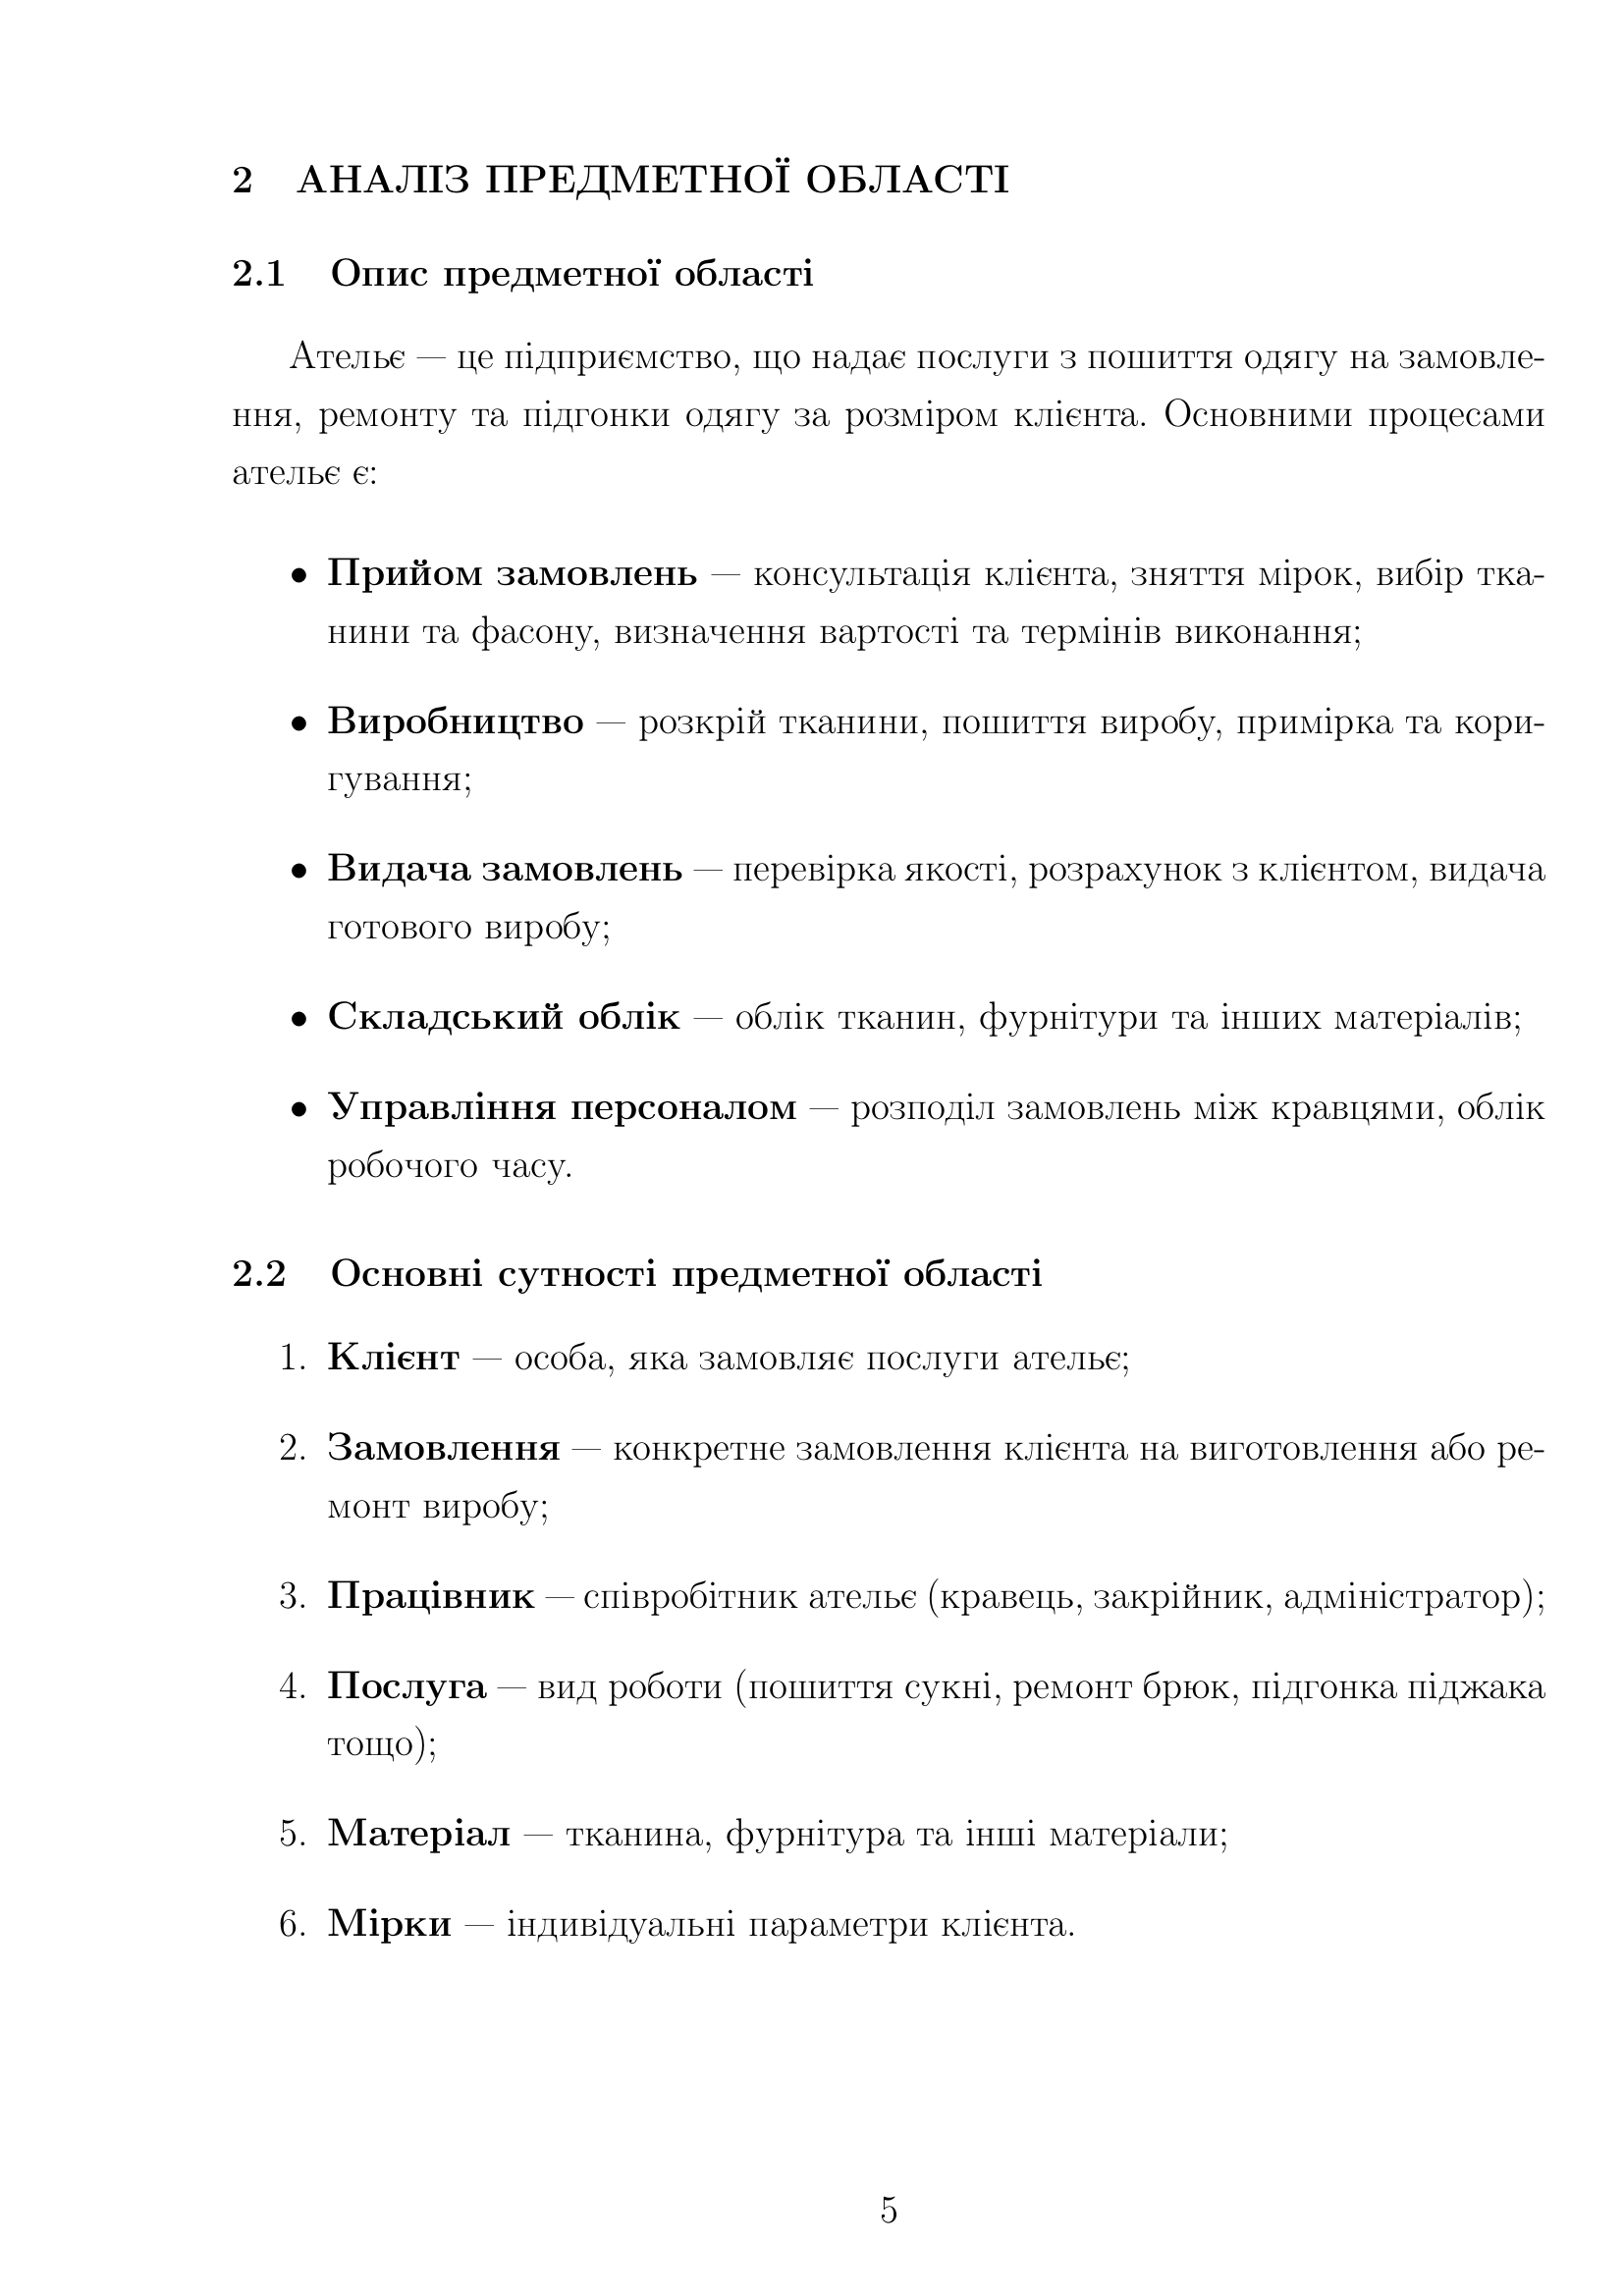
\includegraphics[width=0.85\textwidth]{diagrams/diagram-06.png}
\caption{Діаграма варіантів використання системи}
\end{figure}

\begin{figure}[h!]
\centering
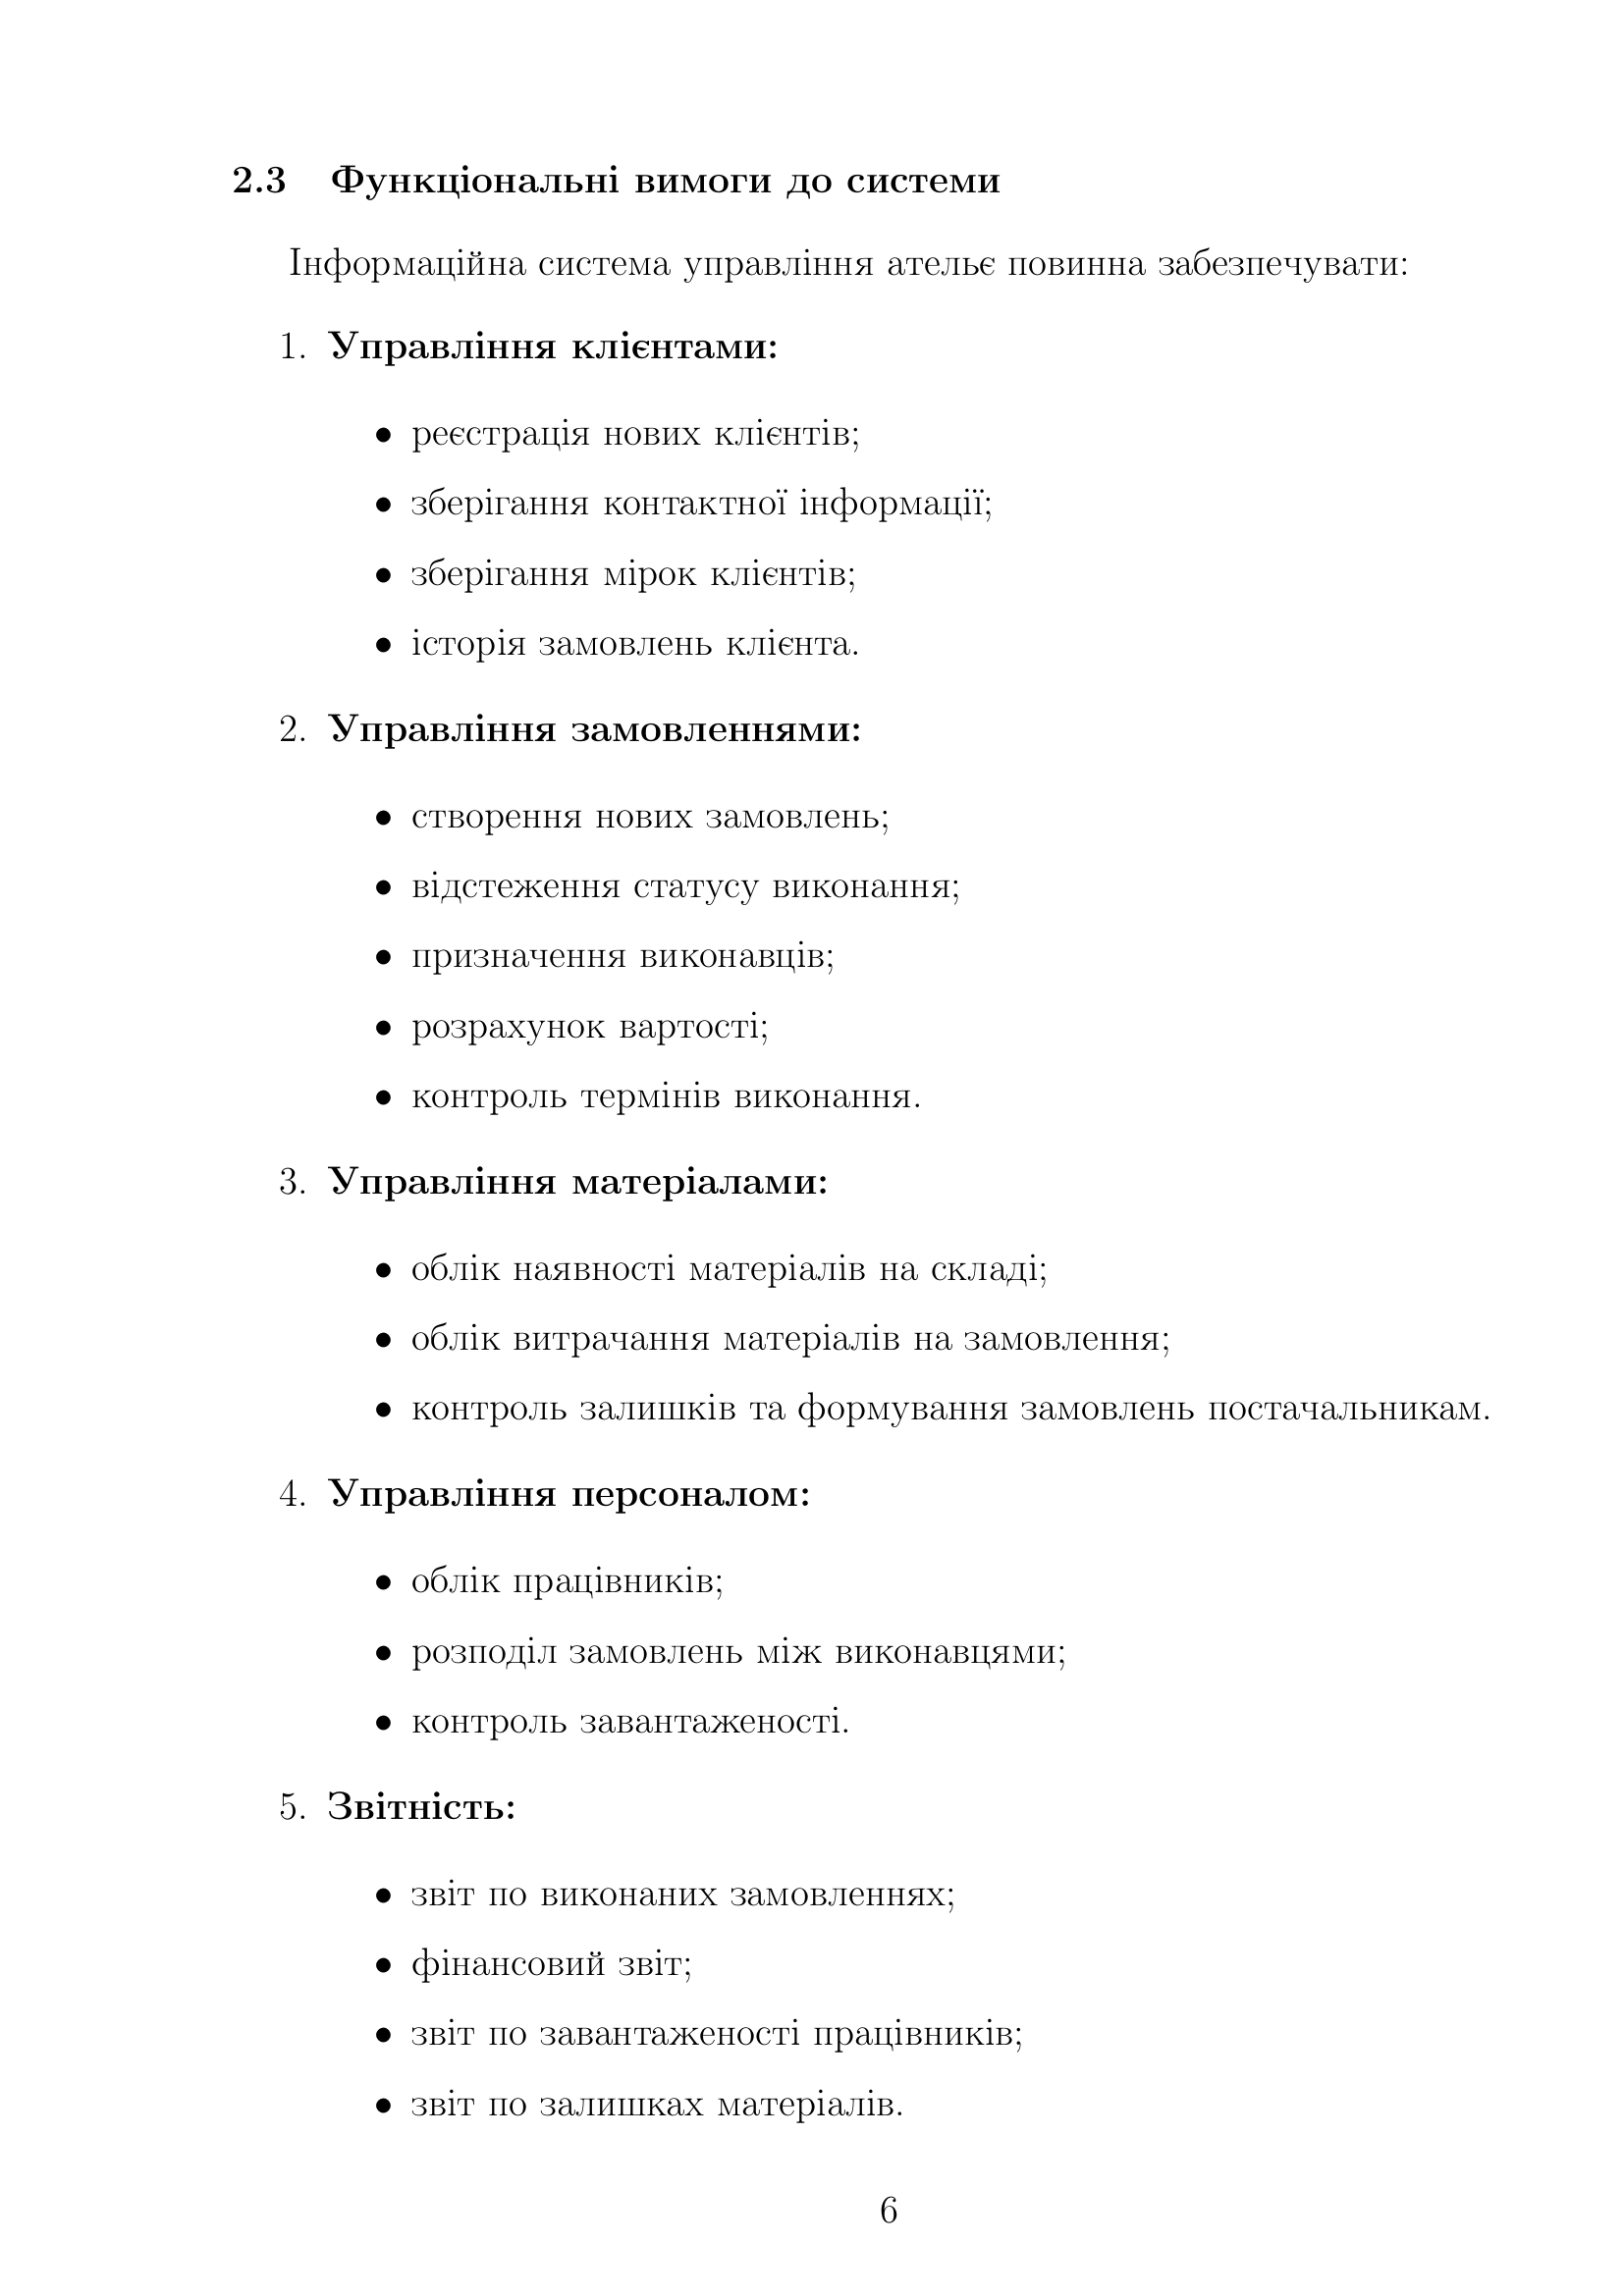
\includegraphics[width=0.85\textwidth]{diagrams/diagram-07.png}
\caption{Діаграма взаємодії компонентів}
\end{figure}

\newpage

\begin{figure}[h!]
\centering
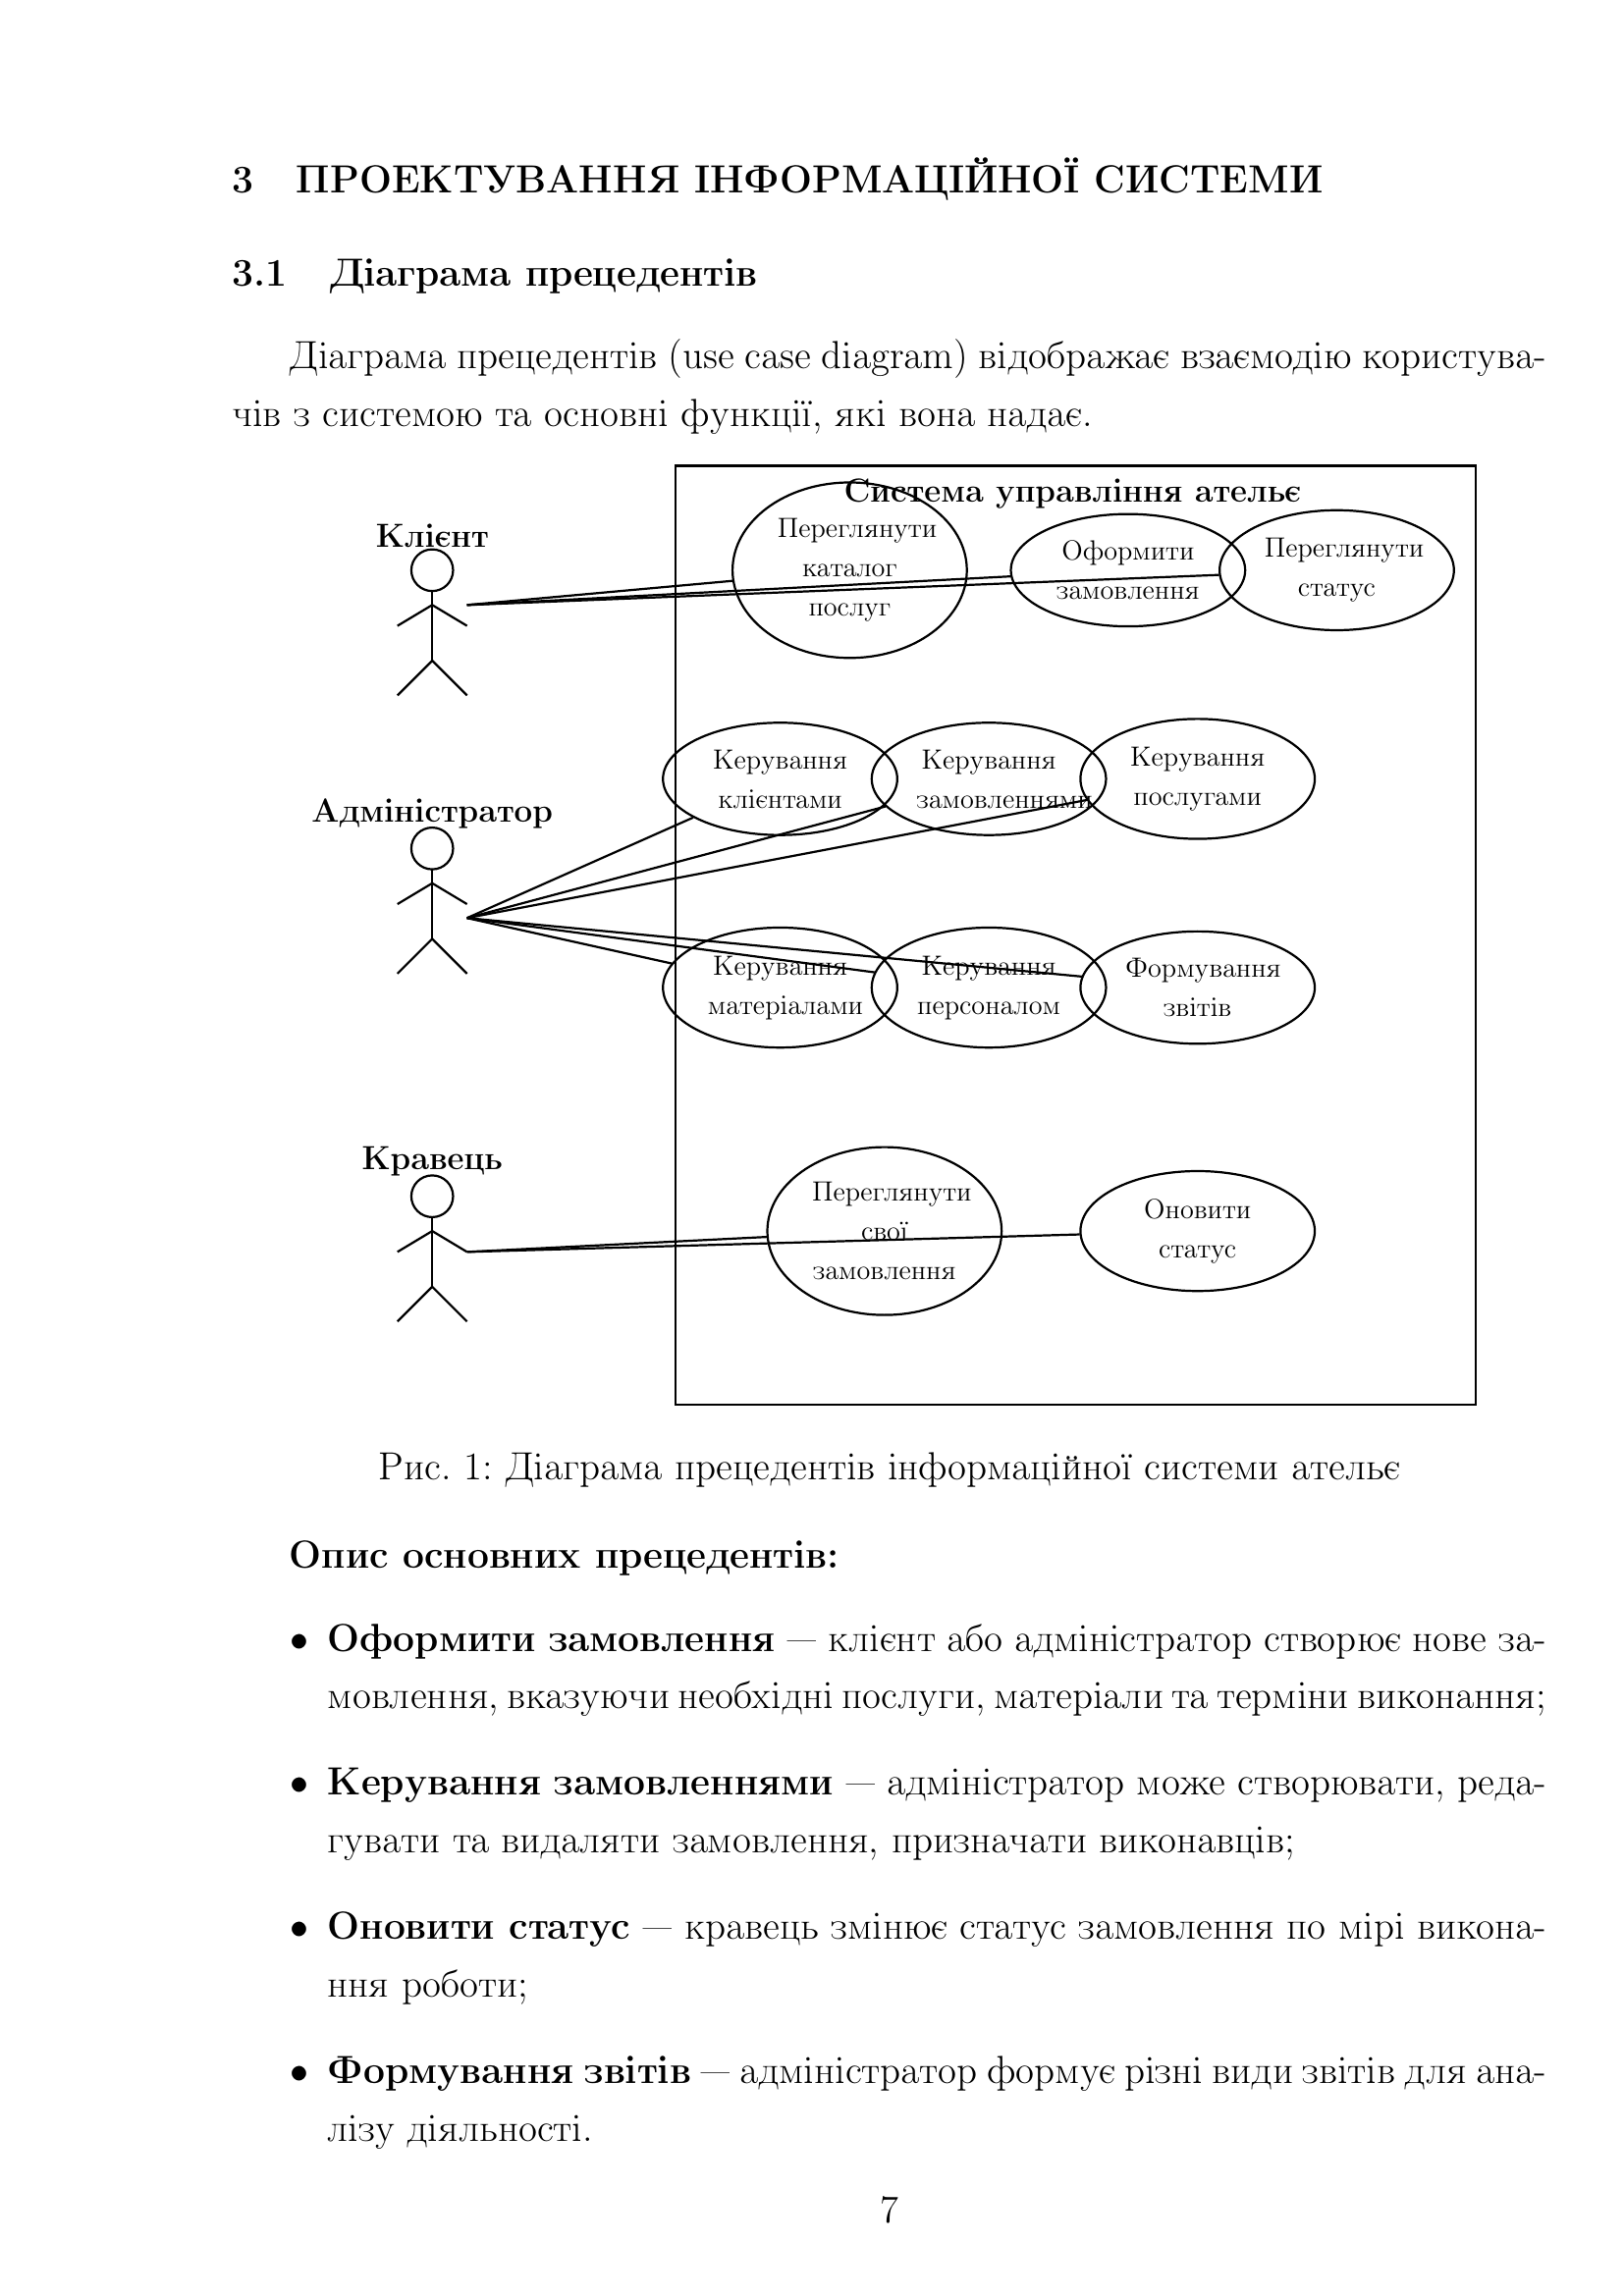
\includegraphics[width=0.85\textwidth]{diagrams/diagram-08.png}
\caption{Діаграма потоків даних}
\end{figure}

\begin{figure}[h!]
\centering
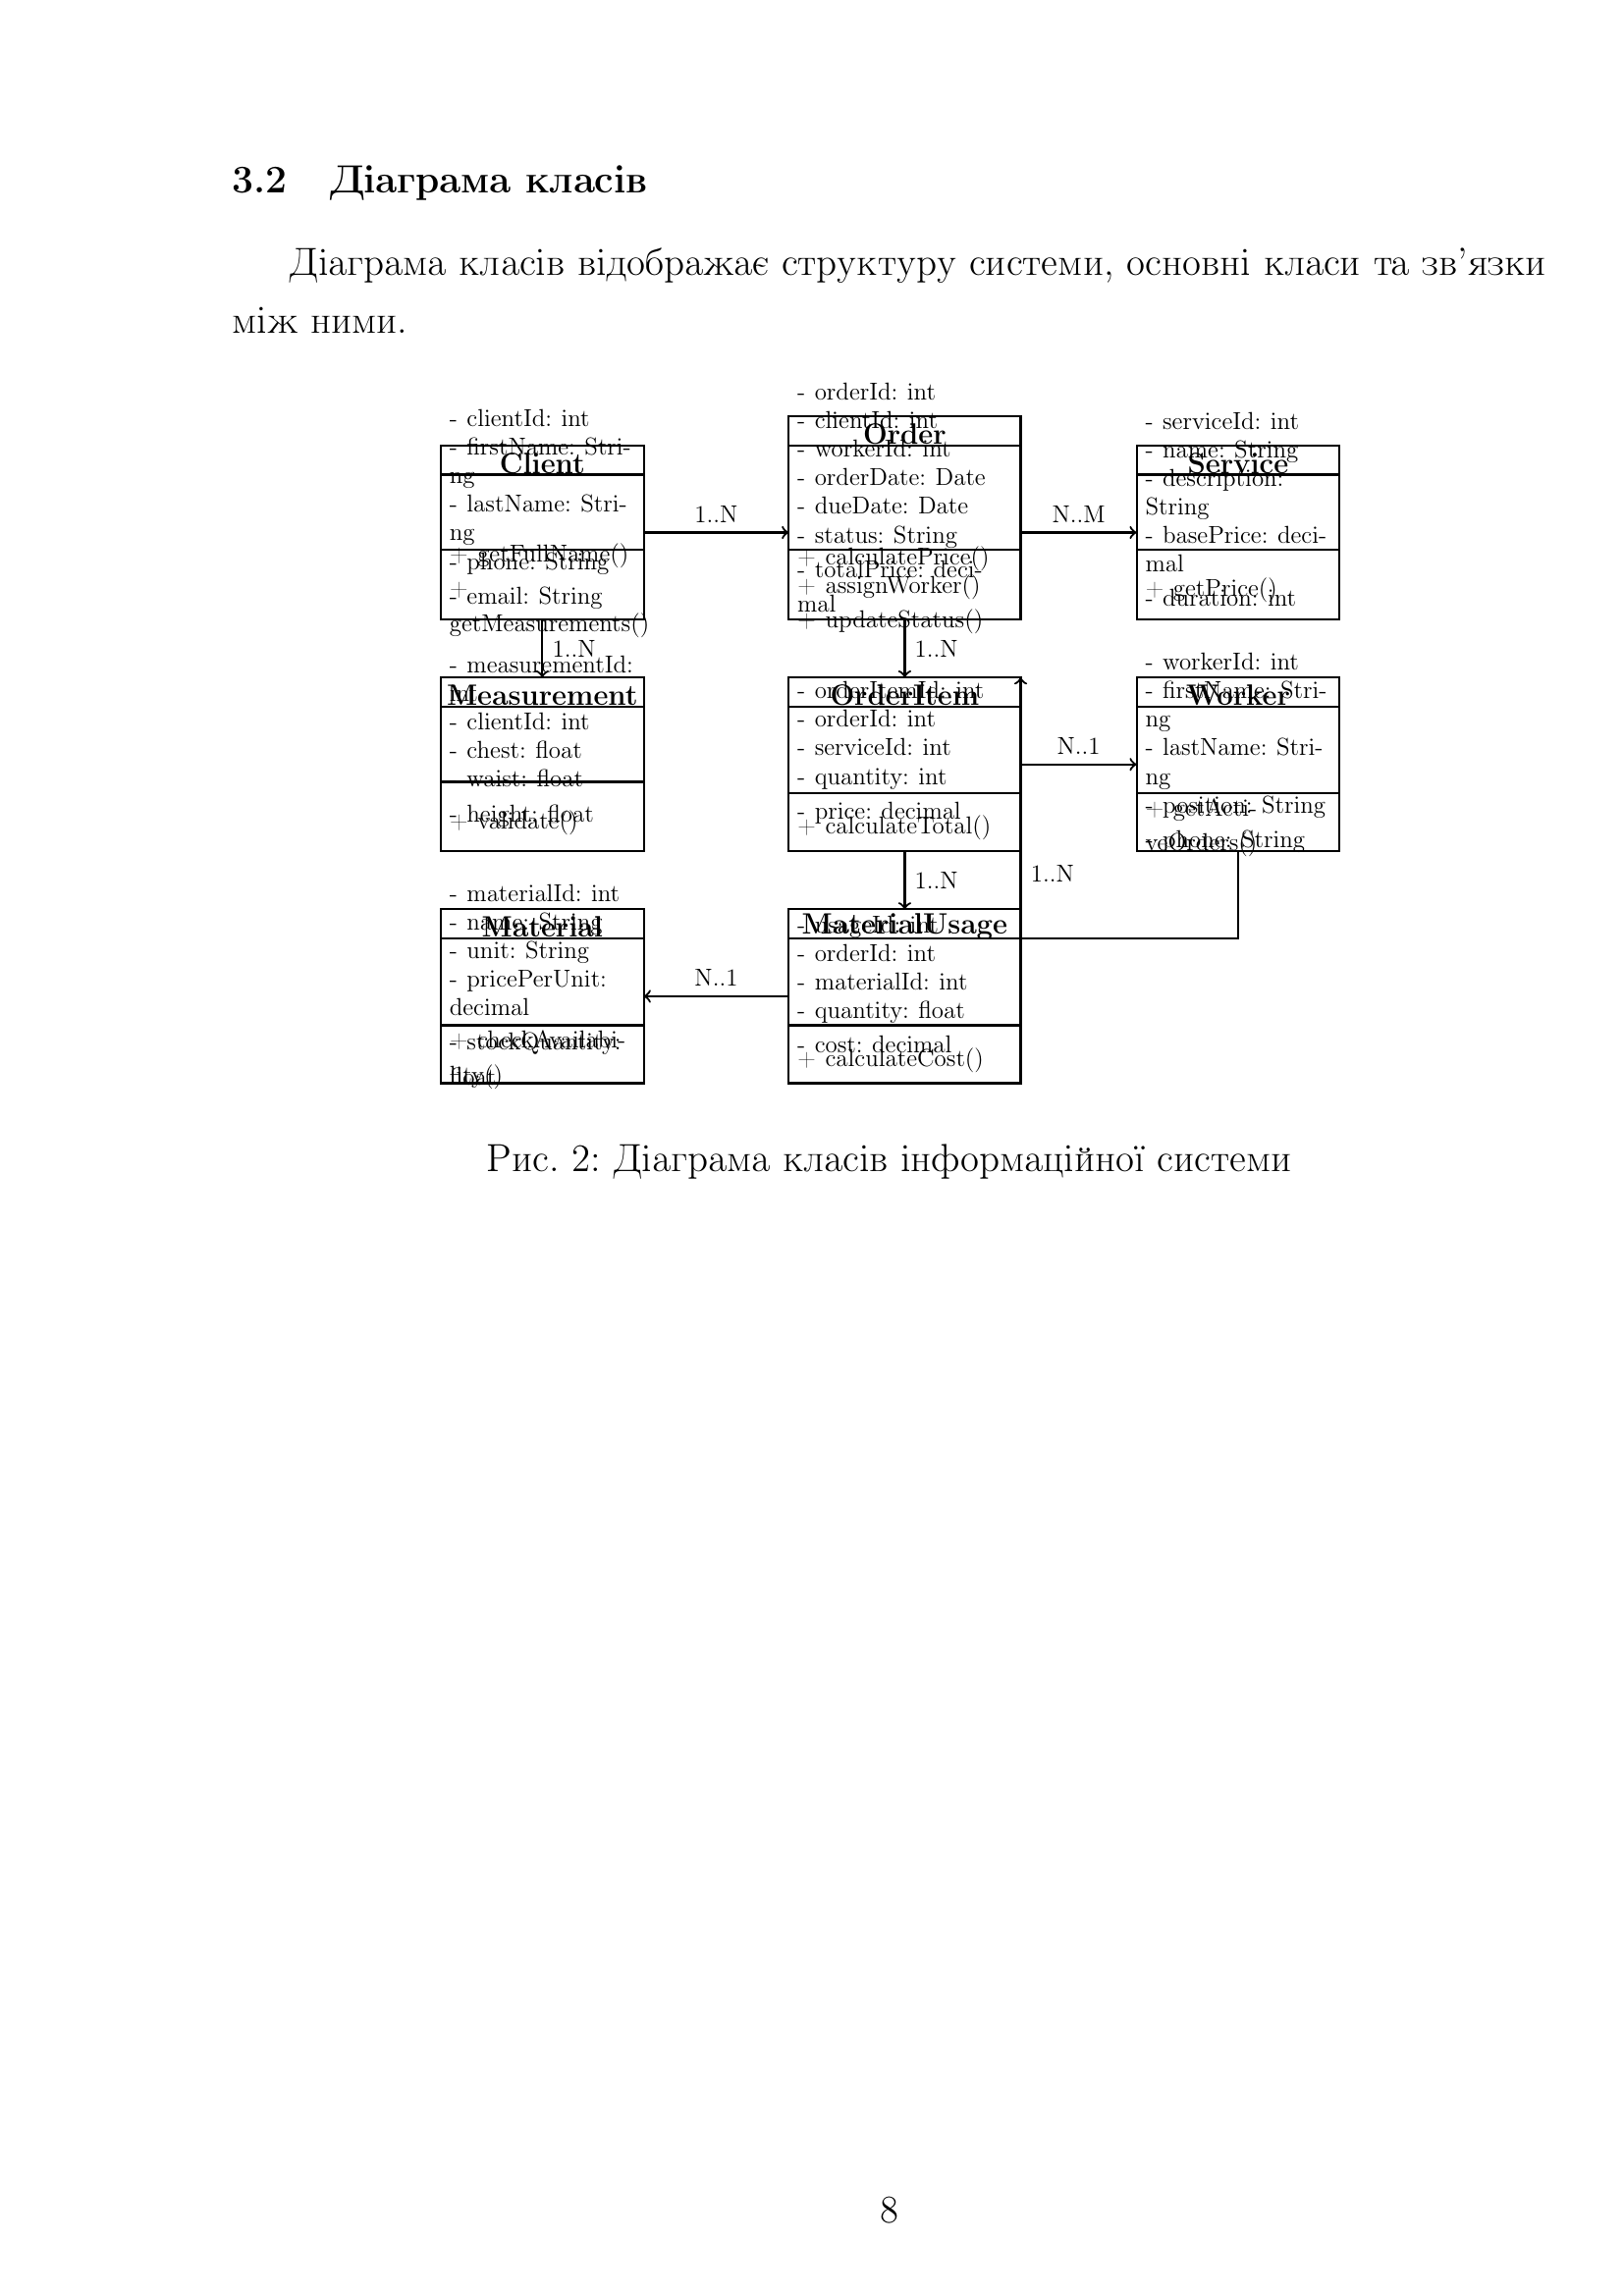
\includegraphics[width=0.85\textwidth]{diagrams/diagram-09.png}
\caption{Діаграма бізнес-процесів}
\end{figure}

\newpage

\begin{figure}[h!]
\centering
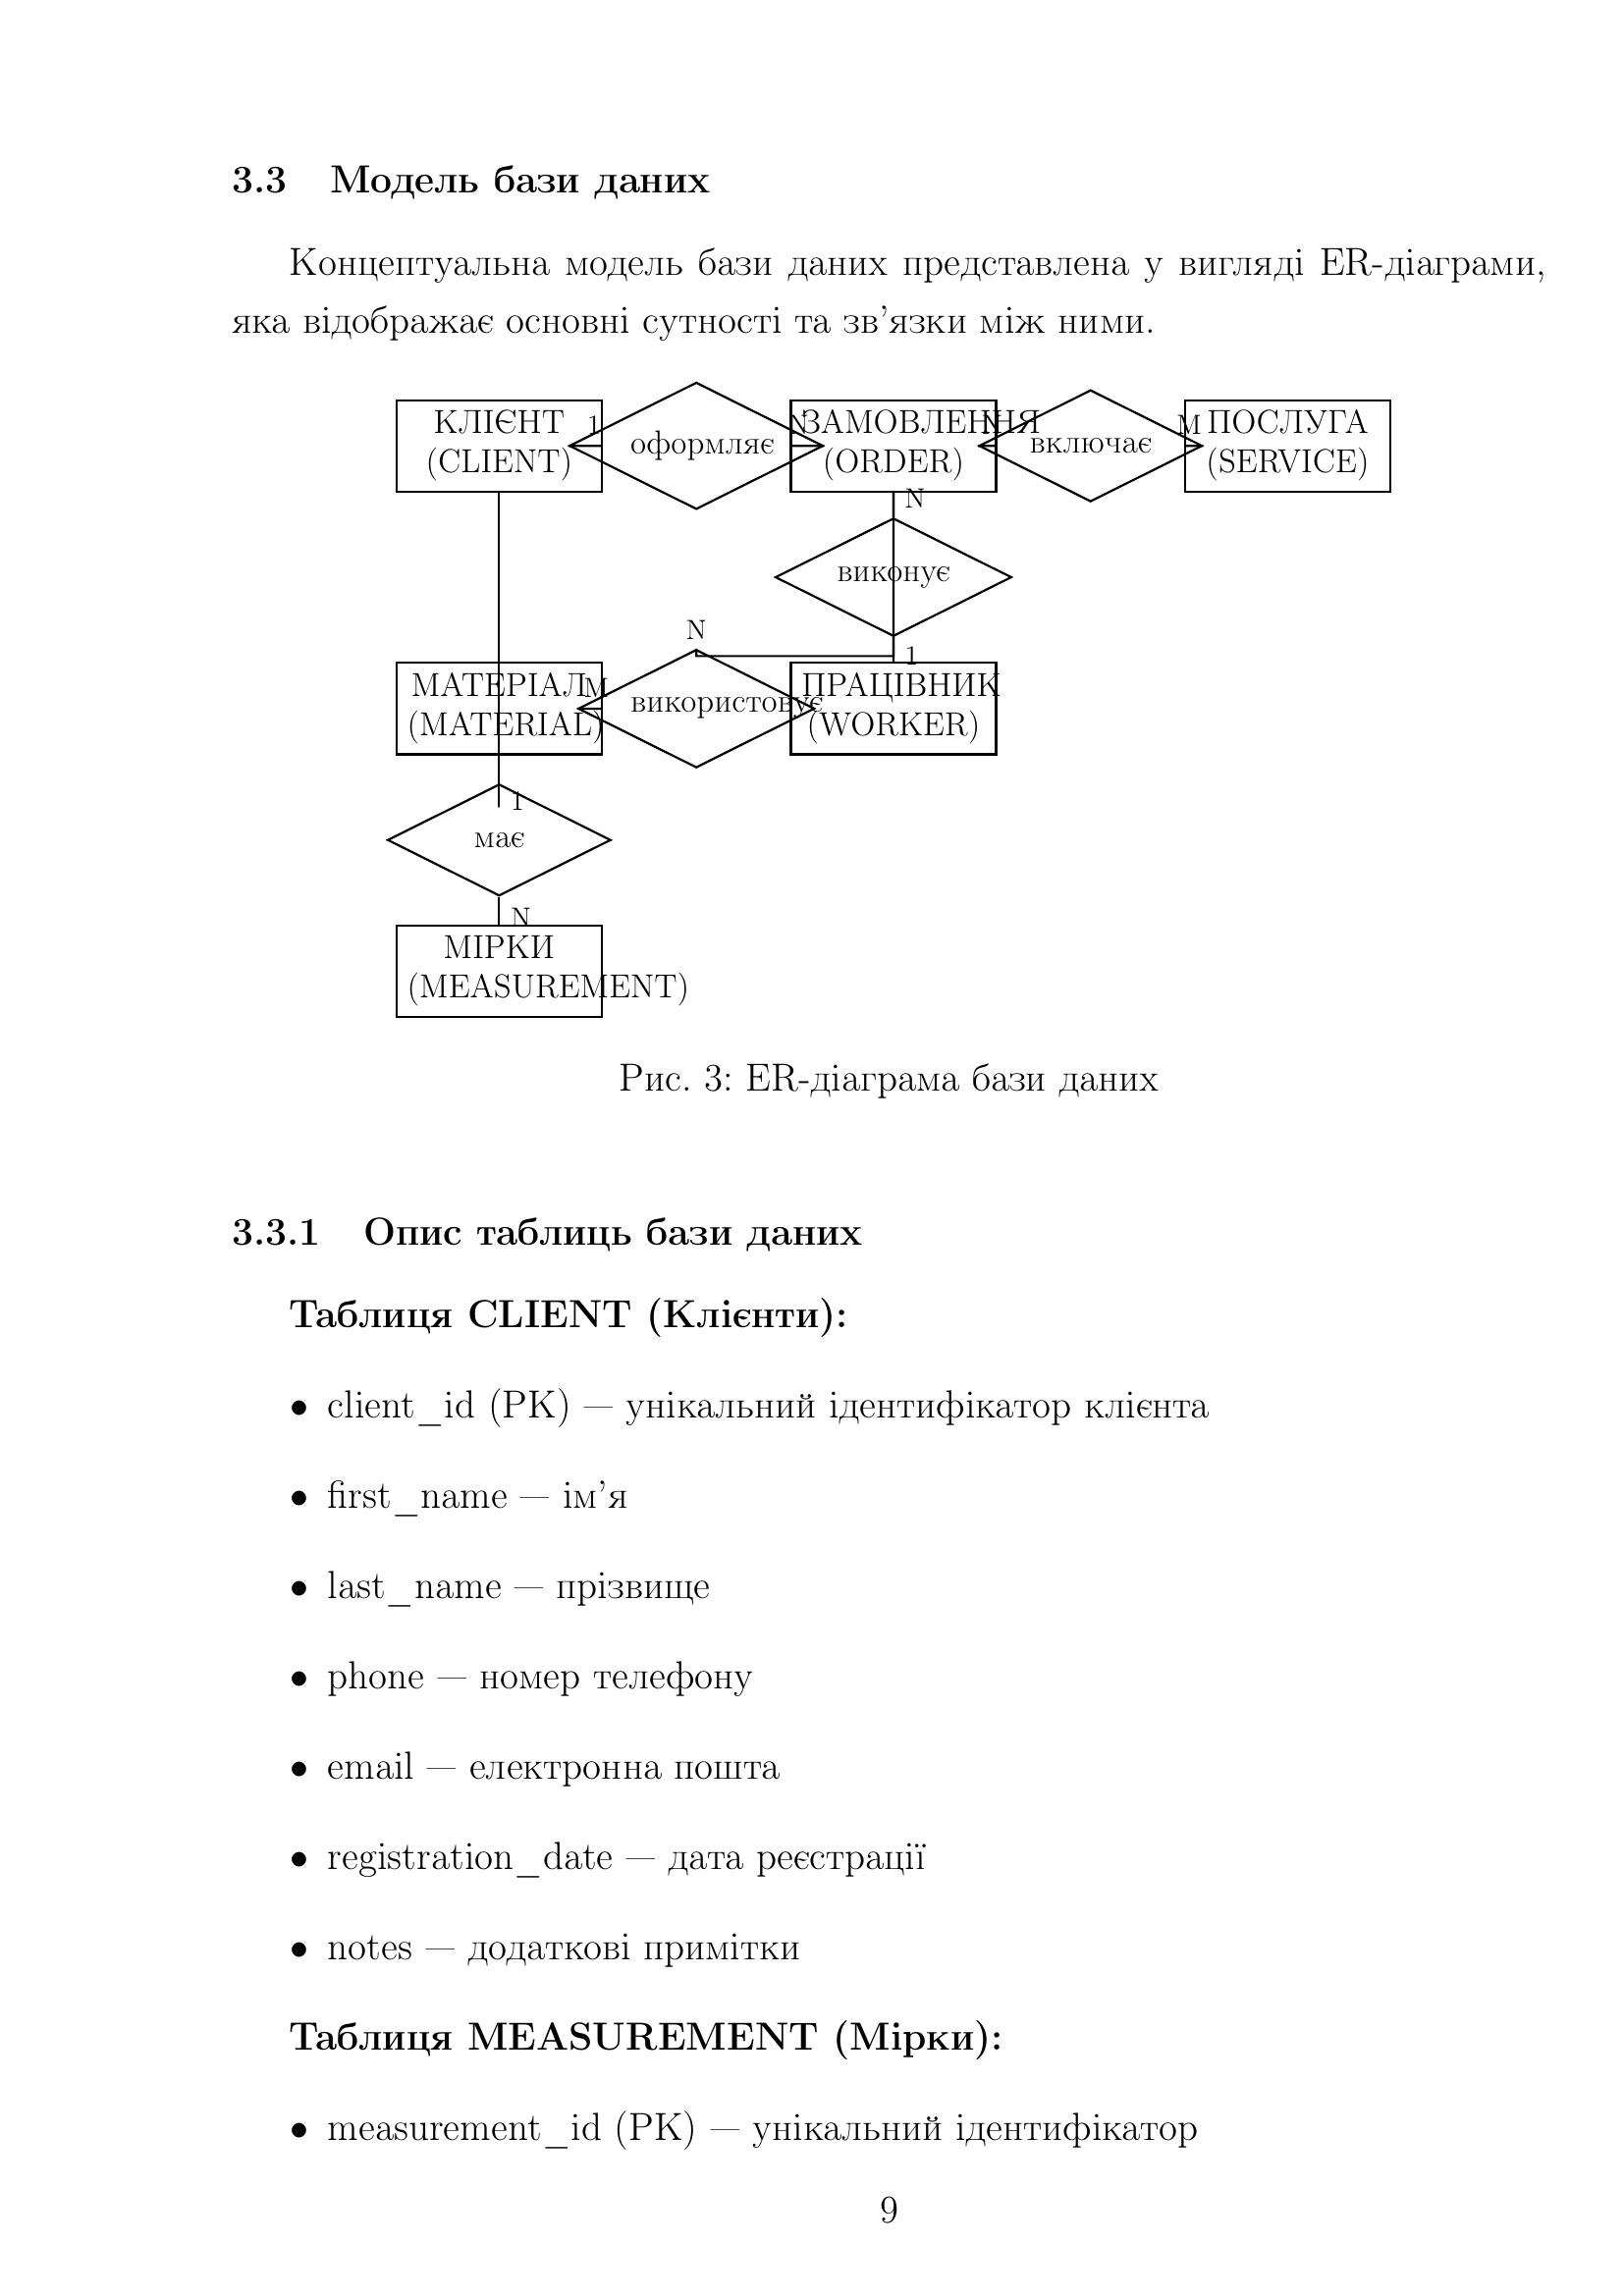
\includegraphics[width=0.85\textwidth]{diagrams/diagram-10.png}
\caption{Діаграма архітектури додатку}
\end{figure}

\begin{figure}[h!]
\centering
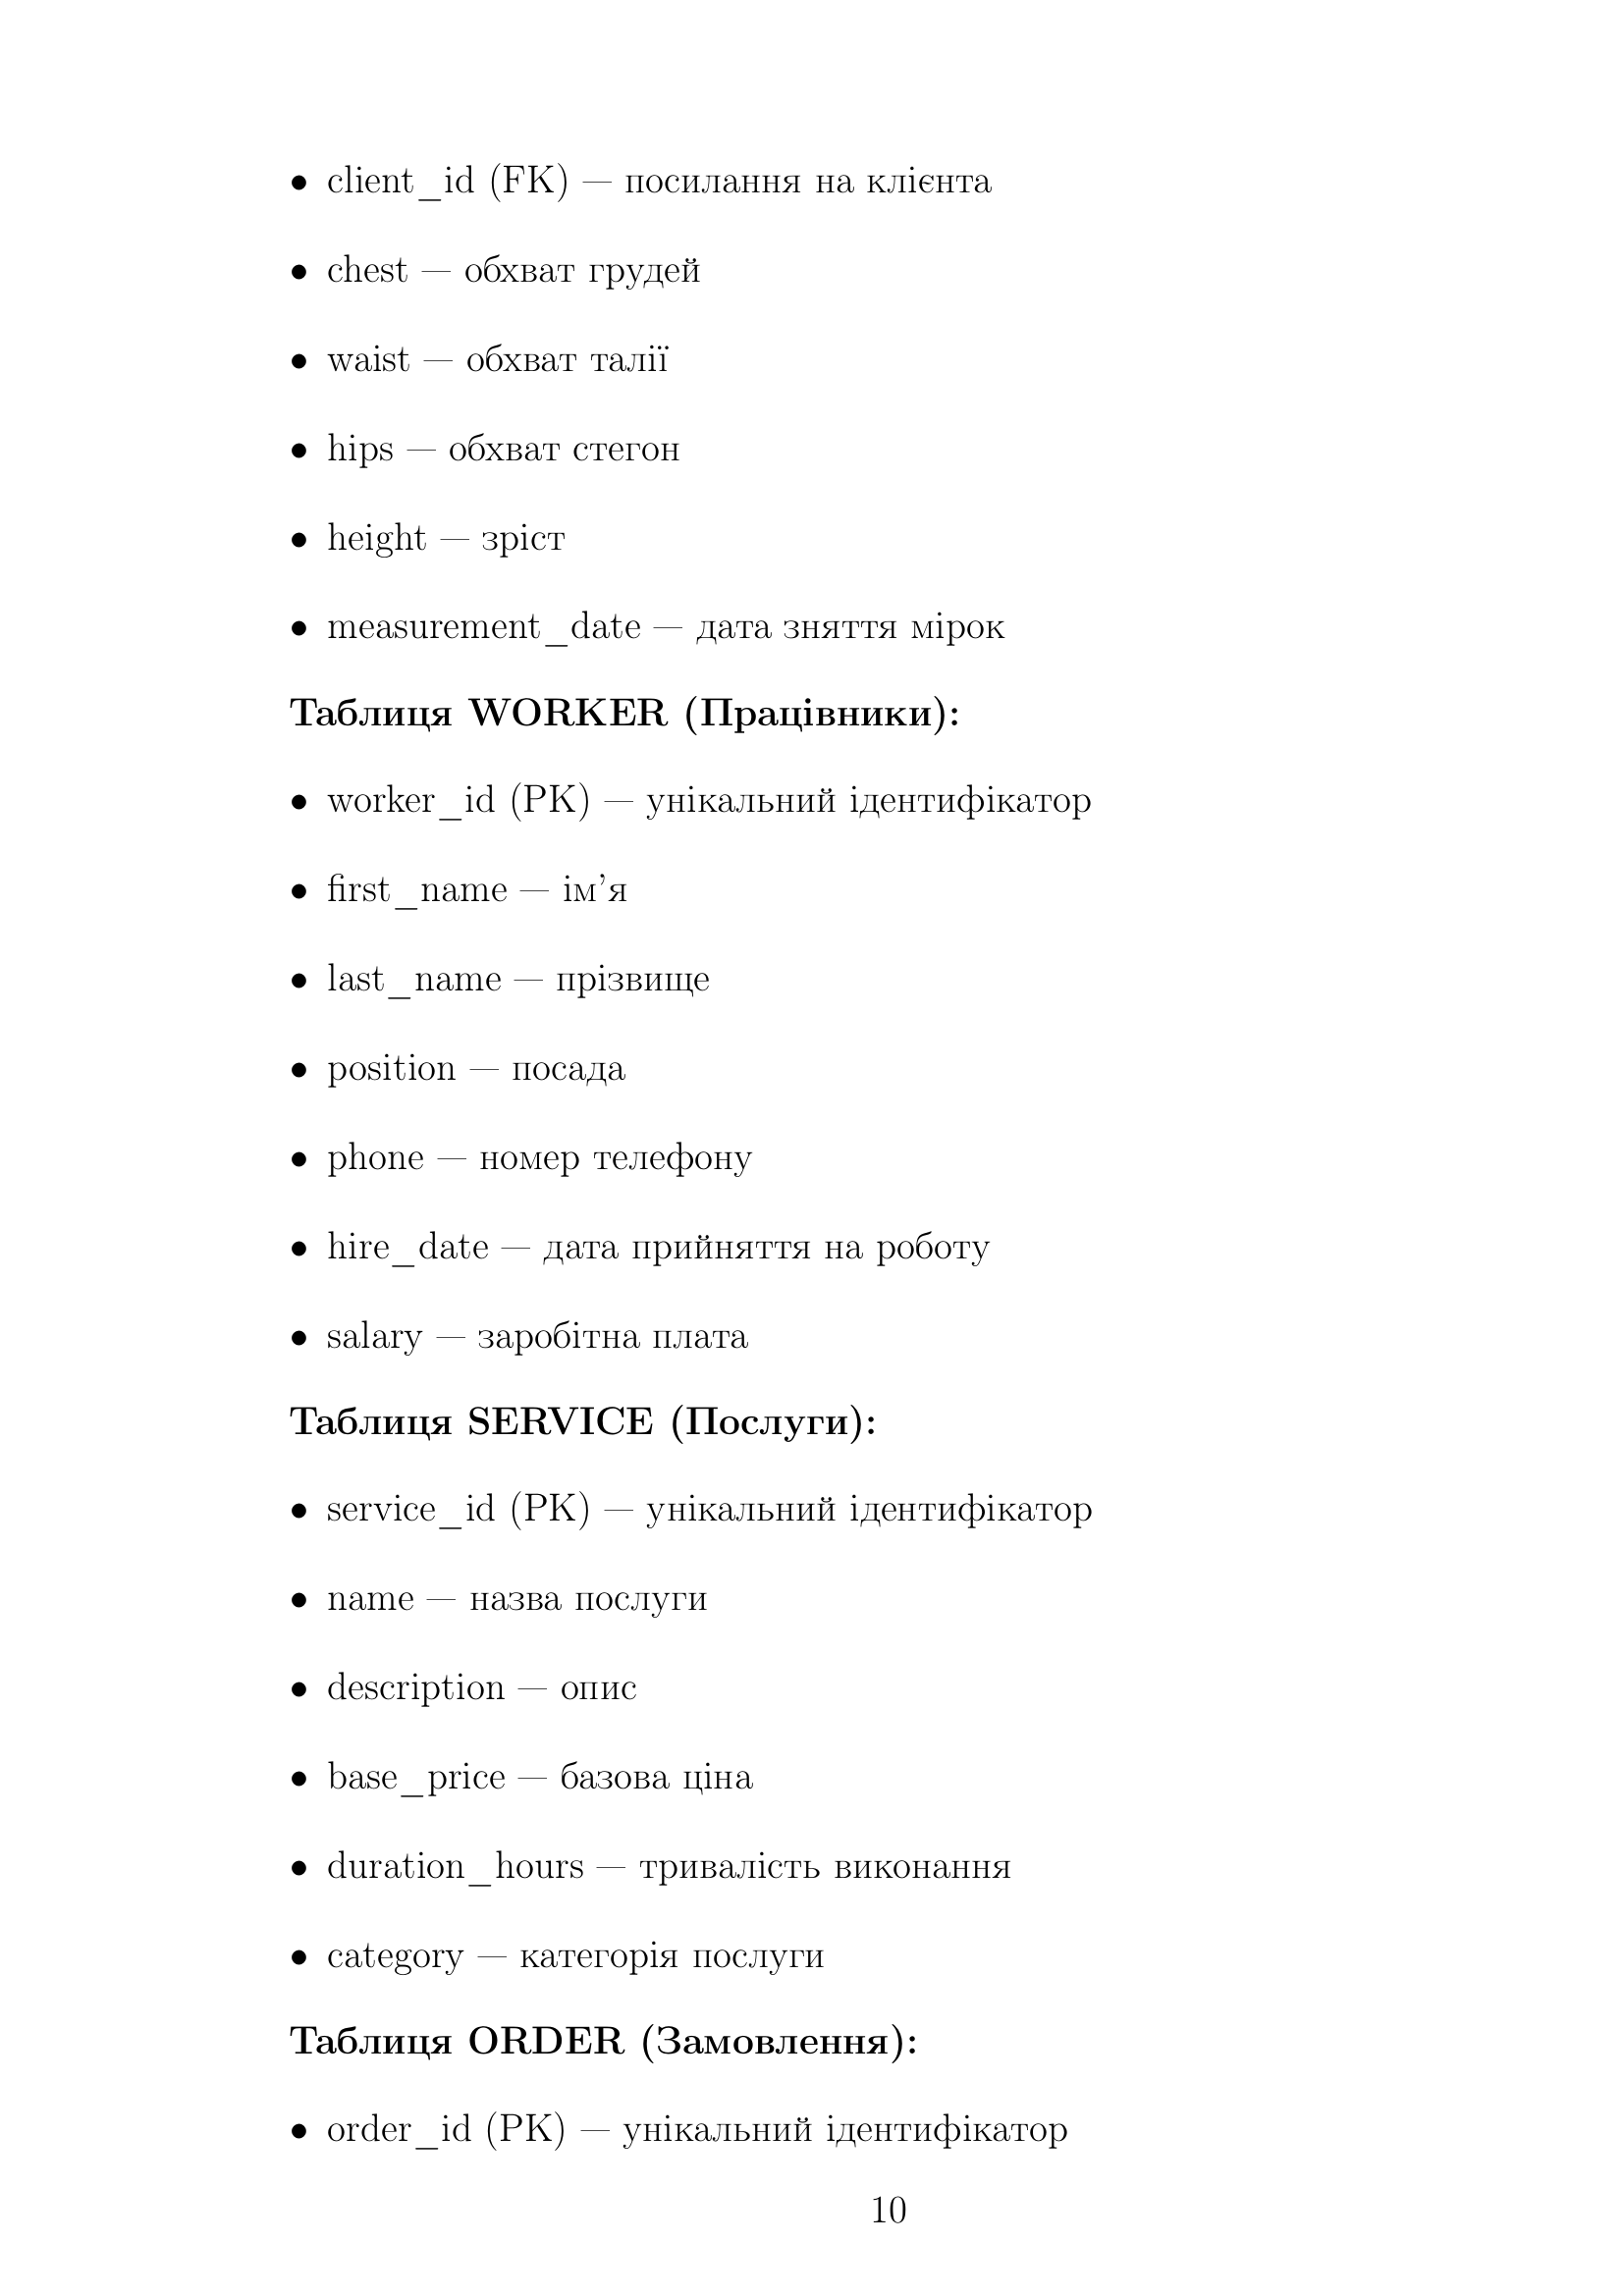
\includegraphics[width=0.85\textwidth]{diagrams/diagram-11.png}
\caption{Діаграма безпеки системи}
\end{figure}

\newpage

\begin{figure}[h!]
\centering
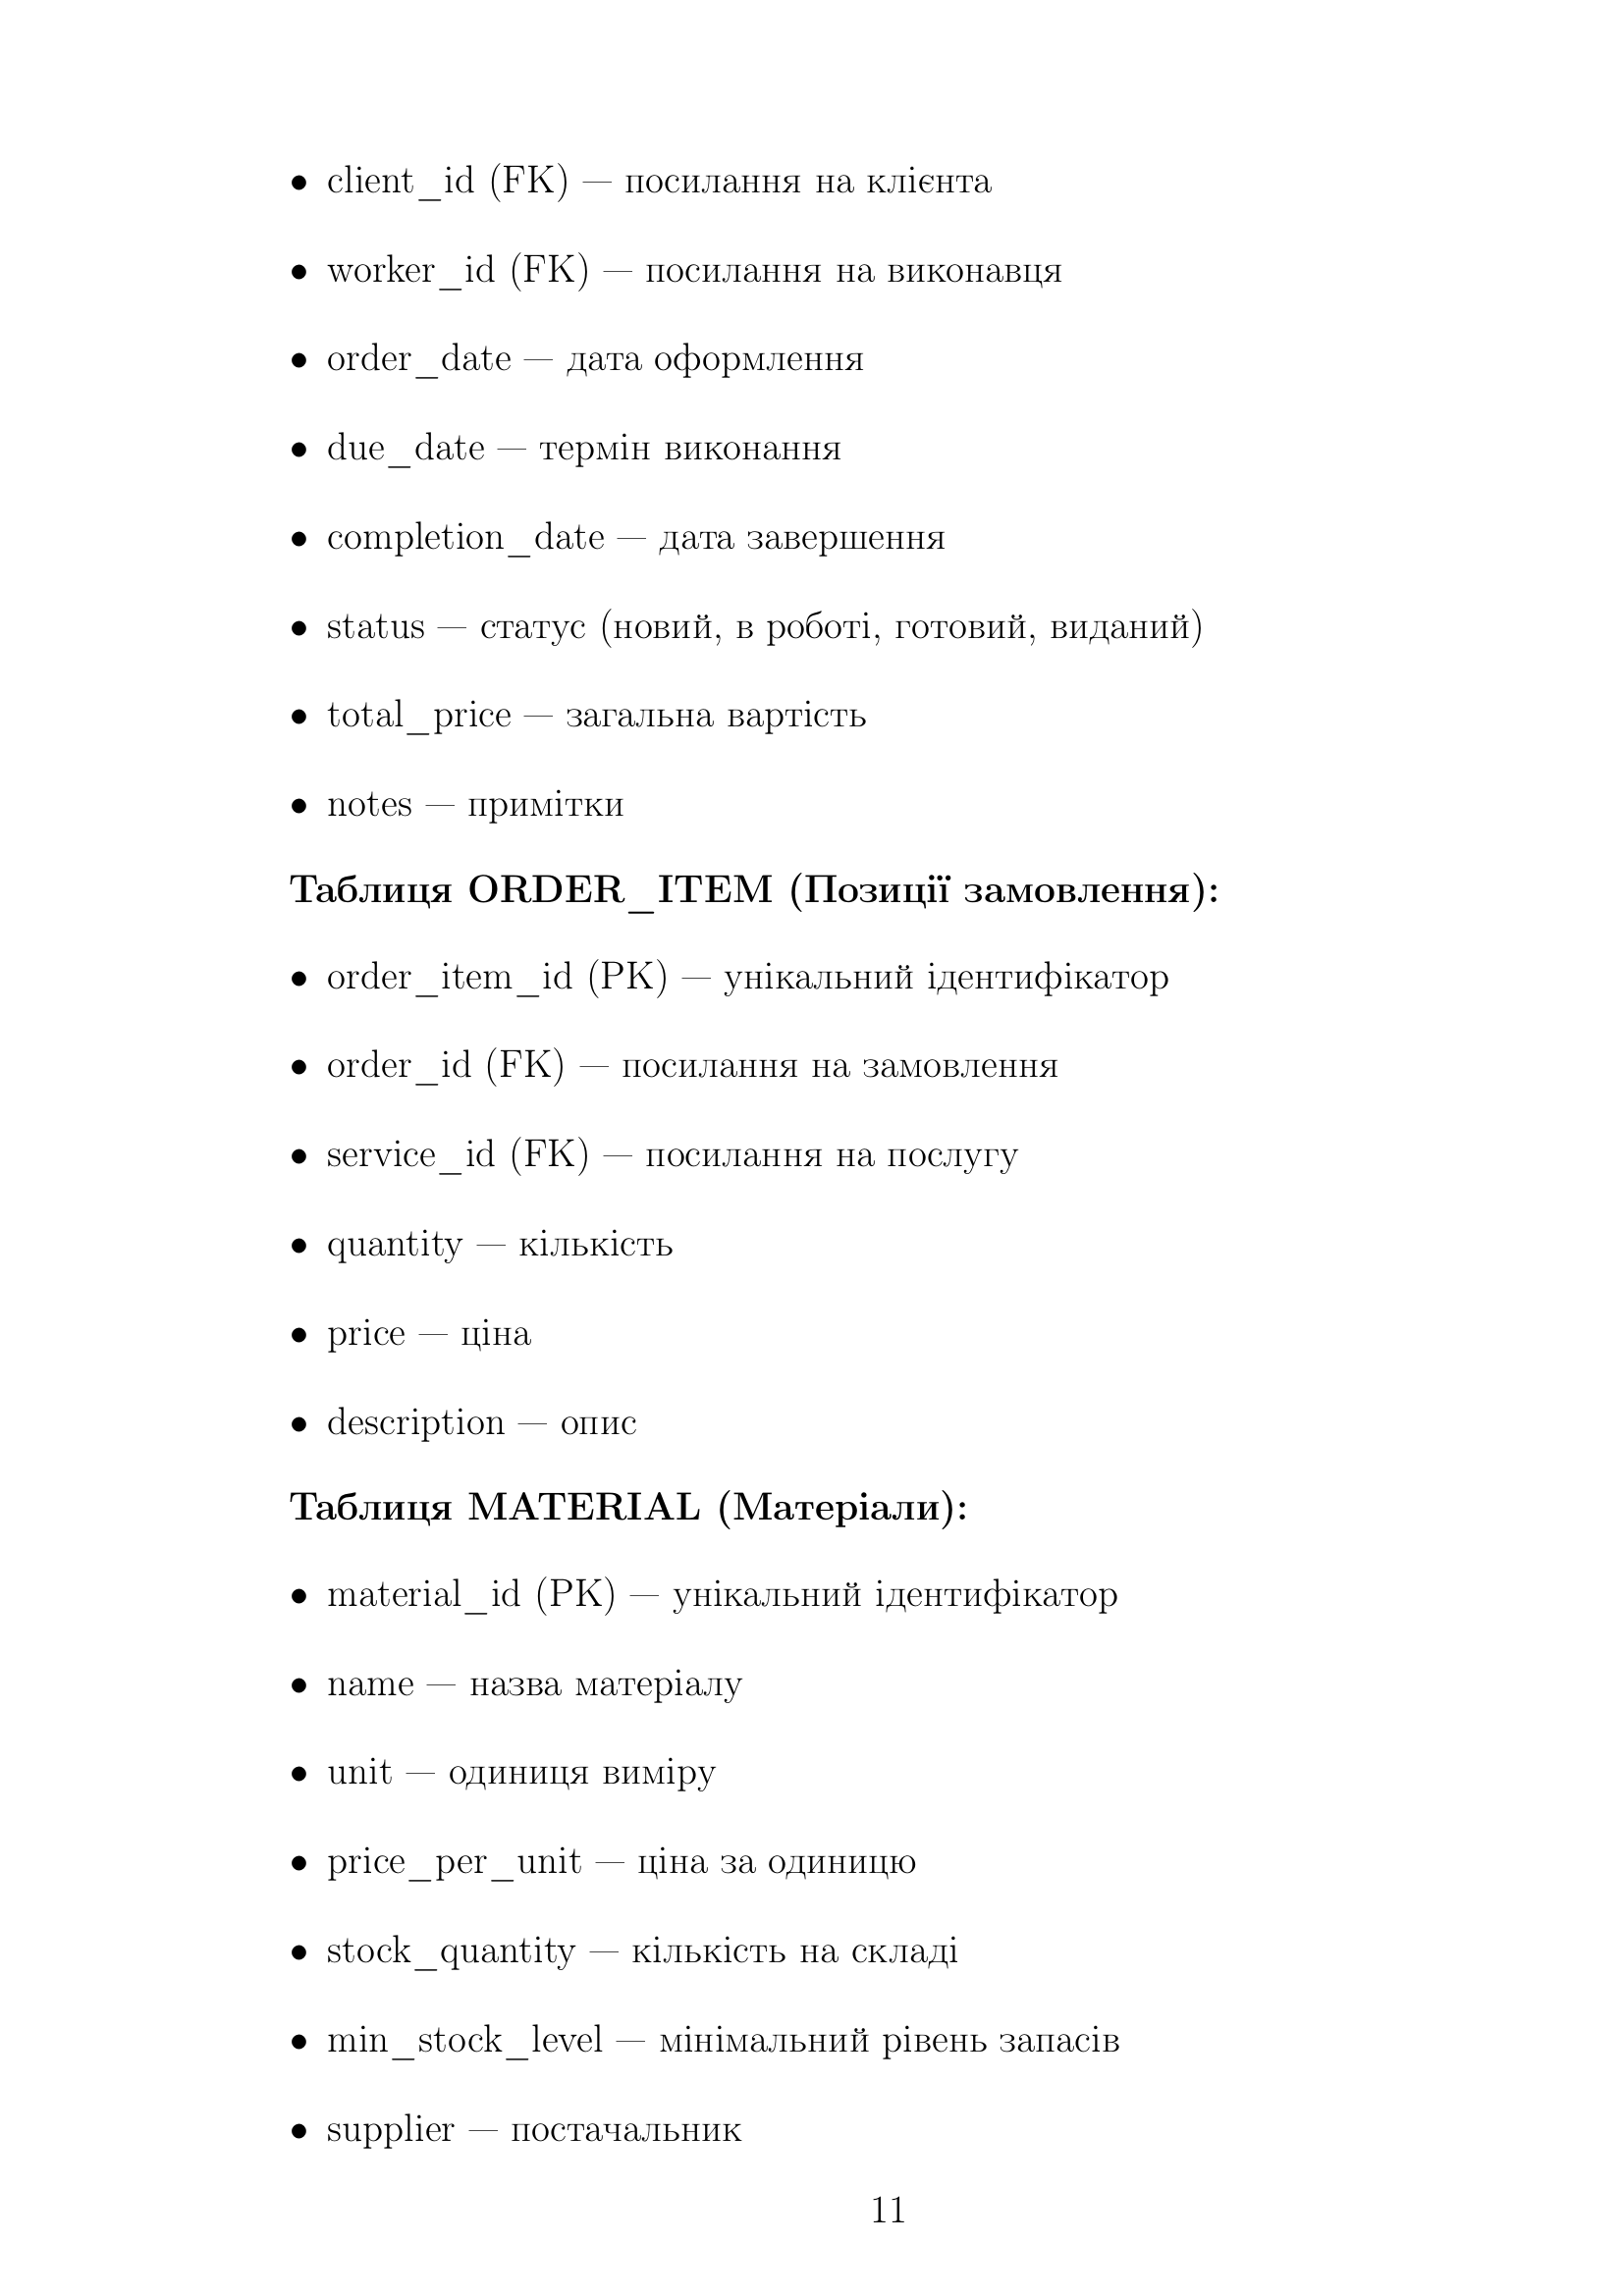
\includegraphics[width=0.85\textwidth]{diagrams/diagram-12.png}
\caption{Діаграма інтеграції з зовнішніми системами}
\end{figure}

\begin{figure}[h!]
\centering
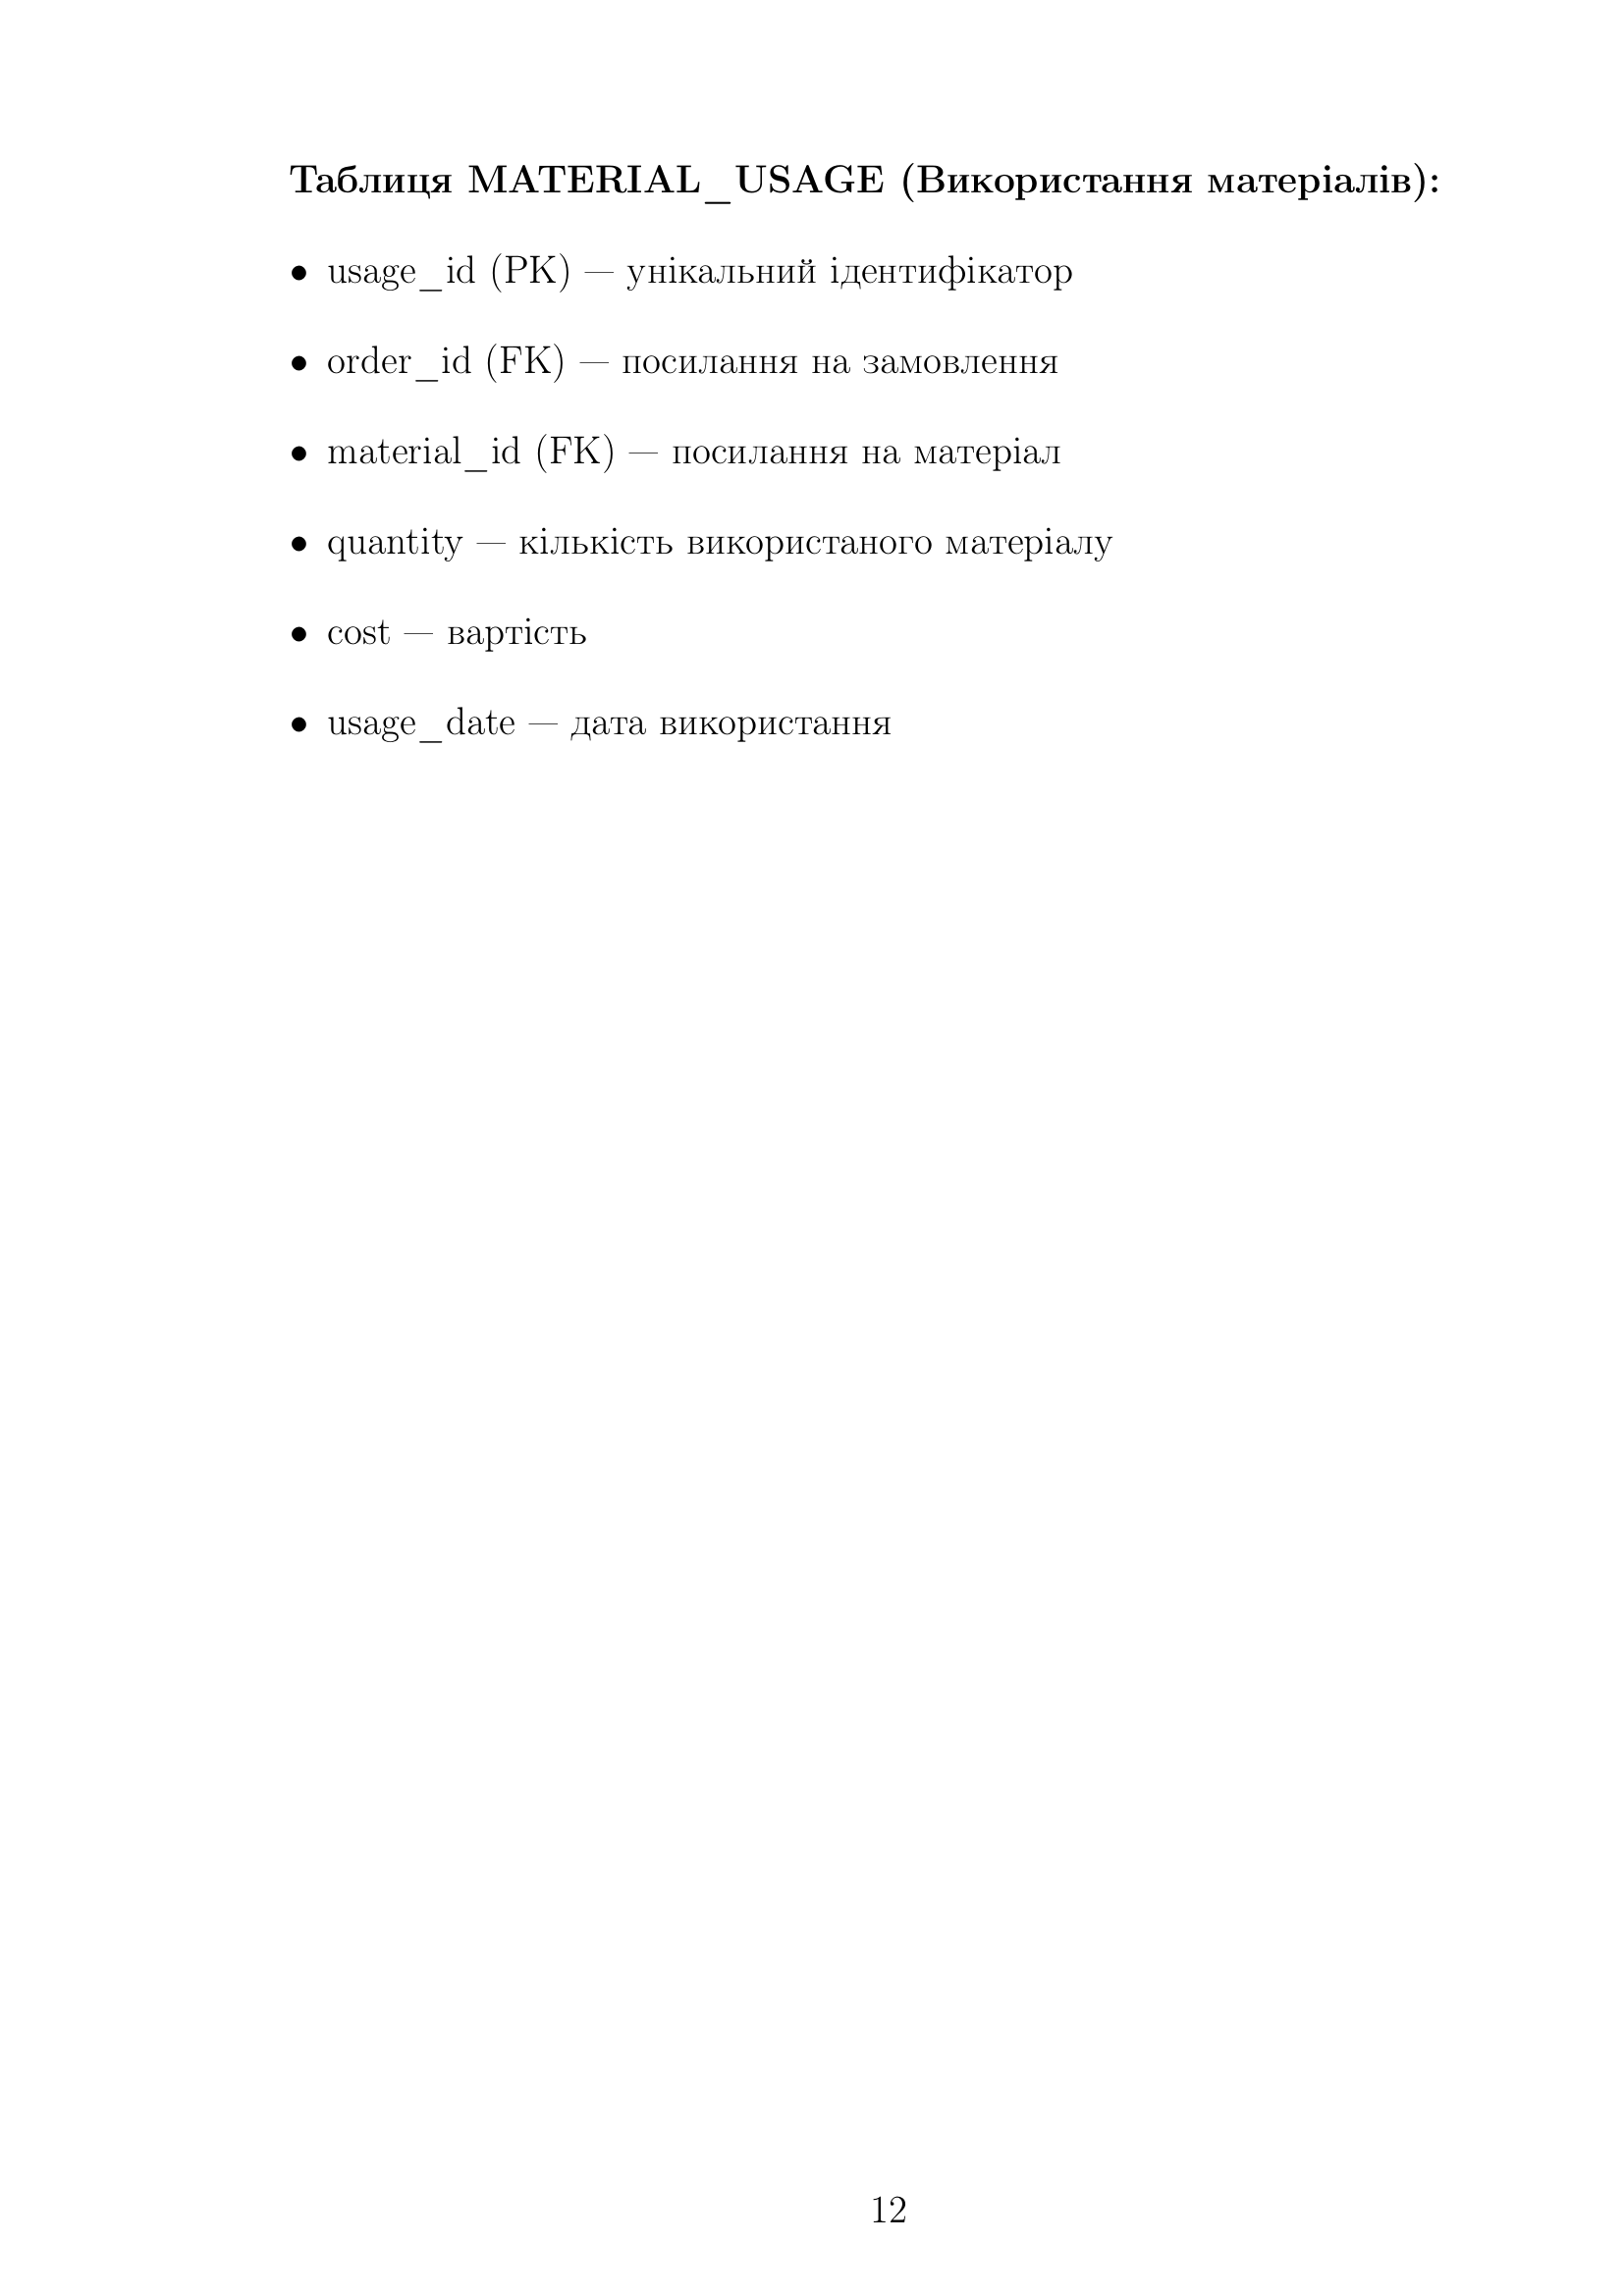
\includegraphics[width=0.85\textwidth]{diagrams/diagram-13.png}
\caption{Діаграма управління даними}
\end{figure}

\newpage

\begin{figure}[h!]
\centering
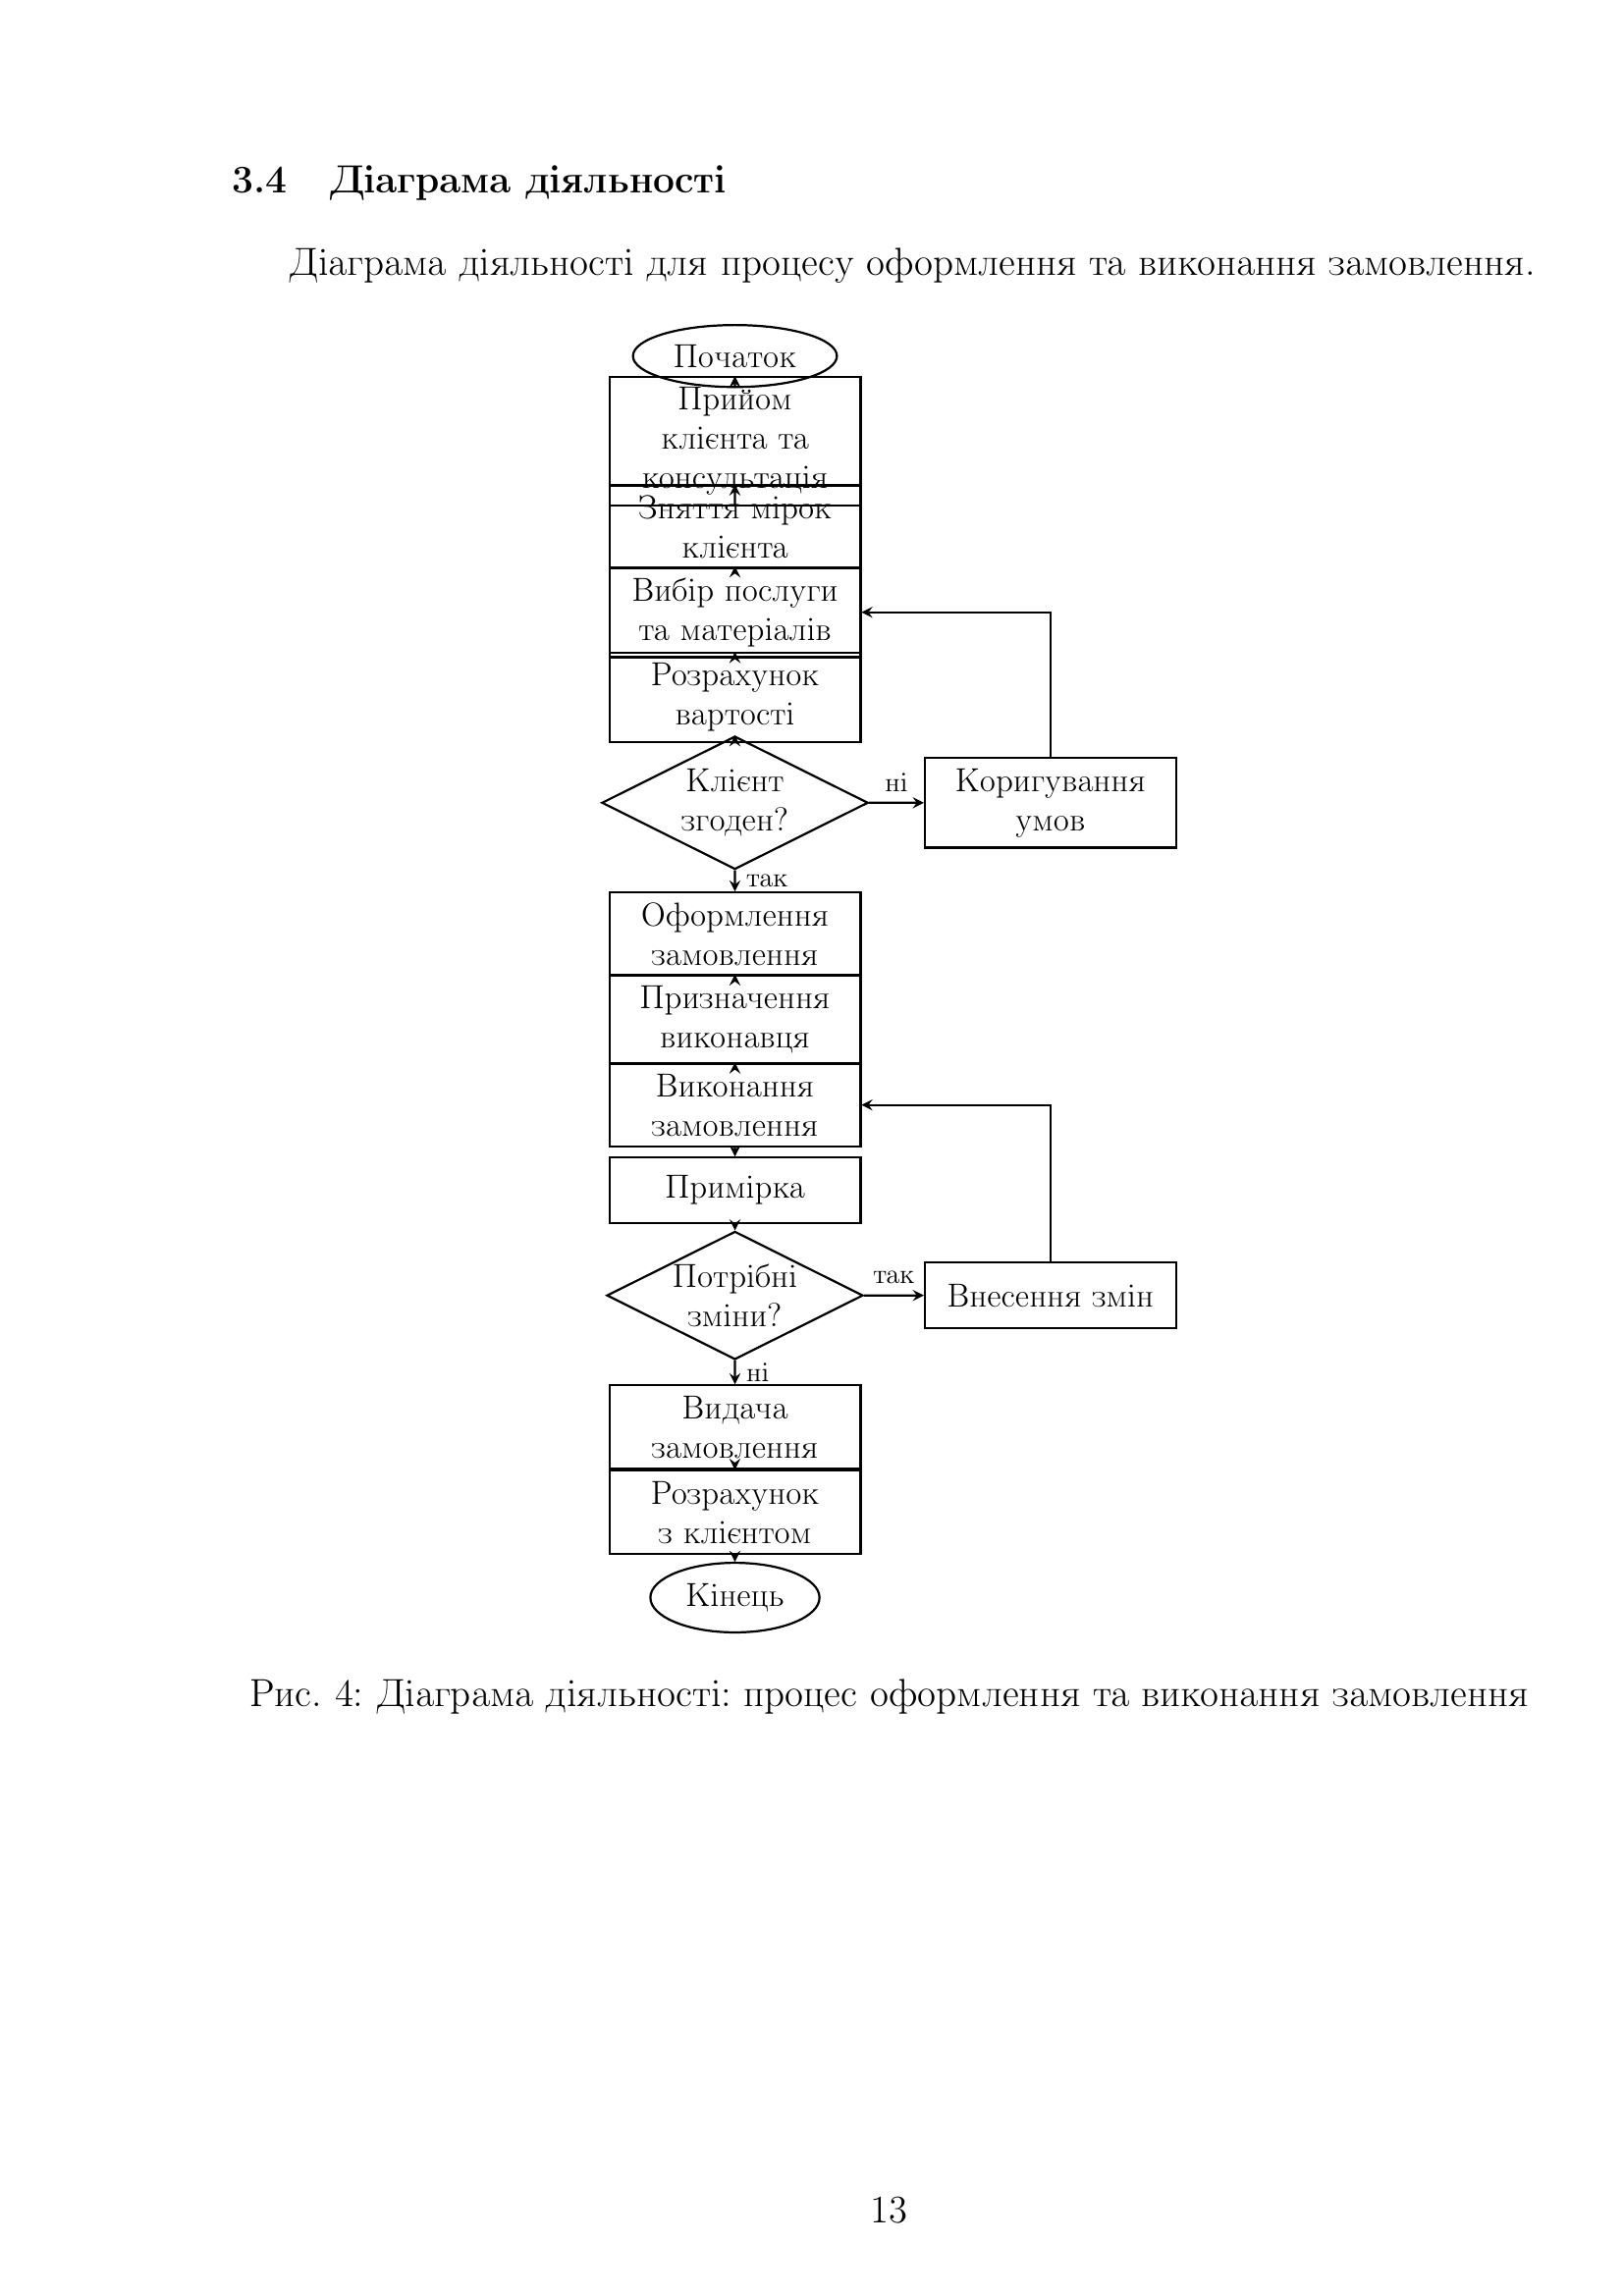
\includegraphics[width=0.85\textwidth]{diagrams/diagram-14.png}
\caption{Діаграма звітності системи}
\end{figure}

\begin{figure}[h!]
\centering
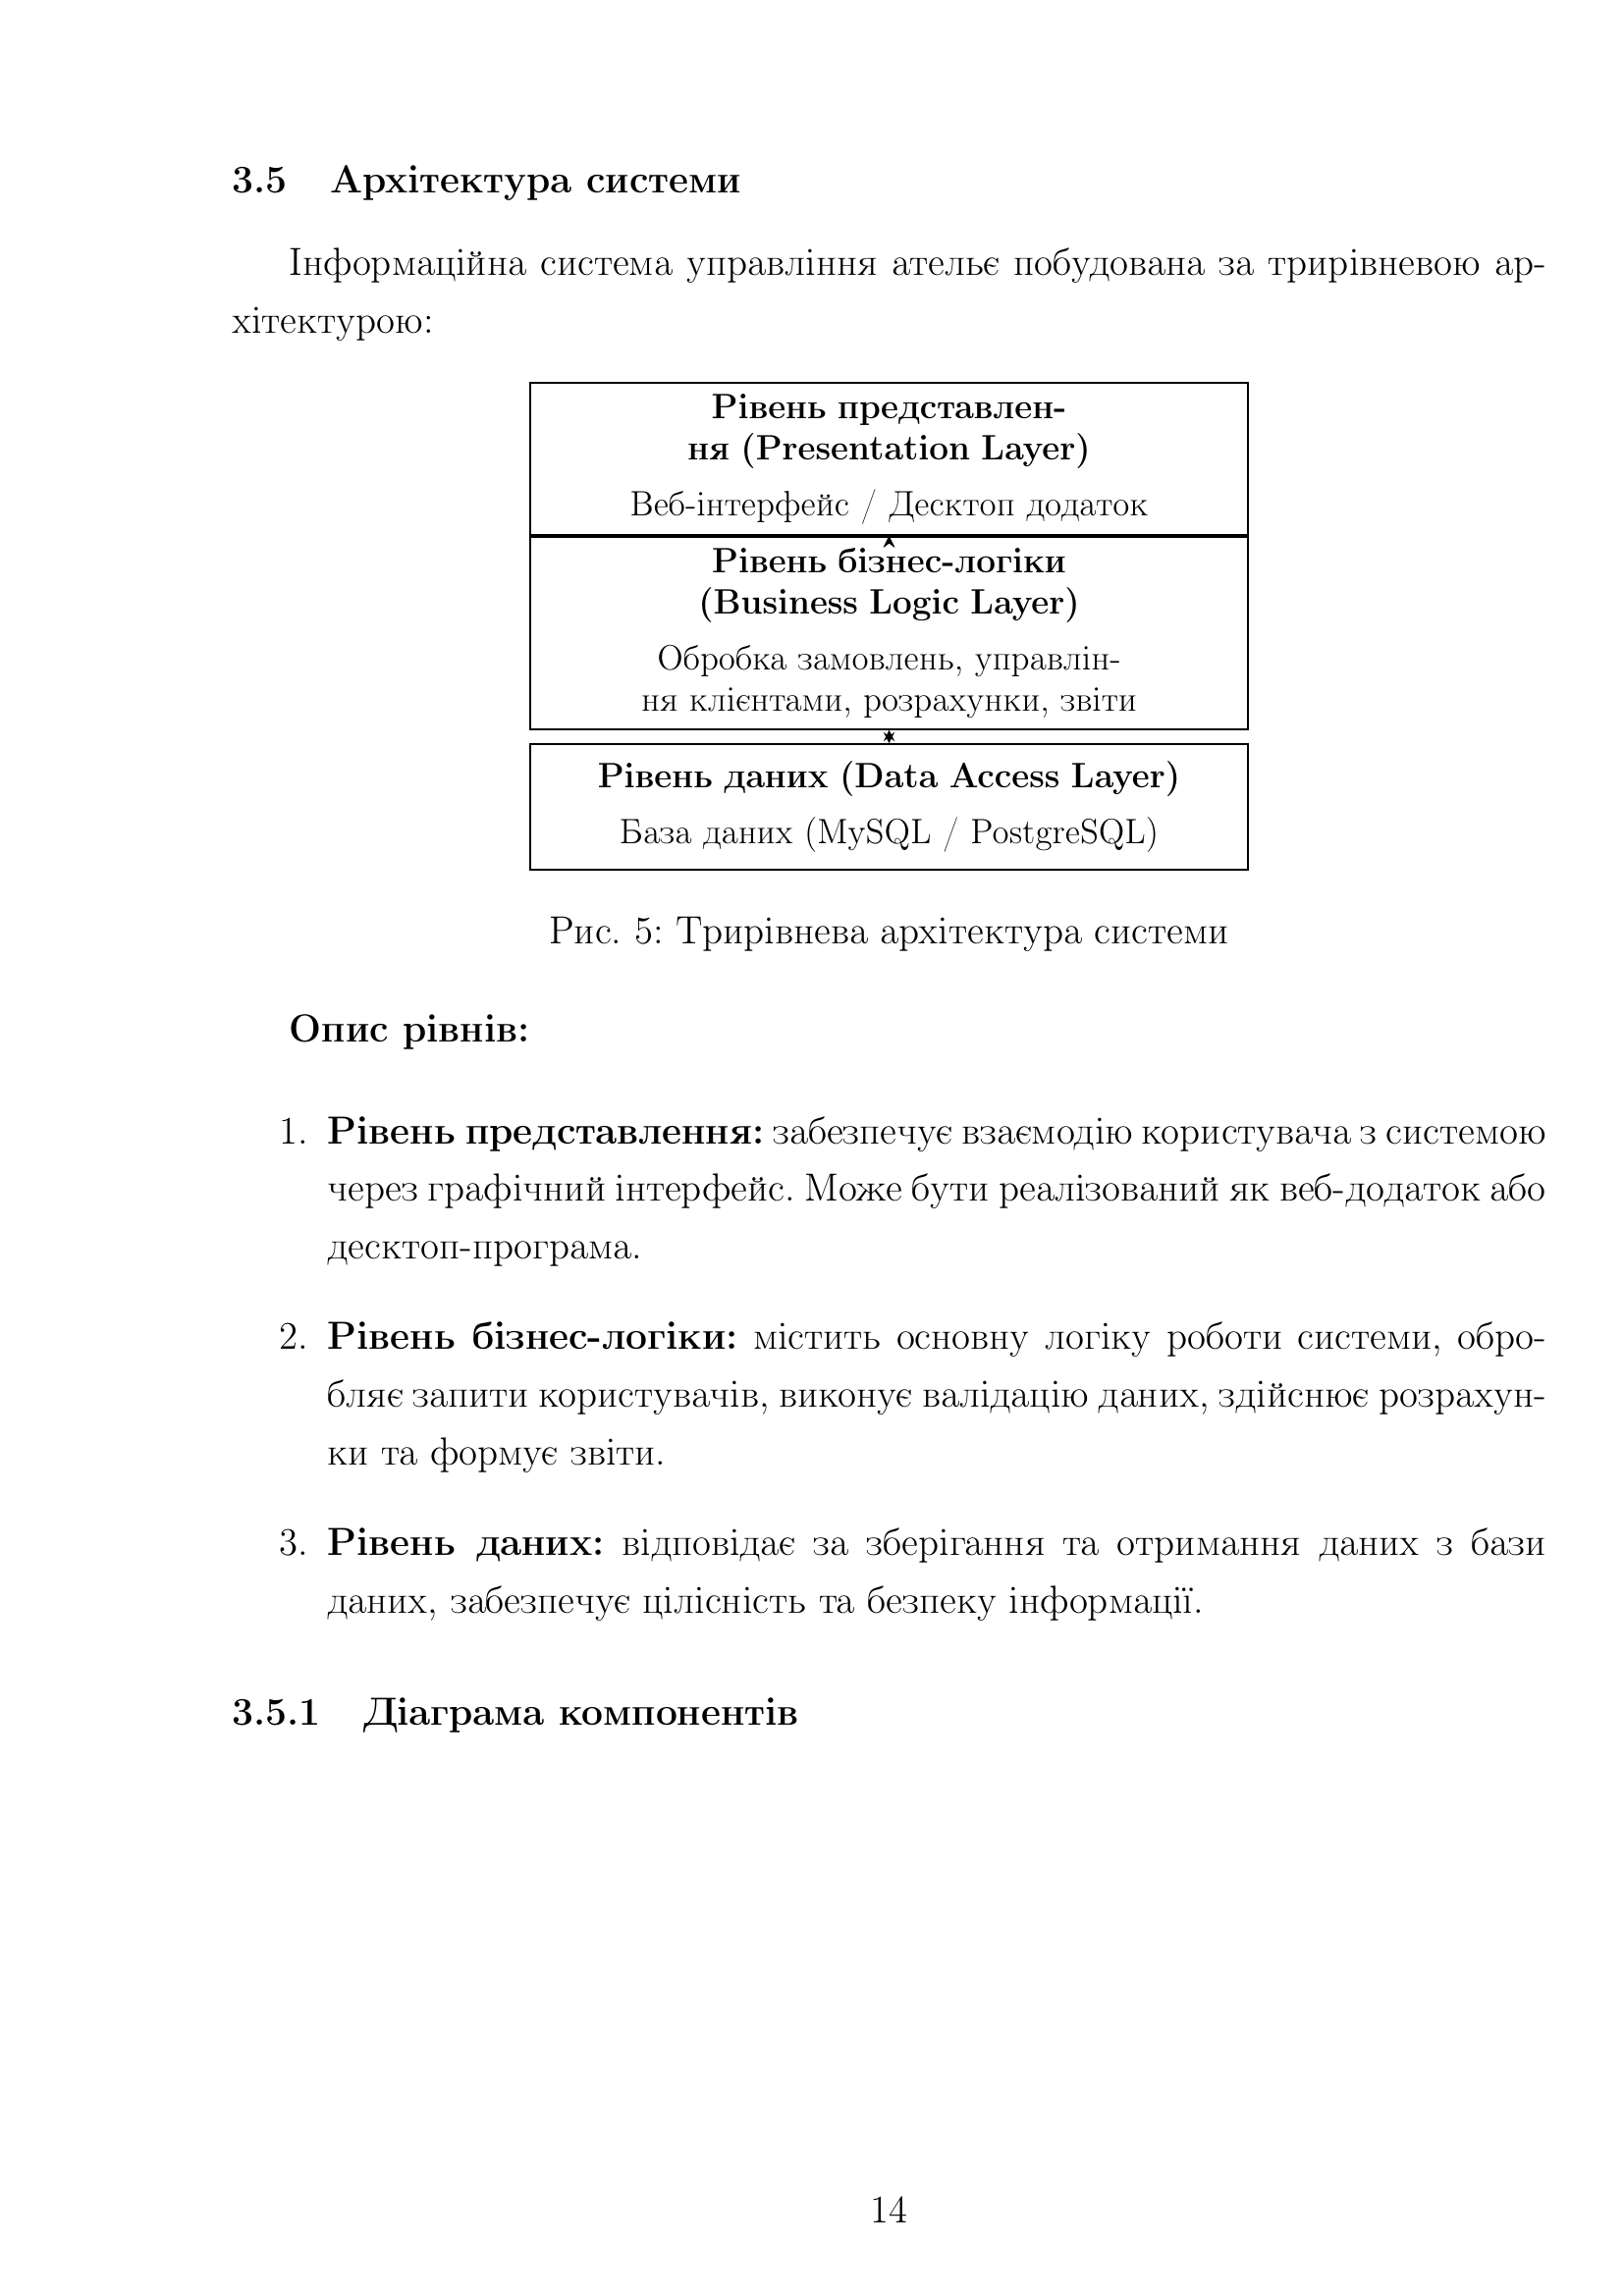
\includegraphics[width=0.85\textwidth]{diagrams/diagram-15.png}
\caption{Діаграма моніторингу та логування}
\end{figure}

\newpage

\begin{figure}[h!]
\centering
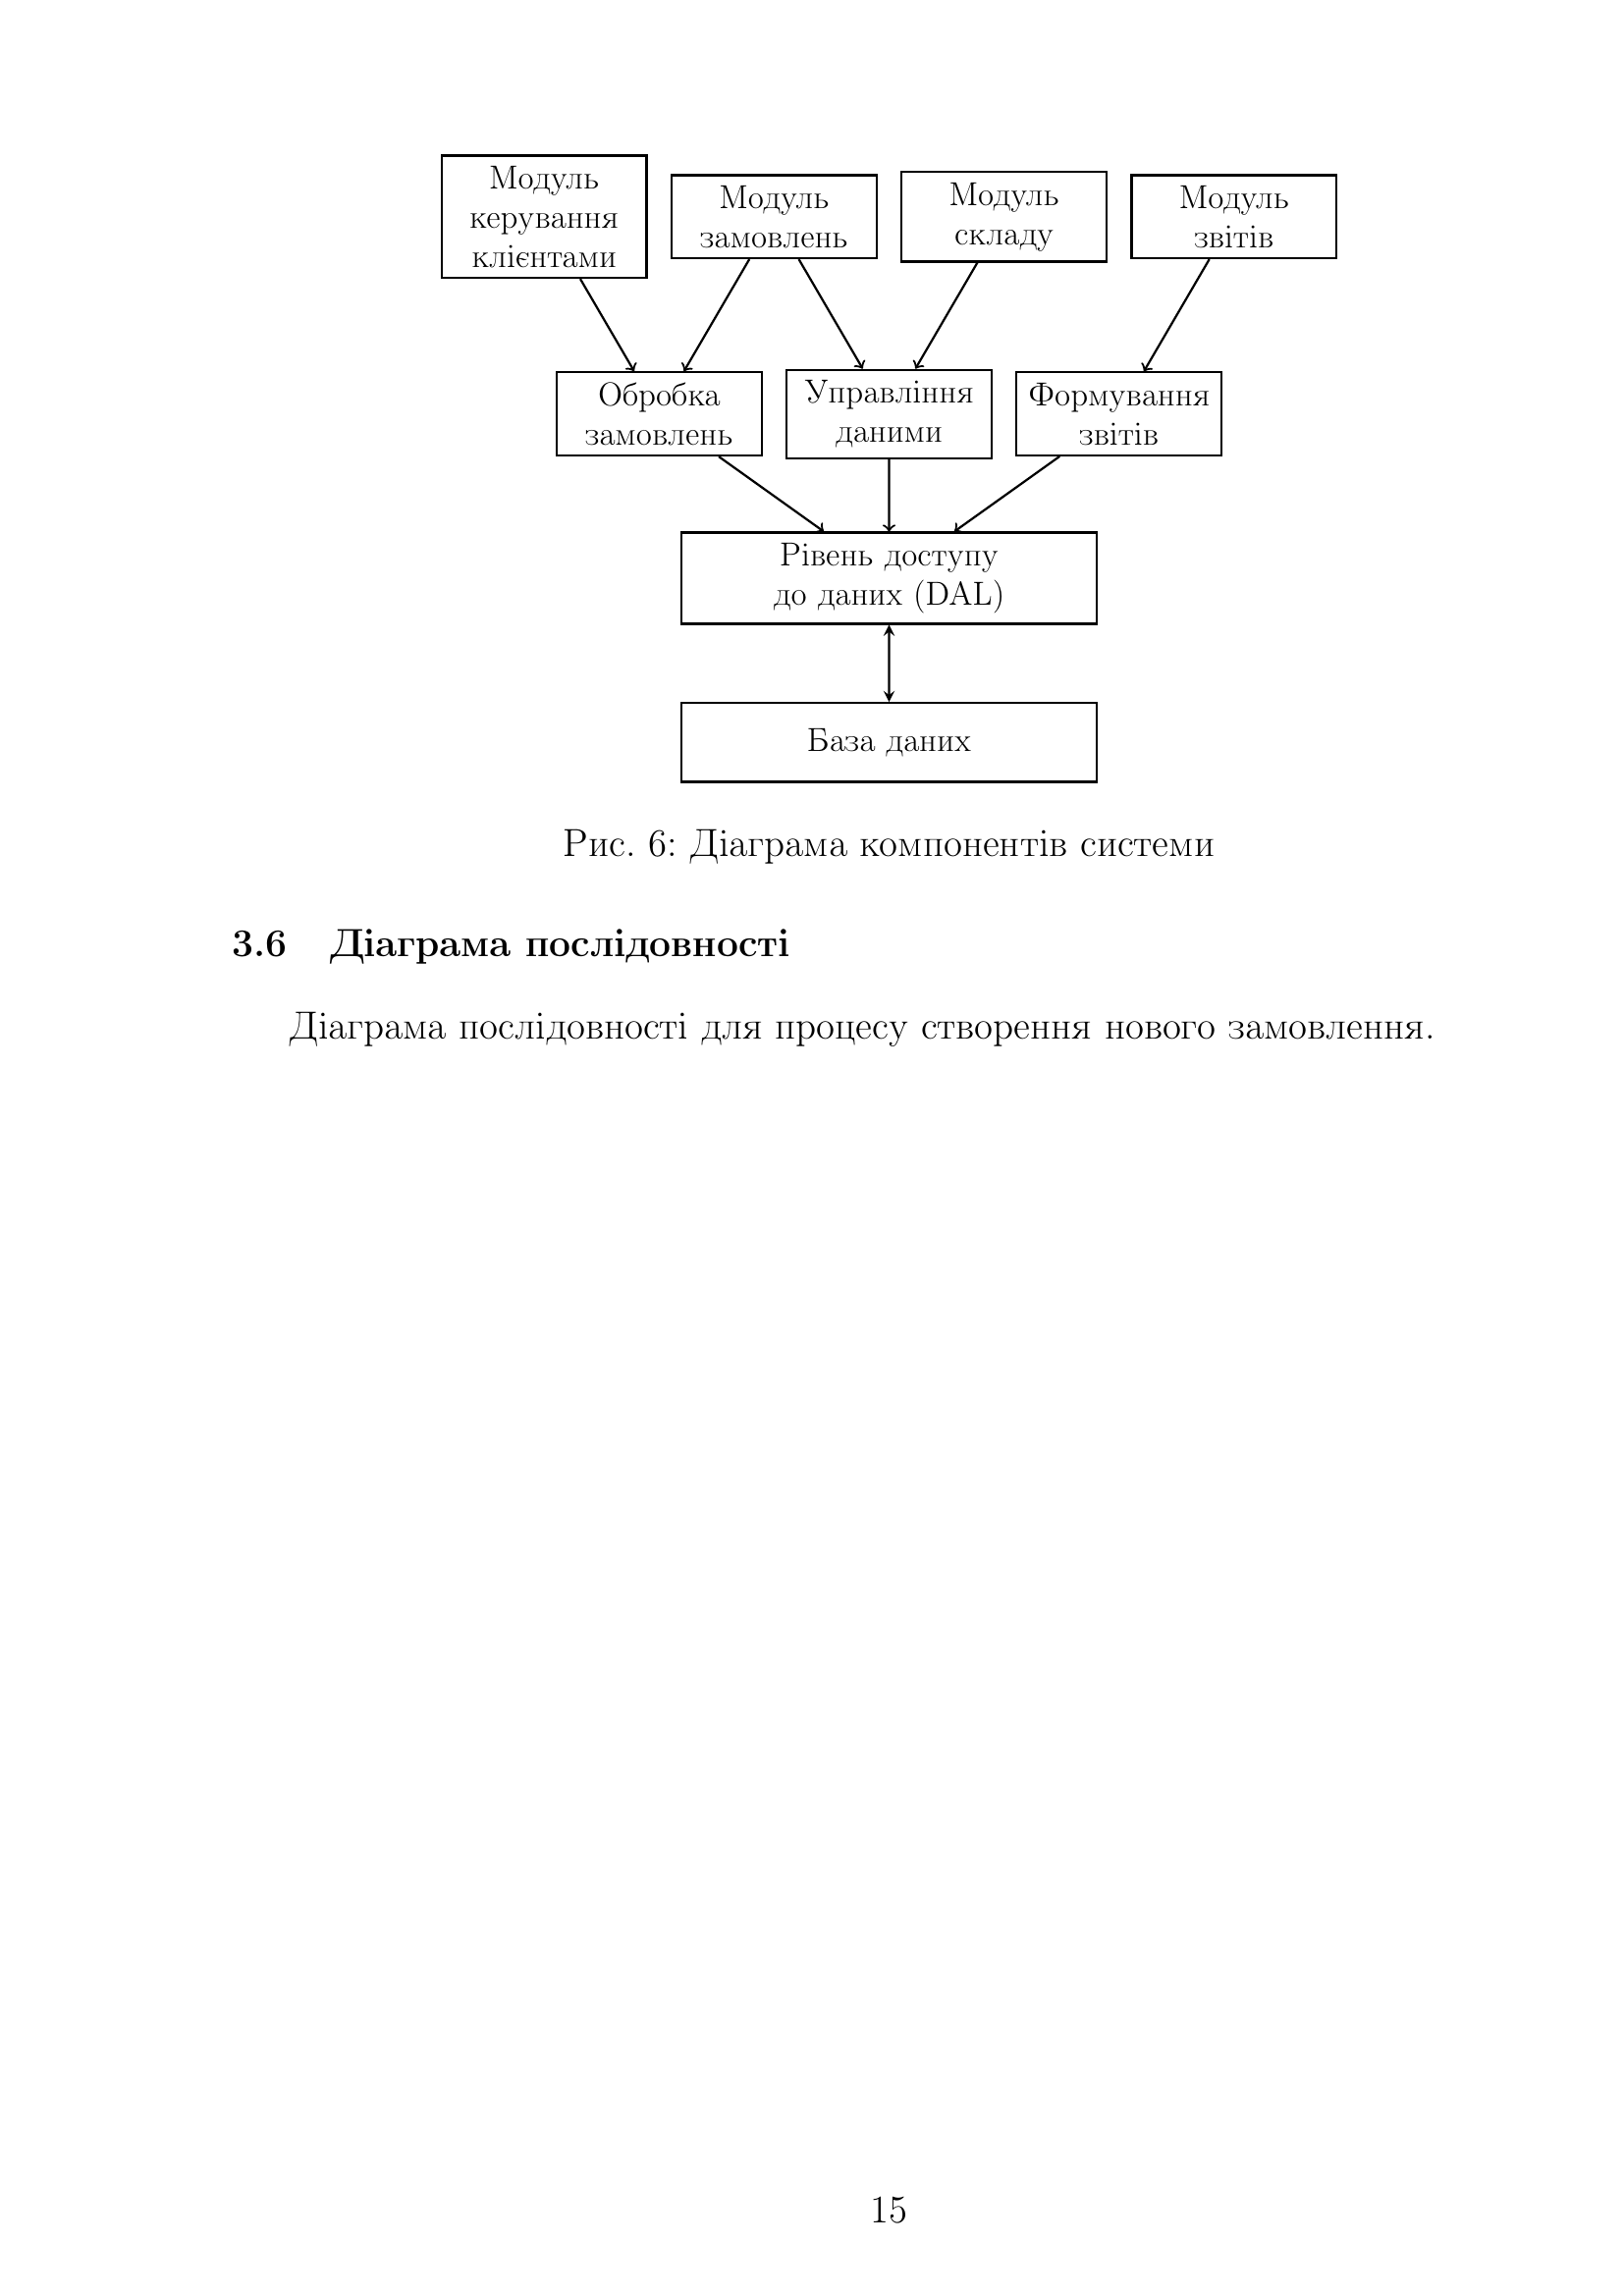
\includegraphics[width=0.85\textwidth]{diagrams/diagram-16.png}
\caption{Діаграма масштабування системи}
\end{figure}

\begin{figure}[h!]
\centering
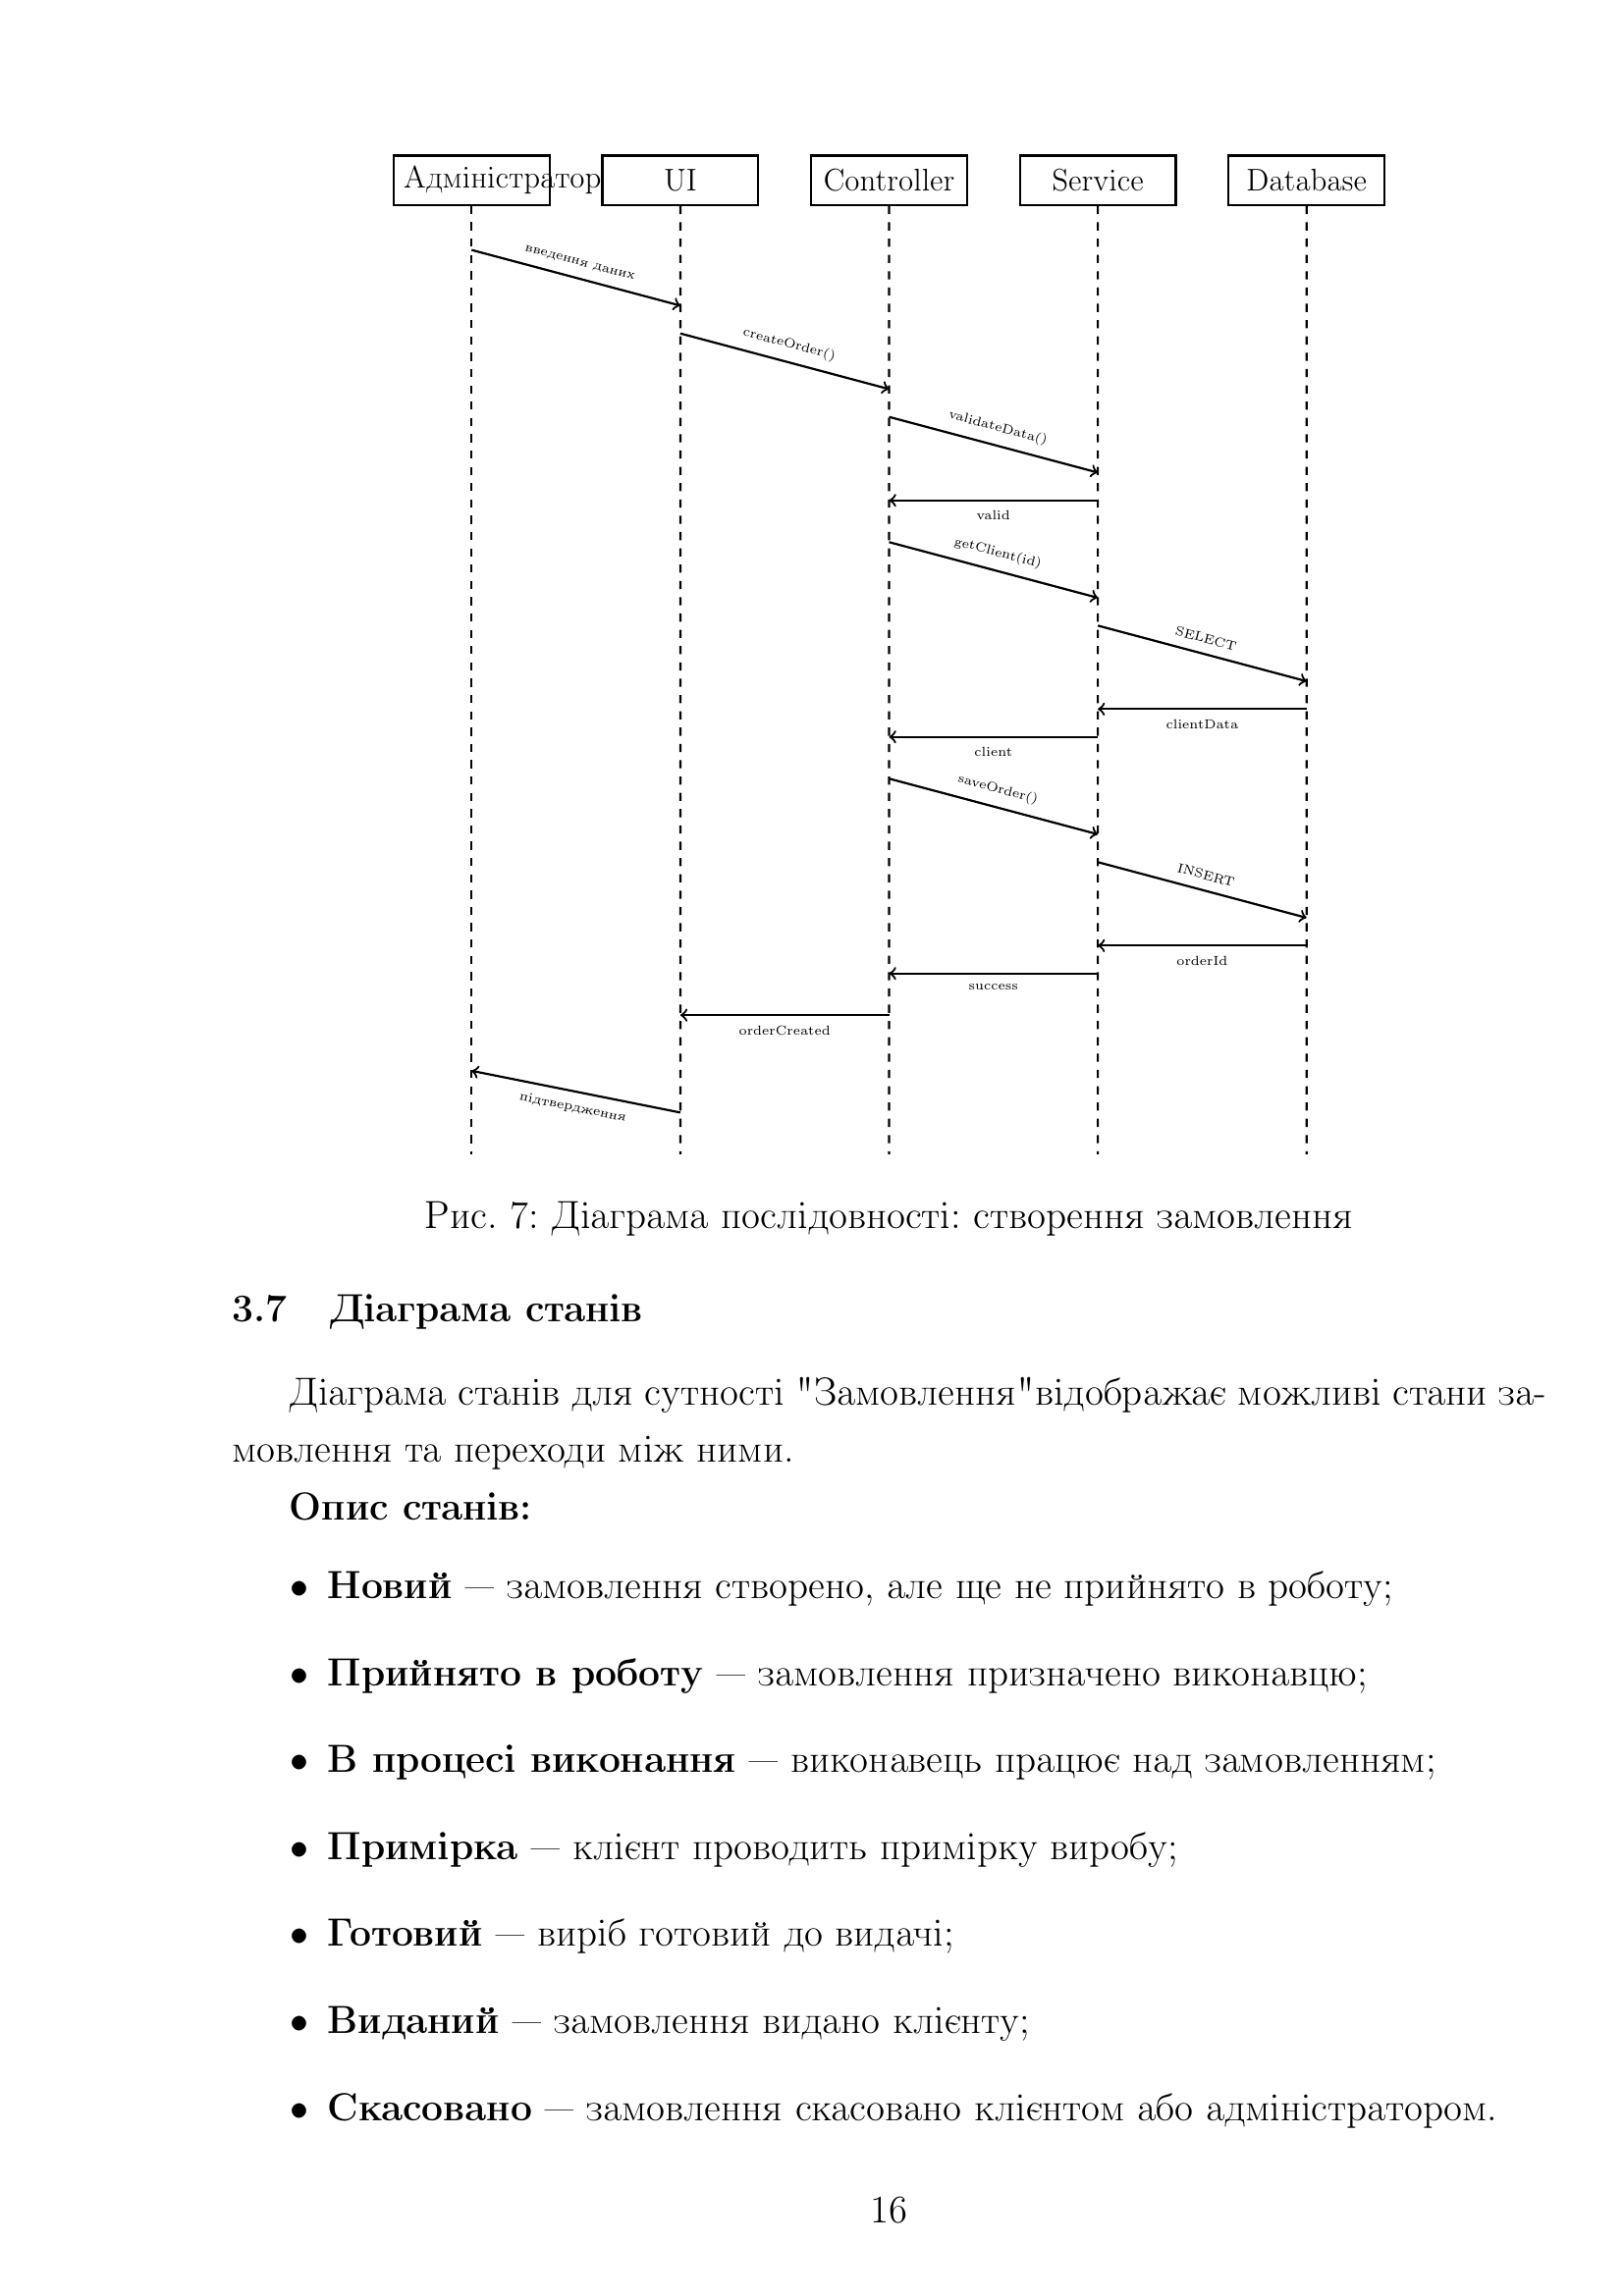
\includegraphics[width=0.85\textwidth]{diagrams/diagram-17.png}
\caption{Діаграма резервного копіювання}
\end{figure}

\newpage

\begin{figure}[h!]
\centering
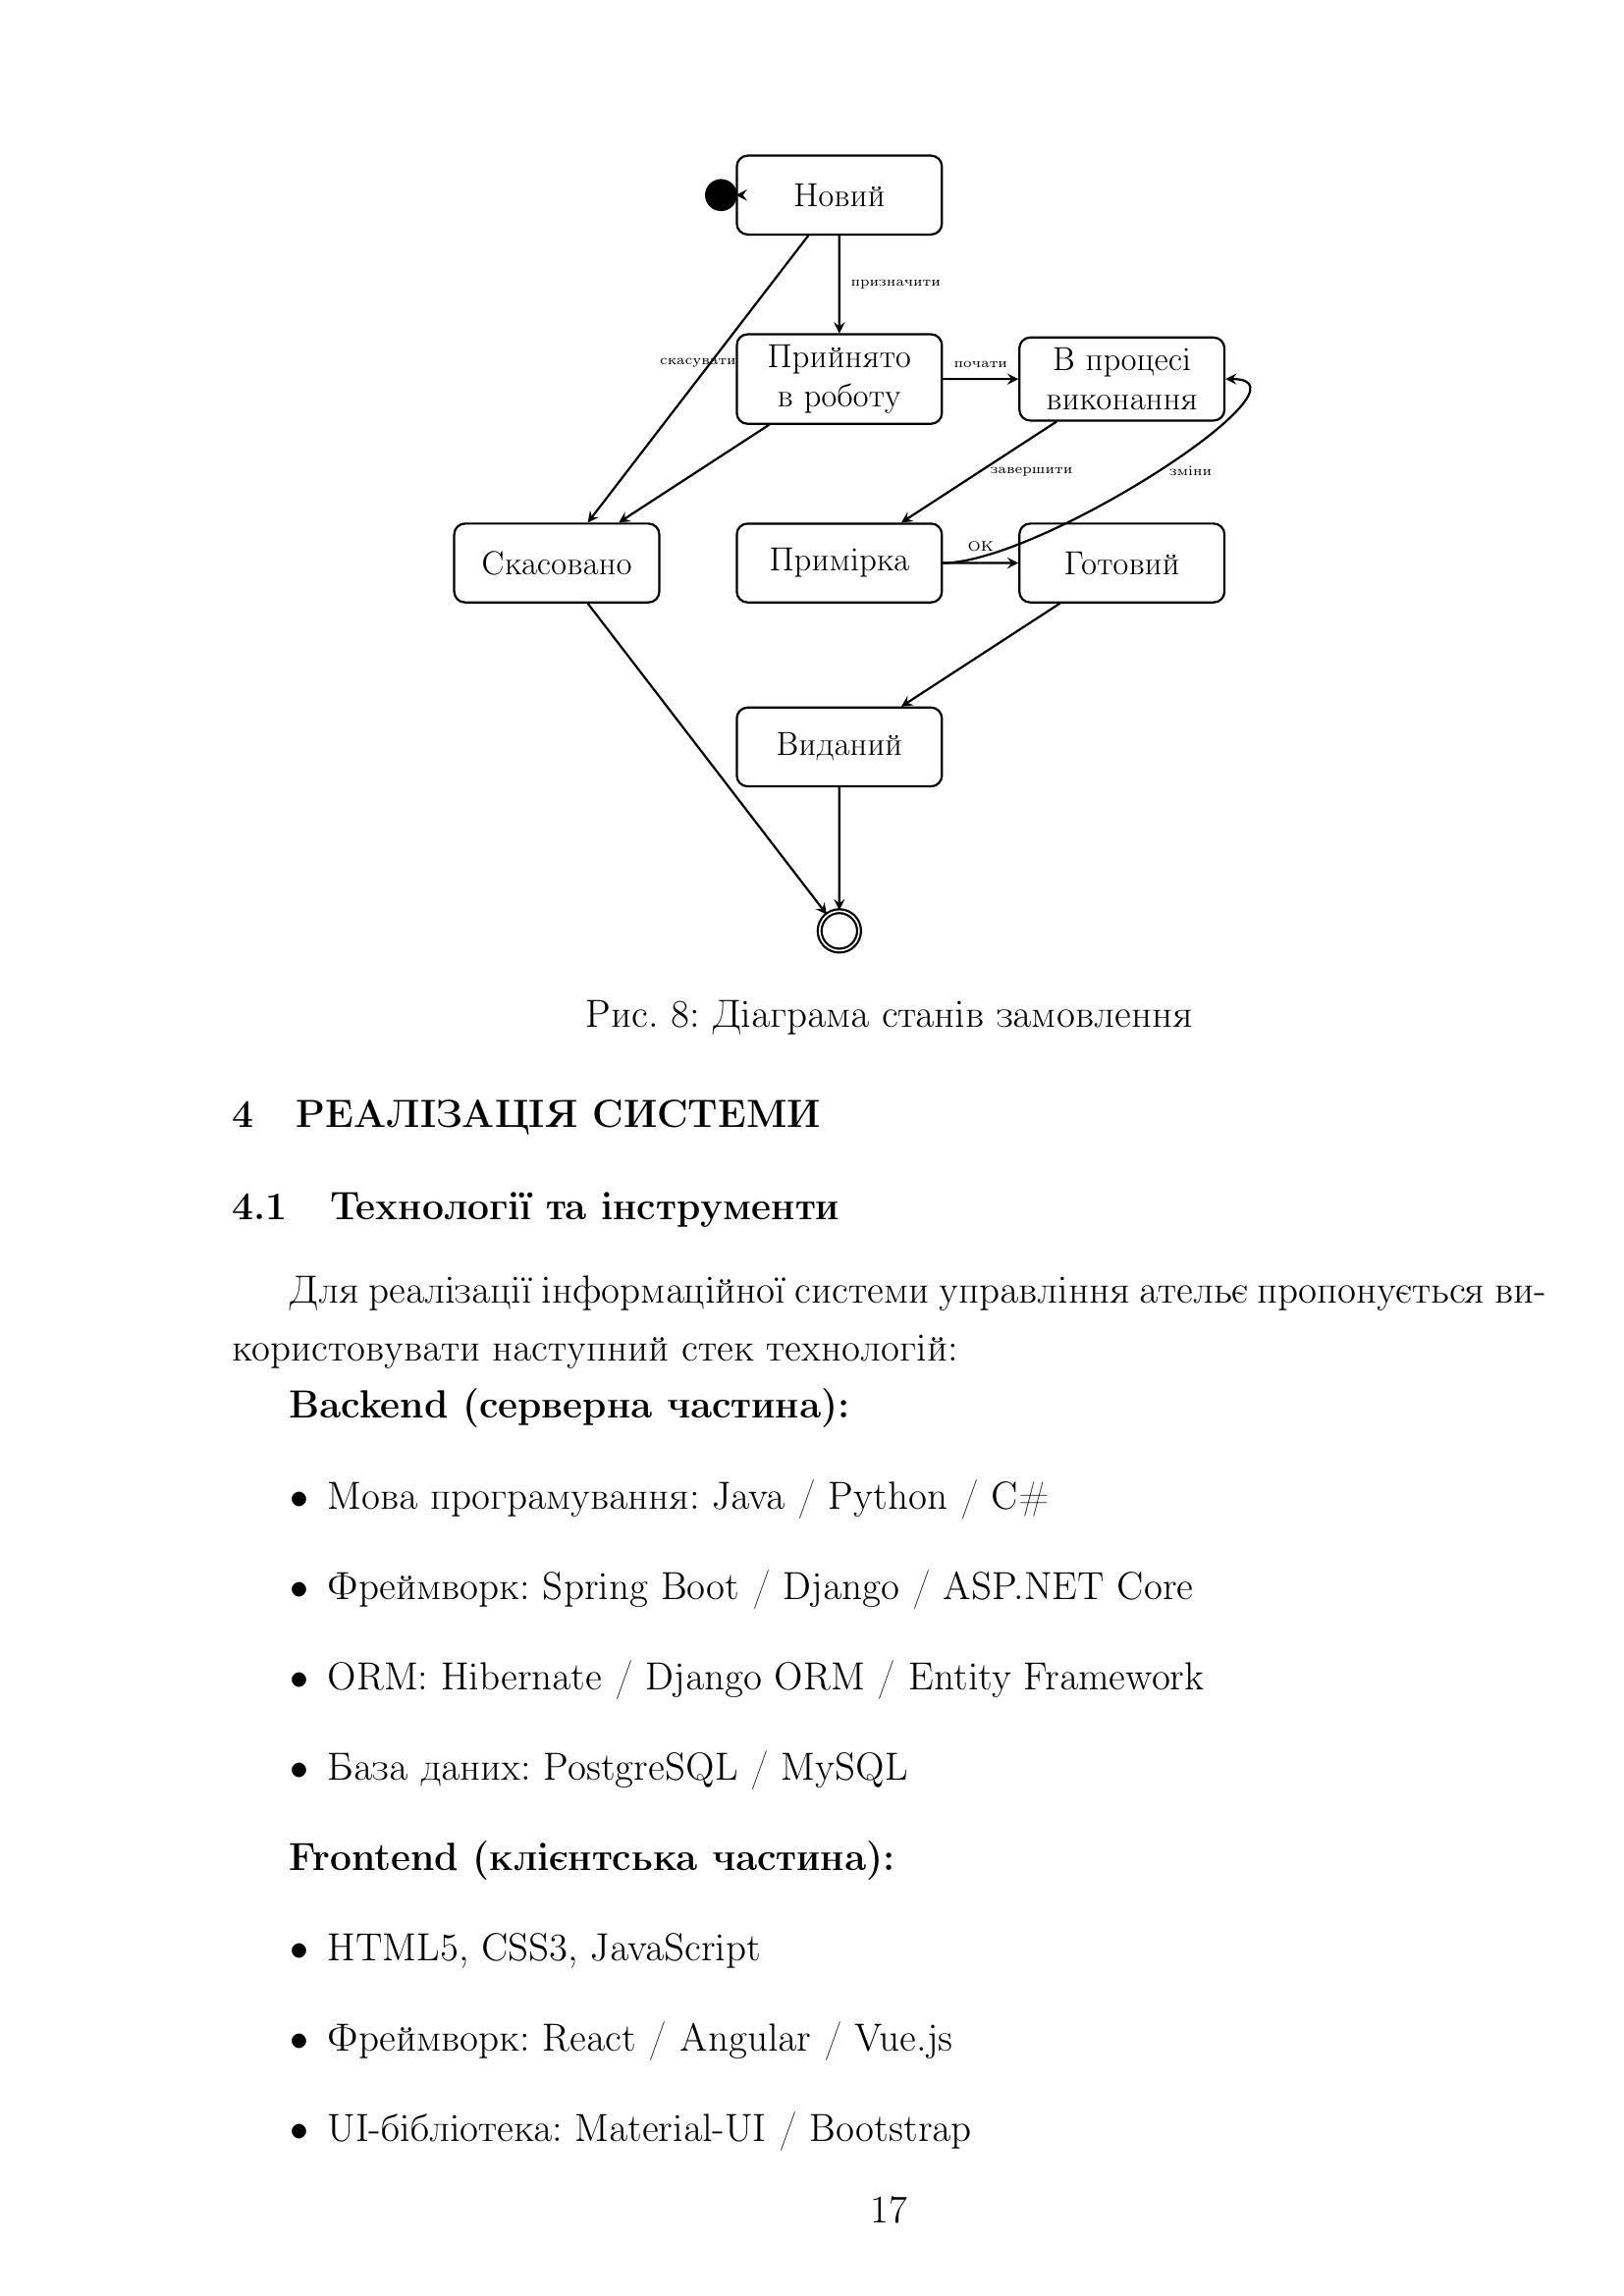
\includegraphics[width=0.85\textwidth]{diagrams/diagram-18.png}
\caption{Діаграма продуктивності системи}
\end{figure}

\newpage
\section{SQL ЗАПИТИ ТА СЕРВІСНА ЛОГІКА}

\subsection{SQL запити для роботи з базою даних}

Система використовує складні SQL запити для отримання аналітичної інформації.

\begin{lstlisting}[language=SQL, caption=Запит для звіту по виконаних замовленнях, basicstyle=\small\ttfamily, breaklines=true, frame=single]
-- Zvit po vykonanykh zamovlennyakh za period
SELECT 
    o.order_id,
    CONCAT(c.first_name, ' ', c.last_name) AS client_name,
    CONCAT(w.first_name, ' ', w.last_name) AS worker_name,
    o.order_date,
    o.completion_date,
    o.total_price,
    STRING_AGG(s.name, ', ') AS services
FROM "order" o
INNER JOIN client c ON o.client_id = c.client_id
LEFT JOIN worker w ON o.worker_id = w.worker_id
INNER JOIN order_item oi ON o.order_id = oi.order_id
INNER JOIN service s ON oi.service_id = s.service_id
WHERE o.status = 'Completed'
    AND o.completion_date BETWEEN '2025-01-01' AND '2025-12-31'
GROUP BY o.order_id, c.first_name, c.last_name, 
         w.first_name, w.last_name
ORDER BY o.completion_date DESC;
\end{lstlisting}

\begin{lstlisting}[language=SQL, caption=Запит для аналізу продуктивності працівників, basicstyle=\small\ttfamily, breaklines=true, frame=single]
-- Analiz produktyvnosti pratsivnykiv
SELECT 
    w.worker_id,
    CONCAT(w.first_name, ' ', w.last_name) AS worker_name,
    w.position,
    COUNT(o.order_id) AS total_orders,
    SUM(CASE WHEN o.status = 'Completed' THEN 1 ELSE 0 END) 
        AS completed_orders,
    SUM(CASE WHEN o.status = 'Completed' THEN o.total_price ELSE 0 END) 
        AS total_revenue,
    AVG(CASE WHEN o.status = 'Completed' 
        THEN EXTRACT(DAY FROM (o.completion_date - o.order_date)) 
        ELSE NULL END) AS avg_completion_days
FROM worker w
LEFT JOIN "order" o ON w.worker_id = o.worker_id
WHERE o.order_date >= CURRENT_DATE - INTERVAL '30 days'
GROUP BY w.worker_id, w.first_name, w.last_name, w.position
ORDER BY total_revenue DESC;
\end{lstlisting}

\newpage
\begin{lstlisting}[language=SQL, caption=Запит для контролю залишків матеріалів, basicstyle=\small\ttfamily, breaklines=true, frame=single]
-- Kontrol zalyshkiv materialiv
SELECT 
    m.material_id,
    m.name,
    m.unit,
    m.stock_quantity,
    m.min_stock_level,
    m.price_per_unit,
    CASE 
        WHEN m.stock_quantity < m.min_stock_level 
        THEN 'CRITICAL'
        WHEN m.stock_quantity < m.min_stock_level * 1.5 
        THEN 'LOW'
        ELSE 'OK'
    END AS stock_status,
    (m.min_stock_level * 2 - m.stock_quantity) 
        AS suggested_order_quantity,
    m.supplier
FROM material m
WHERE m.stock_quantity <= m.min_stock_level * 1.5
ORDER BY stock_status DESC, m.stock_quantity ASC;
\end{lstlisting}

\begin{lstlisting}[language=SQL, caption=Запит для фінансового звіту, basicstyle=\small\ttfamily, breaklines=true, frame=single]
-- Finansovyy zvit za period
WITH monthly_revenue AS (
    SELECT 
        DATE_TRUNC('month', o.completion_date) AS month,
        SUM(o.total_price) AS revenue,
        COUNT(o.order_id) AS order_count
    FROM "order" o
    WHERE o.status = 'Completed'
        AND o.completion_date >= CURRENT_DATE - INTERVAL '12 months'
    GROUP BY DATE_TRUNC('month', o.completion_date)
),
monthly_materials AS (
    SELECT 
        DATE_TRUNC('month', mu.usage_date) AS month,
        SUM(mu.cost) AS material_cost
    FROM material_usage mu
    WHERE mu.usage_date >= CURRENT_DATE - INTERVAL '12 months'
    GROUP BY DATE_TRUNC('month', mu.usage_date)
)
SELECT 
    mr.month,
    mr.order_count,
    mr.revenue,
    COALESCE(mm.material_cost, 0) AS material_cost,
    (mr.revenue - COALESCE(mm.material_cost, 0)) AS profit
FROM monthly_revenue mr
LEFT JOIN monthly_materials mm ON mr.month = mm.month
ORDER BY mr.month DESC;
\end{lstlisting}

\newpage
\subsection{Сервісний шар на C\#}

Бізнес-логіка системи реалізована у сервісному шарі з використанням принципів SOLID.

\begin{lstlisting}[language={[Sharp]C}, caption=OrderService з бізнес-логікою, basicstyle=\small\ttfamily, breaklines=true, frame=single]
namespace AtelierManagementSystem.Core.Services
{
    public class OrderService : IOrderService
    {
        private readonly IOrderRepository _orderRepository;
        private readonly IClientRepository _clientRepository;
        private readonly IMaterialRepository _materialRepository;
        private readonly ILogger<OrderService> _logger;
        
        public OrderService(
            IOrderRepository orderRepository,
            IClientRepository clientRepository,
            IMaterialRepository materialRepository,
            ILogger<OrderService> logger)
        {
            _orderRepository = orderRepository;
            _clientRepository = clientRepository;
            _materialRepository = materialRepository;
            _logger = logger;
        }
        
        public async Task<OrderDto> CreateOrderAsync(CreateOrderDto dto)
        {
            // Validate client exists
            var client = await _clientRepository.GetByIdAsync(dto.ClientId);
            if (client == null)
            {
                throw new InvalidOperationException(
                    $"Client with ID {dto.ClientId} not found");
            }
            
            // Check material availability
            foreach (var materialItem in dto.Materials)
            {
                var material = await _materialRepository
                    .GetByIdAsync(materialItem.MaterialId);
                    
                if (material == null)
                {
                    throw new InvalidOperationException(
                        $"Material {materialItem.MaterialId} not found");
                }
                
                if (material.StockQuantity < materialItem.Quantity)
                {
                    throw new InvalidOperationException(
                        $"Insufficient stock for {material.Name}");
                }
            }
            
            // Create and configure order
            var order = new Order
            {
                ClientId = dto.ClientId,
                DueDate = dto.DueDate,
                Notes = dto.Notes,
                Status = OrderStatus.New
            };
            
            // Add order items and materials
            foreach (var item in dto.OrderItems)
            {
                order.OrderItems.Add(new OrderItem
                {
                    ServiceId = item.ServiceId,
                    Quantity = item.Quantity,
                    Price = item.Price
                });
            }
            
            order.TotalPrice = order.CalculateTotalPrice();
            await _orderRepository.AddAsync(order);
            
            _logger.LogInformation(
                "Order {OrderId} created", order.OrderId);
            
            return MapToDto(order);
        }
    }
}
\end{lstlisting}

\newpage
\section{ТЕСТУВАННЯ ТА ВПРОВАДЖЕННЯ}

\subsection{Plan тестування}

Тестування інформаційної системи включає наступні етапи:

\begin{enumerate}
    \item \textbf{Модульне тестування (Unit Testing):}
    \begin{itemize}
        \item Тестування окремих методів та функцій
        \item Перевірка коректності обчислень
        \item Валідація вхідних даних
    \end{itemize}
    
    \item \textbf{Інтеграційне тестування:}
    \begin{itemize}
        \item Тестування взаємодії між модулями
        \item Перевірка роботи з базою даних
        \item Тестування API endpoints
    \end{itemize}
    
    \item \textbf{Системне тестування:}
    \begin{itemize}
        \item Тестування повного функціоналу системи
        \item Перевірка бізнес-процесів
        \item Тестування продуктивності
    \end{itemize}
    
    \item \textbf{Приймальне тестування:}
    \begin{itemize}
        \item Тестування користувачами
        \item Перевірка відповідності вимогам
        \item Виявлення зауважень
    \end{itemize}
\end{enumerate}

\subsection{Приклади тестових сценаріїв}

\textbf{Тестовий сценарій 1: Створення нового замовлення}

\begin{enumerate}
    \item Адміністратор входить в систему
    \item Вибирає клієнта зі списку або створює нового
    \item Додає послуги до замовлення
    \item Вказує необхідні матеріали
    \item Система розраховує загальну вартість
    \item Адміністратор вказує термін виконання
    \item Система зберігає замовлення
    \item Очікуваний результат: замовлення створено, статус "Новий"
\end{enumerate}

\textbf{Тестовий сценарій 2: Відстеження виконання замовлення}

\begin{enumerate}
    \item Кравець входить в систему
    \item Переглядає список своїх замовлень
    \item Вибирає замовлення в роботі
    \item Оновлює статус на "В процесі виконання"
    \item Після завершення змінює статус на "Готовий"
    \item Очікуваний результат: статус оновлено, клієнт може бути повідомлений
\end{enumerate}

\newpage
\subsection{Модульне тестування на C\#}

Для тестування використовуються фреймворки xUnit та Moq.

\begin{lstlisting}[language={[Sharp]C}, caption=Тести для OrderService, basicstyle=\small\ttfamily, breaklines=true, frame=single]
using Xunit;
using Moq;
using FluentAssertions;

namespace AtelierManagementSystem.UnitTests.Services
{
    public class OrderServiceTests
    {
        private readonly Mock<IOrderRepository> _orderRepositoryMock;
        private readonly Mock<IClientRepository> _clientRepositoryMock;
        private readonly Mock<IMaterialRepository> _materialRepositoryMock;
        private readonly Mock<ILogger<OrderService>> _loggerMock;
        private readonly OrderService _sut;
        
        public OrderServiceTests()
        {
            _orderRepositoryMock = new Mock<IOrderRepository>();
            _clientRepositoryMock = new Mock<IClientRepository>();
            _materialRepositoryMock = new Mock<IMaterialRepository>();
            _loggerMock = new Mock<ILogger<OrderService>>();
            
            _sut = new OrderService(
                _orderRepositoryMock.Object,
                _clientRepositoryMock.Object,
                _materialRepositoryMock.Object,
                _loggerMock.Object);
        }
        
        [Fact]
        public async Task CreateOrderAsync_WithValidData_ShouldCreateOrder()
        {
            // Arrange
            var createDto = new CreateOrderDto
            {
                ClientId = 1,
                DueDate = DateTime.Now.AddDays(7),
                OrderItems = new List<CreateOrderItemDto>
                {
                    new() { ServiceId = 1, Quantity = 1, Price = 100 }
                },
                Materials = new List<CreateMaterialUsageDto>()
            };
            
            var client = new Client 
            { 
                ClientId = 1, 
                FirstName = "Ivan", 
                LastName = "Petrov" 
            };
            
            _clientRepositoryMock
                .Setup(r => r.GetByIdAsync(1))
                .ReturnsAsync(client);
            
            // Act
            var result = await _sut.CreateOrderAsync(createDto);
            
            // Assert
            result.Should().NotBeNull();
            result.ClientId.Should().Be(1);
            _orderRepositoryMock.Verify(
                r => r.AddAsync(It.IsAny<Order>()), 
                Times.Once);
        }
        
        [Fact]
        public async Task CreateOrderAsync_WithInvalidClient_ShouldThrowException()
        {
            // Arrange
            var createDto = new CreateOrderDto { ClientId = 999 };
            
            _clientRepositoryMock
                .Setup(r => r.GetByIdAsync(999))
                .ReturnsAsync((Client)null);
            
            // Act & Assert
            await Assert.ThrowsAsync<InvalidOperationException>(
                () => _sut.CreateOrderAsync(createDto));
        }
        
        [Fact]
        public async Task UpdateOrderStatus_ShouldUpdateStatus()
        {
            // Arrange
            var order = new Order 
            { 
                OrderId = 1, 
                Status = OrderStatus.New 
            };
            
            _orderRepositoryMock
                .Setup(r => r.GetByIdAsync(1))
                .ReturnsAsync(order);
            
            // Act
            await _sut.UpdateOrderStatusAsync(1, OrderStatus.InProgress);
            
            // Assert
            order.Status.Should().Be(OrderStatus.InProgress);
            _orderRepositoryMock.Verify(
                r => r.UpdateAsync(order), 
                Times.Once);
        }
    }
}
\end{lstlisting}

\newpage
\subsection{Інтеграційне тестування}

\begin{lstlisting}[language={[Sharp]C}, caption=Інтеграційні тести з базою даних, basicstyle=\small\ttfamily, breaklines=true, frame=single]
using Microsoft.EntityFrameworkCore;
using Xunit;

namespace AtelierManagementSystem.IntegrationTests
{
    public class OrderRepositoryIntegrationTests : IDisposable
    {
        private readonly AtelierDbContext _context;
        private readonly OrderRepository _repository;
        
        public OrderRepositoryIntegrationTests()
        {
            var options = new DbContextOptionsBuilder<AtelierDbContext>()
                .UseInMemoryDatabase(databaseName: "TestDb")
                .Options;
                
            _context = new AtelierDbContext(options);
            _repository = new OrderRepository(_context);
            
            SeedData();
        }
        
        private void SeedData()
        {
            var client = new Client
            {
                ClientId = 1,
                FirstName = "Test",
                LastName = "Client",
                Phone = "123456789"
            };
            
            var worker = new Worker
            {
                WorkerId = 1,
                FirstName = "Test",
                LastName = "Worker",
                Position = "Tailor"
            };
            
            var order = new Order
            {
                OrderId = 1,
                ClientId = 1,
                WorkerId = 1,
                OrderDate = DateTime.Now,
                DueDate = DateTime.Now.AddDays(5),
                Status = OrderStatus.New,
                TotalPrice = 500
            };
            
            _context.Clients.Add(client);
            _context.Workers.Add(worker);
            _context.Orders.Add(order);
            _context.SaveChanges();
        }
        
        [Fact]
        public async Task GetByIdAsync_ShouldReturnOrderWithRelations()
        {
            // Act
            var result = await _repository.GetByIdAsync(1);
            
            // Assert
            Assert.NotNull(result);
            Assert.Equal(1, result.OrderId);
            Assert.NotNull(result.Client);
            Assert.Equal("Test", result.Client.FirstName);
            Assert.NotNull(result.Worker);
        }
        
        [Fact]
        public async Task GetOrdersByStatusAsync_ShouldReturnFilteredOrders()
        {
            // Act
            var results = await _repository
                .GetOrdersByStatusAsync(OrderStatus.New);
            
            // Assert
            Assert.NotEmpty(results);
            Assert.All(results, o => 
                Assert.Equal(OrderStatus.New, o.Status));
        }
        
        public void Dispose()
        {
            _context.Database.EnsureDeleted();
            _context.Dispose();
        }
    }
}
\end{lstlisting}

\newpage
\subsection{Конфігурація та Dependency Injection}

\begin{lstlisting}[language={[Sharp]C}, caption=Конфігурація сервісів у Program.cs, basicstyle=\small\ttfamily, breaklines=true, frame=single]
using Microsoft.EntityFrameworkCore;
using AtelierManagementSystem.Infrastructure.Data;

var builder = WebApplication.CreateBuilder(args);

// Add services to the container
builder.Services.AddControllers();
builder.Services.AddEndpointsApiExplorer();
builder.Services.AddSwaggerGen();

// Database configuration
builder.Services.AddDbContext<AtelierDbContext>(options =>
    options.UseSqlServer(
        builder.Configuration.GetConnectionString("DefaultConnection"),
        b => b.MigrationsAssembly("AtelierManagementSystem.Infrastructure")
    ));

// Register repositories
builder.Services.AddScoped<IOrderRepository, OrderRepository>();
builder.Services.AddScoped<IClientRepository, ClientRepository>();
builder.Services.AddScoped<IWorkerRepository, WorkerRepository>();
builder.Services.AddScoped<IMaterialRepository, MaterialRepository>();
builder.Services.AddScoped<IServiceRepository, ServiceRepository>();

// Register services
builder.Services.AddScoped<IOrderService, OrderService>();
builder.Services.AddScoped<IClientService, ClientService>();
builder.Services.AddScoped<IReportService, ReportService>();

// Add CORS
builder.Services.AddCors(options =>
{
    options.AddPolicy("AllowAll",
        policy => policy
            .AllowAnyOrigin()
            .AllowAnyMethod()
            .AllowAnyHeader());
});

// Add logging
builder.Services.AddLogging(config =>
{
    config.AddConsole();
    config.AddDebug();
});

var app = builder.Build();

// Configure the HTTP request pipeline
if (app.Environment.IsDevelopment())
{
    app.UseSwagger();
    app.UseSwaggerUI();
}

app.UseHttpsRedirection();
app.UseCors("AllowAll");
app.UseAuthorization();
app.MapControllers();

app.Run();
\end{lstlisting}

\newpage
\subsection{Конфігурація підключення до бази даних}

\begin{lstlisting}[language=JavaScript, caption=appsettings.json, basicstyle=\small\ttfamily, breaklines=true, frame=single]
{
  "ConnectionStrings": {
    "DefaultConnection": "Server=localhost;Database=AtelierDB;
      User Id=sa;Password=YourPassword;TrustServerCertificate=True"
  },
  "Logging": {
    "LogLevel": {
      "Default": "Information",
      "Microsoft.AspNetCore": "Warning",
      "Microsoft.EntityFrameworkCore": "Information"
    }
  },
  "AllowedHosts": "*",
  "Jwt": {
    "Key": "YourSecretKeyForJWTAuthentication",
    "Issuer": "AtelierManagementSystem",
    "Audience": "AtelierUsers",
    "ExpiryInMinutes": 60
  },
  "EmailSettings": {
    "SmtpServer": "smtp.gmail.com",
    "SmtpPort": 587,
    "FromEmail": "noreply@atelier.com",
    "FromName": "Atelier Management System"
  }
}
\end{lstlisting}

\subsection{Міграції бази даних}

Entity Framework Core використовує міграції для управління схемою бази даних.

\begin{lstlisting}[language={[Sharp]C}, caption=Початкова міграція, basicstyle=\small\ttfamily, breaklines=true, frame=single]
using Microsoft.EntityFrameworkCore.Migrations;

public partial class InitialCreate : Migration
{
    protected override void Up(MigrationBuilder migrationBuilder)
    {
        migrationBuilder.CreateTable(
            name: "Clients",
            columns: table => new
            {
                ClientId = table.Column<int>(nullable: false)
                    .Annotation("SqlServer:Identity", "1, 1"),
                FirstName = table.Column<string>(maxLength: 50, nullable: false),
                LastName = table.Column<string>(maxLength: 50, nullable: false),
                Phone = table.Column<string>(maxLength: 20, nullable: true),
                Email = table.Column<string>(maxLength: 100, nullable: true),
                RegistrationDate = table.Column<DateTime>(nullable: false),
                Notes = table.Column<string>(nullable: true)
            },
            constraints: table =>
            {
                table.PrimaryKey("PK_Clients", x => x.ClientId);
            });
            
        migrationBuilder.CreateIndex(
            name: "IX_Clients_Phone",
            table: "Clients",
            column: "Phone");
    }
    
    protected override void Down(MigrationBuilder migrationBuilder)
    {
        migrationBuilder.DropTable(name: "Clients");
    }
}
\end{lstlisting}

\textbf{Команди для роботи з міграціями:}

\begin{verbatim}
# Створення нової міграції
dotnet ef migrations add InitialCreate --project Infrastructure

# Застосування міграцій до бази даних
dotnet ef database update --project Infrastructure

# Відкат останньої міграції
dotnet ef migrations remove --project Infrastructure

# Створення SQL скрипту з міграцій
dotnet ef migrations script --project Infrastructure
\end{verbatim}

\newpage
\subsection{Безпека та автентифікація}

\begin{lstlisting}[language={[Sharp]C}, caption=JWT автентифікація, basicstyle=\small\ttfamily, breaklines=true, frame=single]
using Microsoft.AspNetCore.Authentication.JwtBearer;
using Microsoft.IdentityModel.Tokens;
using System.Text;

// У Program.cs додати:
builder.Services.AddAuthentication(JwtBearerDefaults.AuthenticationScheme)
    .AddJwtBearer(options =>
    {
        options.TokenValidationParameters = new TokenValidationParameters
        {
            ValidateIssuer = true,
            ValidateAudience = true,
            ValidateLifetime = true,
            ValidateIssuerSigningKey = true,
            ValidIssuer = builder.Configuration["Jwt:Issuer"],
            ValidAudience = builder.Configuration["Jwt:Audience"],
            IssuerSigningKey = new SymmetricSecurityKey(
                Encoding.UTF8.GetBytes(builder.Configuration["Jwt:Key"]))
        };
    });

builder.Services.AddAuthorization(options =>
{
    options.AddPolicy("AdminOnly", policy => 
        policy.RequireRole("Administrator"));
    options.AddPolicy("WorkerOrAdmin", policy => 
        policy.RequireRole("Administrator", "Worker"));
});
\end{lstlisting}

\begin{lstlisting}[language={[Sharp]C}, caption=Сервіс генерації JWT токенів, basicstyle=\small\ttfamily, breaklines=true, frame=single]
using System.IdentityModel.Tokens.Jwt;
using System.Security.Claims;
using Microsoft.IdentityModel.Tokens;

public class JwtTokenService
{
    private readonly IConfiguration _configuration;
    
    public JwtTokenService(IConfiguration configuration)
    {
        _configuration = configuration;
    }
    
    public string GenerateToken(User user)
    {
        var claims = new List<Claim>
        {
            new Claim(ClaimTypes.NameIdentifier, user.Id.ToString()),
            new Claim(ClaimTypes.Name, user.Username),
            new Claim(ClaimTypes.Email, user.Email),
            new Claim(ClaimTypes.Role, user.Role)
        };
        
        var key = new SymmetricSecurityKey(
            Encoding.UTF8.GetBytes(_configuration["Jwt:Key"]));
        var credentials = new SigningCredentials(
            key, SecurityAlgorithms.HmacSha256);
        
        var token = new JwtSecurityToken(
            issuer: _configuration["Jwt:Issuer"],
            audience: _configuration["Jwt:Audience"],
            claims: claims,
            expires: DateTime.Now.AddMinutes(
                Convert.ToDouble(_configuration["Jwt:ExpiryInMinutes"])),
            signingCredentials: credentials
        );
        
        return new JwtSecurityTokenHandler().WriteToken(token);
    }
}
\end{lstlisting}

\newpage
\subsection{Впровадження системи}

Етапи впровадження:

\begin{enumerate}
    \item \textbf{Підготовчий етап:}
    \begin{itemize}
        \item Налаштування серверного обладнання
        \item Встановлення програмного забезпечення
        \item Створення бази даних
    \end{itemize}
    
    \item \textbf{Міграція даних:}
    \begin{itemize}
        \item Перенесення існуючих даних про клієнтів
        \item Імпорт каталогу послуг
        \item Завантаження довідників
    \end{itemize}
    
    \item \textbf{Навчання персоналу:}
    \begin{itemize}
        \item Проведення тренінгів для адміністраторів
        \item Навчання кравців роботі з системою
        \item Підготовка інструкцій користувача
    \end{itemize}
    
    \item \textbf{Пілотний запуск:}
    \begin{itemize}
        \item Робота в тестовому режимі
        \item Виявлення та усунення помилок
        \item Збір зворотного зв'язку
    \end{itemize}
    
    \item \textbf{Промислова експлуатація:}
    \begin{itemize}
        \item Повний перехід на нову систему
        \item Технічна підтримка
        \item Моніторинг роботи системи
    \end{itemize}
\end{enumerate}

\newpage
\section{ЗВІТНІСТЬ ТА МОНІТОРИНГ}

\subsection{Система звітів}

\begin{lstlisting}[language={[Sharp]C}, caption=Сервіс формування звітів, basicstyle=\small\ttfamily, breaklines=true, frame=single]
namespace AtelierManagementSystem.Core.Services
{
    public class ReportService : IReportService
    {
        private readonly AtelierDbContext _context;
        
        public async Task<FinancialReportDto> GenerateFinancialReportAsync(
            DateTime startDate, DateTime endDate)
        {
            var orders = await _context.Orders
                .Include(o => o.MaterialUsages)
                .Where(o => o.Status == OrderStatus.Completed &&
                           o.CompletionDate >= startDate &&
                           o.CompletionDate <= endDate)
                .ToListAsync();
            
            var totalRevenue = orders.Sum(o => o.TotalPrice);
            var totalMaterialCost = orders
                .SelectMany(o => o.MaterialUsages)
                .Sum(m => m.Cost);
            
            var ordersByMonth = orders
                .GroupBy(o => new { 
                    o.CompletionDate.Value.Year, 
                    o.CompletionDate.Value.Month 
                })
                .Select(g => new MonthlyStats
                {
                    Year = g.Key.Year,
                    Month = g.Key.Month,
                    OrderCount = g.Count(),
                    Revenue = g.Sum(o => o.TotalPrice),
                    MaterialCost = g.SelectMany(o => o.MaterialUsages)
                        .Sum(m => m.Cost)
                })
                .OrderBy(m => m.Year).ThenBy(m => m.Month)
                .ToList();
            
            return new FinancialReportDto
            {
                StartDate = startDate,
                EndDate = endDate,
                TotalOrders = orders.Count,
                TotalRevenue = totalRevenue,
                TotalMaterialCost = totalMaterialCost,
                NetProfit = totalRevenue - totalMaterialCost,
                MonthlyBreakdown = ordersByMonth
            };
        }
        
        public async Task<WorkerPerformanceReportDto> 
            GenerateWorkerPerformanceReportAsync(int workerId, int days)
        {
            var startDate = DateTime.Now.AddDays(-days);
            
            var orders = await _context.Orders
                .Where(o => o.WorkerId == workerId &&
                           o.OrderDate >= startDate)
                .ToListAsync();
            
            var completedOrders = orders
                .Where(o => o.Status == OrderStatus.Completed)
                .ToList();
            
            var avgCompletionTime = completedOrders.Any()
                ? completedOrders.Average(o => 
                    (o.CompletionDate.Value - o.OrderDate).TotalDays)
                : 0;
            
            return new WorkerPerformanceReportDto
            {
                WorkerId = workerId,
                Period = days,
                TotalAssignedOrders = orders.Count,
                CompletedOrders = completedOrders.Count,
                InProgressOrders = orders.Count(o => 
                    o.Status == OrderStatus.InProgress),
                TotalRevenue = completedOrders.Sum(o => o.TotalPrice),
                AverageCompletionDays = avgCompletionTime
            };
        }
    }
}
\end{lstlisting}

\newpage
\subsection{Логування та моніторинг}

\begin{lstlisting}[language={[Sharp]C}, caption=Конфігурація Serilog, basicstyle=\small\ttfamily, breaklines=true, frame=single]
using Serilog;
using Serilog.Events;

// У Program.cs
Log.Logger = new LoggerConfiguration()
    .MinimumLevel.Information()
    .MinimumLevel.Override("Microsoft", LogEventLevel.Warning)
    .MinimumLevel.Override("Microsoft.EntityFrameworkCore", 
        LogEventLevel.Warning)
    .Enrich.FromLogContext()
    .Enrich.WithProperty("Application", "AtelierManagementSystem")
    .WriteTo.Console()
    .WriteTo.File(
        "logs/atelier-.log",
        rollingInterval: RollingInterval.Day,
        outputTemplate: 
            "{Timestamp:yyyy-MM-dd HH:mm:ss.fff zzz} " +
            "[{Level:u3}] {Message:lj}{NewLine}{Exception}")
    .WriteTo.Seq("http://localhost:5341")
    .CreateLogger();

builder.Host.UseSerilog();
\end{lstlisting}

\begin{lstlisting}[language={[Sharp]C}, caption=Middleware для логування запитів, basicstyle=\small\ttfamily, breaklines=true, frame=single]
public class RequestLoggingMiddleware
{
    private readonly RequestDelegate _next;
    private readonly ILogger<RequestLoggingMiddleware> _logger;
    
    public RequestLoggingMiddleware(
        RequestDelegate next,
        ILogger<RequestLoggingMiddleware> logger)
    {
        _next = next;
        _logger = logger;
    }
    
    public async Task InvokeAsync(HttpContext context)
    {
        var sw = Stopwatch.StartNew();
        
        try
        {
            await _next(context);
            sw.Stop();
            
            _logger.LogInformation(
                "HTTP {Method} {Path} responded {StatusCode} in {Elapsed}ms",
                context.Request.Method,
                context.Request.Path,
                context.Response.StatusCode,
                sw.ElapsedMilliseconds);
        }
        catch (Exception ex)
        {
            sw.Stop();
            
            _logger.LogError(ex,
                "HTTP {Method} {Path} failed after {Elapsed}ms",
                context.Request.Method,
                context.Request.Path,
                sw.ElapsedMilliseconds);
                
            throw;
        }
    }
}
\end{lstlisting}

\newpage
\subsection{Обробка помилок}

\begin{lstlisting}[language={[Sharp]C}, caption=Global Exception Handler, basicstyle=\small\ttfamily, breaklines=true, frame=single]
public class GlobalExceptionHandler : IExceptionHandler
{
    private readonly ILogger<GlobalExceptionHandler> _logger;
    
    public GlobalExceptionHandler(ILogger<GlobalExceptionHandler> logger)
    {
        _logger = logger;
    }
    
    public async ValueTask<bool> TryHandleAsync(
        HttpContext httpContext,
        Exception exception,
        CancellationToken cancellationToken)
    {
        _logger.LogError(exception, 
            "An unhandled exception occurred: {Message}", 
            exception.Message);
        
        var problemDetails = new ProblemDetails
        {
            Status = StatusCodes.Status500InternalServerError,
            Title = "An error occurred",
            Type = "https://tools.ietf.org/html/rfc7231#section-6.6.1"
        };
        
        switch (exception)
        {
            case InvalidOperationException:
                problemDetails.Status = StatusCodes.Status400BadRequest;
                problemDetails.Title = "Invalid operation";
                problemDetails.Detail = exception.Message;
                break;
                
            case KeyNotFoundException:
                problemDetails.Status = StatusCodes.Status404NotFound;
                problemDetails.Title = "Resource not found";
                problemDetails.Detail = exception.Message;
                break;
                
            default:
                problemDetails.Detail = 
                    "An unexpected error occurred. Please try again later.";
                break;
        }
        
        httpContext.Response.StatusCode = problemDetails.Status.Value;
        await httpContext.Response
            .WriteAsJsonAsync(problemDetails, cancellationToken);
        
        return true;
    }
}
\end{lstlisting}

\newpage
\subsection{Кешування даних}

\begin{lstlisting}[language={[Sharp]C}, caption=Використання Redis для кешування, basicstyle=\small\ttfamily, breaklines=true, frame=single]
using StackExchange.Redis;

public class CacheService : ICacheService
{
    private readonly IConnectionMultiplexer _redis;
    private readonly IDatabase _database;
    private readonly ILogger<CacheService> _logger;
    
    public CacheService(
        IConnectionMultiplexer redis,
        ILogger<CacheService> logger)
    {
        _redis = redis;
        _database = redis.GetDatabase();
        _logger = logger;
    }
    
    public async Task<T> GetOrSetAsync<T>(
        string key,
        Func<Task<T>> factory,
        TimeSpan expiry)
    {
        var cachedValue = await _database.StringGetAsync(key);
        
        if (!cachedValue.IsNullOrEmpty)
        {
            _logger.LogInformation("Cache hit for key: {Key}", key);
            return JsonSerializer.Deserialize<T>(cachedValue);
        }
        
        _logger.LogInformation("Cache miss for key: {Key}", key);
        var value = await factory();
        
        var serialized = JsonSerializer.Serialize(value);
        await _database.StringSetAsync(key, serialized, expiry);
        
        return value;
    }
    
    public async Task RemoveAsync(string key)
    {
        await _database.KeyDeleteAsync(key);
        _logger.LogInformation("Removed cache key: {Key}", key);
    }
}

// Використання в сервісі
public async Task<IEnumerable<ServiceDto>> GetAllServicesAsync()
{
    return await _cacheService.GetOrSetAsync(
        "services:all",
        async () => 
        {
            var services = await _serviceRepository.GetAllAsync();
            return _mapper.Map<IEnumerable<ServiceDto>>(services);
        },
        TimeSpan.FromHours(1));
}
\end{lstlisting}

\newpage
\section{ВИСНОВКИ}

В результаті виконання курсової роботи була розроблена інформаційна система управління ательє, яка дозволяє автоматизувати основні бізнес-процеси підприємства.

\textbf{Основні результати роботи:}

\begin{enumerate}
    \item Проведено аналіз предметної області та виявлено основні бізнес-процеси ательє, що потребують автоматизації.
    
    \item Визначено функціональні вимоги до інформаційної системи, які включають управління клієнтами, замовленнями, матеріалами, персоналом та формування звітності.
    
    \item Розроблено діаграму прецедентів, що відображає взаємодію трьох типів користувачів з системою: клієнта, адміністратора та кравця.
    
    \item Створено діаграму класів, яка описує структуру системи та зв'язки між основними сутностями.
    
    \item Спроектовано модель бази даних, що складається з 8 таблиць та забезпечує зберігання всієї необхідної інформації.
    
    \item Розроблено діаграму діяльності для процесу оформлення та виконання замовлення, що демонструє послідовність дій.
    
    \item Описано трирівневу архітектуру системи, яка забезпечує розділення відповідальності та масштабованість.
    
    \item Розроблено діаграму станів для сутності "Замовлення", що визначає життєвий цикл замовлення.
    
    \item Підготовлено SQL-скрипти для створення таблиць бази даних та приклади коду основних класів.
\end{enumerate}

\textbf{Переваги розробленої системи:}

\begin{itemize}
    \item Автоматизація обліку клієнтів та їх замовлень
    \item Спрощення процесу оформлення та відстеження замовлень
    \item Контроль витрачання матеріалів та складських залишків
    \item Ефективний розподіл навантаження між працівниками
    \item Можливість формування аналітичних звітів
    \item Покращення якості обслуговування клієнтів
    \item Підвищення продуктивності роботи ательє
\end{itemize}

\textbf{Перспективи подальшого розвитку:}

\begin{itemize}
    \item Додавання мобільного додатку для клієнтів
    \item Інтеграція з онлайн-оплатою
    \item Впровадження системи лояльності для постійних клієнтів
    \item Додавання модуля для роботи з постачальниками
    \item Інтеграція з бухгалтерськими системами
    \item Впровадження аналітики на основі машинного навчання для прогнозування попиту
\end{itemize}

Розроблена інформаційна система є повноцінним інструментом для управління ательє та може бути впроваджена на підприємствах різного масштабу.

\newpage
\section{СПИСОК ВИКОРИСТАНИХ ДЖЕРЕЛ}

\begin{enumerate}
    \item Гамма Э., Хелм Р., Джонсон Р., Влиссидес Дж. Приемы объектно-ориентированного проектирования. Паттерны проектирования. --- СПб.: Питер, 2020. --- 368 с.
    
    \item Фаулер М. UML. Основы. --- 3-е изд. --- СПб.: Символ-Плюс, 2019. --- 192 с.
    
    \item Коннолли Т., Бегг К. Базы данных. Проектирование, реализация и сопровождение. Теория и практика. --- 3-е изд. --- М.: Вильямс, 2018. --- 1440 с.
    
    \item Буч Г., Рамбо Дж., Джекобсон А. Язык UML. Руководство пользователя. --- 2-е изд. --- М.: ДМК Пресс, 2019. --- 496 с.
    
    \item Вендров А.М. Проектирование программного обеспечения экономических информационных систем. --- М.: Финансы и статистика, 2018. --- 544 с.
    
    \item Троelsen Э., Джепикс Ф. Язык программирования C\# 10 и платформа .NET 6. --- 10-е изд. --- М.: Диалектика, 2022. --- 1440 с.
    
    \item Смит Дж. Entity Framework Core в действии. --- 2-е изд. --- СПб.: Питер, 2021. --- 528 с.
    
    \item Фримен А. ASP.NET Core 6. Разработка приложений. --- 7-е изд. --- СПб.: БХВ-Петербург, 2022. --- 1056 с.
    
    \item ДСТУ 3008-95. Документація. Звіти у сфері науки і техніки. Структура і правила оформлення. --- К.: Держстандарт України, 1995.
    
    \item Офіційна документація Microsoft .NET [Електронний ресурс]. --- Режим доступу: https://docs.microsoft.com/dotnet/
    
    \item Офіційна документація Entity Framework Core [Електронний ресурс]. --- Режим доступу: https://docs.microsoft.com/ef/core/
    
    \item Офіційна документація ASP.NET Core [Електронний ресурс]. --- Режим доступу: https://docs.microsoft.com/aspnet/core/
    
    \item Офіційна документація SQL Server [Електронний ресурс]. --- Режим доступу: https://docs.microsoft.com/sql/
    
    \item Microsoft C\# Programming Guide [Електронний ресурс]. --- Режим доступу: https://docs.microsoft.com/dotnet/csharp/
    
    \item Sommerville I. Software Engineering. --- 10th ed. --- Pearson, 2019. --- 816 p.
    
    \item Pressman R.S., Maxim B.R. Software Engineering: A Practitioner's Approach. --- 9th ed. --- McGraw-Hill Education, 2020. --- 976 p.
    
    \item Martin R.C. Clean Architecture: A Craftsman's Guide to Software Structure and Design. --- Prentice Hall, 2017. --- 432 p.
    
    \item Evans E. Domain-Driven Design: Tackling Complexity in the Heart of Software. --- Addison-Wesley, 2003. --- 560 p.
\end{enumerate}

\newpage
\appendix
\section{ДОДАТОК А. Діаграма розгортання}

\begin{figure}[h!]
\centering
\begin{tikzpicture}[node distance=2.5cm, scale=0.85, every node/.style={scale=0.85}]
    \tikzstyle{node} = [rectangle, draw, thick, text width=3.2cm, text centered, minimum height=1.5cm]
    \tikzstyle{component} = [rectangle, draw, thick, text width=2.8cm, text centered, minimum height=0.8cm]
    
    % Вузли
    \node[node] (client) {
        \textbf{Клієнтський}\\
        \textbf{комп'ютер}\\
        \vspace{0.1cm}
        \small{Windows/Linux}
    };
    
    \node[node, below of=client, yshift=-0.5cm] (webserver) {
        \textbf{Веб-сервер}\\
        \vspace{0.1cm}
        \small{Apache/Nginx}
    };
    
    \node[node, left of=webserver, xshift=-2cm] (appserver) {
        \textbf{Сервер додатків}\\
        \vspace{0.1cm}
        \small{Tomcat/Node.js}
    };
    
    \node[node, right of=webserver, xshift=2cm] (dbserver) {
        \textbf{Сервер БД}\\
        \vspace{0.1cm}
        \small{PostgreSQL}
    };
    
    % Компоненти
    \node[component, below of=client, yshift=1.3cm] (browser) {Веб-браузер};
    \node[component, below of=webserver, yshift=1.3cm] (frontend) {Frontend};
    \node[component, below of=appserver, yshift=1.3cm] (backend) {Backend API};
    \node[component, below of=dbserver, yshift=1.3cm] (database) {База даних};
    
    % Зв'язки
    \draw[thick, <->, >=stealth] (client) -- node[right] {\small HTTP/HTTPS} (webserver);
    \draw[thick, <->, >=stealth] (webserver) -- node[above] {\small REST API} (appserver);
    \draw[thick, <->, >=stealth] (appserver) -- node[above] {\small SQL} (dbserver);
\end{tikzpicture}
\caption{Діаграма розгортання системи}
\end{figure}

\section{ДОДАТОК Б. Словник термінів}

\begin{itemize}
    \item \textbf{Ательє} --- підприємство, що надає послуги з пошиття та ремонту одягу
    \item \textbf{API} (Application Programming Interface) --- інтерфейс програмування додатків
    \item \textbf{Backend} --- серверна частина додатку
    \item \textbf{Frontend} --- клієнтська частина додатку
    \item \textbf{CRUD} --- Create, Read, Update, Delete (базові операції з даними)
    \item \textbf{ER-діаграма} --- діаграма "сутність-зв'язок"
    \item \textbf{ORM} (Object-Relational Mapping) --- об'єктно-реляційне відображення
    \item \textbf{REST} (Representational State Transfer) --- архітектурний стиль для веб-сервісів
    \item \textbf{SQL} (Structured Query Language) --- мова структурованих запитів
    \item \textbf{UML} (Unified Modeling Language) --- уніфікована мова моделювання
\end{itemize}

\end{document}
